% Stanford University PhD thesis style -- modifications to the report style
% This is unofficial so you should always double check against the
% Registrar's office rules
% See http://library.stanford.edu/research/bibliography-management/latex-and-bibtex
% 
% Example of use below
% See the suthesis-2e.sty file for documentation
%
\documentclass{report}
\usepackage{suthesis-2e}
\usepackage{amsfonts}
\usepackage{graphics} % for EPS, load graphicx instead
\usepackage{times}    % comment if you want LaTeX's default font
\usepackage{url}      % llt: nicely formatted URLs
\usepackage{booktabs} 
\usepackage[tight,scriptsize]{subfigure}
\usepackage{float}
\usepackage{amsmath}
\usepackage{caption}
\usepackage{graphicx}
\usepackage{enumitem}
\usepackage{mdframed}
\usepackage{booktabs}
\usepackage{lipsum}
\usepackage{color}
\usepackage{xcolor}
\usepackage{mdframed}
\usepackage{mdwlist}
\usepackage{dblfloatfix}
\usepackage[english]{babel}
\usepackage{blindtext}
\usepackage{dsfont}
\usepackage[algo2e,noend,boxed]{algorithm2e}

\newmdtheoremenv{defo}{Definition}

\DeclareMathOperator*{\argmin}{arg\,min}
\DeclareMathOperator*{\argmax}{arg\,max}

\newcommand{\Pa}[0]{P\textsubscript{A}\hspace{0.5mm}}
\newcommand{\Pb}[0]{P\textsubscript{B}\hspace{0.5mm}}
\newcommand{\ra}[1]{\renewcommand{\arraystretch}{#1}}
\newcommand\tabhead[1]{\small\textbf{#1}}
\newcommand{\Softmax}{\mbox{Softmax}}
\newcommand{\reals}{\mathbb{R}}
\newcommand{\setc}[2]{\lbrace #1 \mid #2 \rbrace}
\newcommand{\vv}[1]{{\mathbf{#1}}}
\newcommand{\dd}{{\mathrm{d}}}
\newcommand{\od}[2]{\frac{\dd #1}{\dd #2}}
\newcommand{\odn}[3]{\frac{\dd^#1 #2}{\dd #3^#1}}
\newcommand{\pd}[2]{\frac{\partial #1}{\partial #2}}
\newcommand{\pdn}[3]{\frac{\partial^#1 #2}{\partial #3^#1}}
\newcommand{\mb}{\mathbf}
\newcommand{\mc}{\mathcal} 

\newcommand{\vecc}{{\mathbf{vec}}}
\newcommand{\sbf}{{\mathbf s}}
\newcommand{\tbf}{{\mathbf{\tau}}}
\newcommand{\bbf}{{\mathbf{b}}}
\newcommand{\Zbf}{{\mathbf Z}}
\newcommand{\ui}{{u_i}}
\newcommand{\vi}{{v_i}}
\newcommand{\unbrs}{{v:v\sim \ui}}
\newcommand{\zvui}{{z^v_{\ui}}}
\newcommand{\zviu}{{z^{\vi}_{u}}}
\newcommand{\tvi}{{\tau_{v_i}}}
\newcommand{\bvi}{{b_{v_i}}}
\newcommand{\vnbrs}{{u:u\sim \vi}}
\newcommand{\Av}{A_v}
\newcommand{\Bv}{B_v}
\newcommand{\Cv}{C_{v'}}
\newcommand{\Dv}{D_{v'}}
\newcommand{\half}{\frac{1}{2}}
\newcommand{\zvu}{z^v_u}
\newcommand{\sui}{s_{u_i}}
\newcommand{\biasvi}{b_{v_i}}
\newcommand{\tauvi}{\tau_{v_i}}
\newcommand{\wbias}{\hat{s}_u^T W \hat{s}_v}
\newcommand{\wbiasu}{\hat{s}_{u_i}^T W \hat{s}_v}
\newcommand{\wbiasv}{\hat{s}_u^T W \hat{s}_{v_i}}
\newcommand{\obspredictu}{\sui + \wbiasu + b_v}
\newcommand{\obspredictv}{s_u + \wbiasv + b_{v_i}}
\newcommand{\obspredict}{s_u + \wbias + b_v}
\newcommand{\svprime}{s_{v'}}
\newcommand{\zuivprime}{z^{u_i}_{v'}}
\newcommand{\bui}{b_{u_i}}
\newcommand{\tauui}{\tau_{u_i}}
\newcommand{\sumovervprime}{\sum_{v':u_i\leadsto v'} }
\newcommand{\obspredictvprime}{s_{v'} + \hat{s}_{v'}^T W \hat{s}_{u_i} + \bui}
\newcommand{\Jbf}{ \mbox {\bf J} }
\newcommand{\Pbf}{ \mbox{\bf P}}
\newcommand{\PGzero}{ $\mbox{\bf PG}_0$\,}
\newcommand{\PGone}{ $\mbox{\bf PG}_1$\,}
\newcommand{\PGonebias}{ $\mbox{\bf PG}_1${\bf-bias}\,}
\newcommand{\PGtwo}{ $\mbox{\bf PG}_2$\,}
\newcommand{\PGthree}{ $\mbox{\bf PG}_3$\,}
\newcommand{\var}{\mbox{var}}

\newcommand{\mypara}[1]{\vspace{2mm}{\noindent \bf #1.}}
\newcommand{\AST}{\mathcal{A}}
\newcommand{\ASTlist}{A}
\newcommand{\node}{{\bf a}}
\newcommand{\parent}{p[{\bf a}]}
\newcommand{\nodeIdx}[1]{{\bf a}_{#1}}
\newcommand{\entry}{{\bf \ell}}
\newcommand{\entryIdx}[1]{{\bf \ell}_{#1}}
\newcommand{\subtree}{\AST[\node]}
\newcommand{\parentsubtree}{\AST[\parent]}
\newcommand{\subtreeprime}{\AST[\node']}
\newcommand{\subtreeIdx}[1]{\AST[\nodeIdx{#1}]}
\newcommand{\nodeSTATEMENT}{{\mathsf{STATEMENT}}}
\newcommand{\nodeIDENT}{{\mathsf{IDENT}}}
\newcommand{\nodeASSIGN}{{\mathsf{ASSIGN}}}



\newtheorem{thm}{Theorem}%[section]
\newtheorem{cor}[thm]{Corollary}
\newtheorem{lem}[thm]{Lemma}
\newtheorem{prop}[thm]{Proposition}
\newtheorem{prob}[thm]{Problem}
\newtheorem{example}[thm]{Example}
\newtheorem{defn}[thm]{Definition}

\newenvironment{blockquote}{%
  \par%
  \medskip
  \leftskip=4em\rightskip=2em%
  \noindent\ignorespaces}{%
  \par\medskip}

\dept{Computer Science}

\begin{document}

\newcommand{\Chris}[1]{{\color{green}{\bf\sf [Chris: #1]}}}

\title{Uncovering Patterns in Student Work\\
            Machine Learning to Understand Human Learning}
\author{Christopher James Piech}
\principaladviser{Leonidas Guibas}
\firstreader{Mehran Sahami}
\secondreader{John Mitchell}
%\thirdreader{Jane Supernumerary} %if needed
%\fourthreader{Severus Snape} %if needed
 
\beforepreface
\prefacesection{Abstract}
When we observe thousands and sometimes millions of students learning simultaneously what patterns unfold? Being able to autonomously understand students as they learn, both in terms of assessing knowledge and being able to provide feedback, is a grand challenge in education and one that has been studied for hundreds of years. Massive online classes, which were recently popularized, have provided a serendipitous opportunity to break ground on this important problem. In my dissertation I will explore data driven solutions in the domain of students learning to program -- a discipline with rich, structured assignments.

I will discuss emergent patterns in; the space of student partial solutions, in how students navigate open ended assignments and in how students work through a series of problems. Highlights include, (1) a method which yields a noteworthy improvement in the state of the art for the task of Knowledge Tracing (2) Discovery of the Poison Path pattern in how students navigate solution spaces that both: predicts how teachers would suggest a learner make forward progress and has an almost perfect logarithmic relationship with the probability of a student succeeding in the future and (3) A leading method of using deep neural networks to autonomously embed student programs into Euclidian space. This work has been featured in: Khan Academy, Coursera and Code.org.

My thesis is meant to depict a nascent space of education research, and where it could go. The results we present more than anything show the extent to which many open, fascinating problems remain.

\prefacesection{Acknowledgments}
I would like to thank the many people who helped me arrive at this point in my educational journey. Thank you to my family. Claire, Terry and Gary, you know me unlike anyone else in the world. Thank you to my teachers from Nairobi, Kuala Lumpur and Stanford. The long list includes: Paul Anderson, Gary Blanton, Rick Bisset, Noren Sahari, Eric Roberts. Thank you to my advisors Leonidas Guibas and Mehran Sahami. 

Five of the chapters in this book are derived from papers published in conferences and reflect collaborative work. I would like to express my deep gratitude to all the co-authors. Whether or not you directly contributed to a result that became part of my thesis, you helped form my thoughts In addition to my advisors I would like to thank: Jon Huang, Jascha Sohl-Dickstein, Emily Schneider, Andy Nguyen, Jon Bassen, Surya Ganguli, Rene Kizilcec. You were a pleasure to work with!
\afterpreface

\chapter{Introduction}
This dissertation shows ways to provide autonomous feedback for a range of assignment types in online computer science education. I believe that the ideas presented in this thesis are a step towards inclusive, quality education at scale.

\section{A New Grand Challenge}

The nascent field of computational education, sits at the confluence of a great need and a new hope that progress should be possible. While the problems of education are thousands of years old the emergence of massive online datasets of students learning and a synchronous evolution in machine learning has allowed us to revisit many deep and old problems. 

The foremost problem in computational education -- both because of its potential for impact and because of its applicability for data driven solutions -- is the question: How can we develop a learner model that is both convincing in its ability to make predictions and useful for helping students achieve their learning objectives? The magnitude of the intellectual merit and societal impact involved in answering this question make this question worthy of being a grand research challenges.

\section{The Shortage of Quality Education}

To put it simply there is great need to increase the productivity of education.

In the end of the year 2000, at the edge of the East River in New York City, the largest gathering of world leaders convened for the Millennial Summit to seize the compelling symbolism of a unique moment in time and reflect on the future the leaders hoped for. At the meeting, the delegates came to the consensus that increasing education should be one of the primary foci of humankind. They declared that it was, ``a foundation for human fulfillment, peace, sustainable development, economic
growth, decent work, gender equality and responsible global citizenship." In the summit the delegates encoded their desiderata for the future into a set of twelve Millennium Development Goals to be achieved by December 31\ts{st} 2015. One of the concrete goals was to attain universal primary education. 

We are a month away from the Millennium Development Goals deadline. As such, it a particularly interesting point in time to reflect on where the world stands with respect to providing education. In the words of the United Nations, the education Millenium Development Goal of universal primary education will be ``unifinished." The global primary completion rate has reached 90\%\footnote{Net completion rate is the ratio of children of official school age who have completed a course to the population of the corresponding official school age. Secondary education completes the provision of basic education that began at the primary level, and aims at laying the foundations for lifelong learning and human development, by offering more subject- or skill-oriented instruction using more specialized teachers.} (according to the world bank) and the secondary and tertiary \emph{enrollment} rates are around 60\% and 20\% respectively \cite{world2015world}. The most palpable meaning hidden behind these statistics is the sheer magnitude of human potential around the world that is being lost. Hundreds of millions of people don't have the opportunity to even enroll in secondary school. Looking even slightly deeper into the impact of the Millenium Development Goal further highlights the magnitude of the education challenge. Many who enroll don't complete, and completion does not mean that students are proficient with respect to the desired learning outcomes. Quality, it seems was an essential word left out of the initial objective. There are many different ways in which you could experience primary school, and in the attempt to provide primary school for all, it is not desirable to have to produce a worse experience. Even when quality cannot be fully captured by metrics it should be a core part of the education conversation.

This year the Millennium Development Goals will be replaced by the United Nations Sustainable Development Goals. The new education objective is to, ``Ensure inclusive and quality education for all and promote lifelong learning." It includes subgoals for universal access to both primary and secondary education with expanded channels for tertiary and adult education opportunities. The deadline to meet this new goal is 2030. 
To me this high bar makes sense: inclusive high quality education. Lack of access to education is a great injustice and the sooner we address it, the sooner we can reap the rewards of a more equal world. But the magnitude of the equal access to quality education challenge is titanic. 

I am absolutely in favor of the most obvious way forward: we could allocate the necessary resources to train and hire enough teachers to achieve high quality accessible education using the same hundred year old formula. Though as shown by the limited success of the Millennium Development Goals, it is not a panacea. There are a few shortcomings to this strategy. Quality education at scale is expensive. The average OECD nation spent \$9,313 per young person \cite{oecd2014education} and the most optimistic estimates for the cost of the Sustainable Development Goals is on the order of US\$239 billion. The cost can be taken on by governments, aid donations or individually. Based on the inability to achieve the Millennium Development Goal it seems there is not enough political will to foot the necessary cost, and there is appreciable fear of aid dependency on the part of developing nations. 

The problems run deeper than lack of political will. In his lecture series The Cost Disease of Education, William Bowen makes the observation that the cost per student of education is rising appreciably faster than an economy-wide index of costs in general \cite{bowen2012cost}. As he concludes, ``The consistency of this pattern suggested to me then, as it does today, that we are observing the effects of relationships that are deeply embedded in the economic order." He then goes on to explain, ``The basic idea is simple: in labor-intensive industries such as
the performing arts and education, there is less opportunity than in other sectors
to increase productivity by, for example, substituting capital for labor. Yet, over
time, markets dictate that wages for comparably qualified individuals have to
increase at roughly the same rate in all industries. As a result, unit labor costs
must be expected to rise relatively faster in the performing arts and education
than in the economy overall." The cost of education is already too high and yet it is predicted to increase. In the United States one side effect of the cost is that private education debt held by students is now \$1.2 trillion and has surpassed consumer debt. 

So how do we move forward? A complementary way to help make progress towards the goal of equal access to quality education is to increase educational productivity. It is also the theoretical solution to the cost disease. The productivity ratio is a high level representation of how much educational utility that we get out per unit of effort we put in. 
\begin{align*}
\text{Productivity} &= \text{Educational Output / Unit of Input} 
\end{align*}
And it can be increased by either making it easier for teachers to engender the same learning objectives, or given a fixed amount of work, allow teachers to achieve more. Increasing productivity would make the price tag of  quality education cheaper, and therefore universal education more achievable. This suggests a potential area in which a technology solution could be useful. 

The fanfare that accompanied the creation of Coursera and EdX, education platforms that promised free access to the materials of premier universities, largely built off of a recognition of the need for higher education productivity. Massive Open Access Courses (MOOCs) engendered hope that constant iterative
improvement and economies of scale of the internet could increase productivity and counter the cost disease.

\section{Feedback}

While there has been notable progress in our ability to deliver educational material, the ability to scale up the delivery of feedback to assignments that are more difficult than trivial multiple-choice questions or simple answers, has remained elusive. We define assignment feedback as both getting a grade and comments on a submitted piece of work \emph{and} providing help to learners who are stuck. These types of feedback correspond to two high level forms of assessment from education literature: Formative assessment, where the goal of an assignment is to help a student learn and summative assessment, where the goal of an assignment is to measure what a student knows.

Feedback is a cornerstone of the educational experience. It is also one of the most time consuming parts of teaching \cite{sadler2006impact}. Traditional teachers often face a trade off when they develop assignments. On one hand, they want to generate assignments that are engaging and that capture the variety of ways that course concepts can interact. On the other hand they need to accommodate limitations in resources and time. Often in classrooms, which we would anecdotally consider high quality learning experiences, teachers opt for rich assignments. The cost in teacher time is high. A study of American public school teachers in 1994 showed that teachers spent on average 19\% of their time outside of class grading and preparing assessments. This directly contributed to them being overworked. The average teacher spent 43.8 hours a week working \cite{henke1996schools}.

\begin{table}[t]
 \centering
 \ra{1.3}
 \begin{tabular}{ l l }
 \toprule
	Activity & Hours per Week \\
   \midrule
   Outside class, grading and preparring assessments & 8.5 \\
  Outside class, with students & 3.3 \\
  In class & 32.0 \\
  Total time & 43.8 \\
  \bottomrule
  \end{tabular}
  \caption[Teacher time]{How public school teachers time is spent. Based on statistics from 1994 \cite{henke1996schools}}
 \label{tab:dataTable}
\end{table}

This matches with my anecdotal experience. While the above statistics on teacher work only apply to public school teachers, the large amount of time needed to provide feedback seems ubiquitous across almost all teaching mediums. In fact, as classes increase in complexity feedback tend to becomes more laborious. In university courses assessing student work often requires highly skilled teaching assistants hundreds of hours a term.

Moreover, providing feedback, especially grading, has the tenor of being a highly repetitive task. There is a palpable sensation that when I am helping students who are stuck, or grading assignments, once I have seen enough student work I have a good idea of most ways that students will need feedback. As such it seems ideal for automation. Can we develop a technological solution to increase teacher productivity when grading? Solving this problem could substantially help towards the goal of inclusive quality education. If feedback can be personalized and instantaneous it can have benefits beyond those enjoyed in a conventional classroom. In his now famous work, the Two-Sigma Problem, Benjamin Bloom notes that on average students who are taught by a tutor with feedback-corrective procedures perform better that 98\% of students in conventional classroom \cite{corbett2001cognitive}. In addition, maybe we would not have to spend as much time testing students if we sufficiently mastered the ability to understand their work. Simply the act of learning would be enough for us to evaluate the status of each student.  

\section{Online Programming Case Study}

Online learning engendered hope. Many thought that the constant interactive improvement and economies of scale of the internet can help answer the question: How does high quality, inclusive, education scale? 
That hope gained substantial traction in 2011 when Stanford, Harvard and MIT opened up access to the materials for some of the most prestigious courses in the world for free. These online versions of university courses have been dubbed MOOC (Massive Open Online Courses). MOOCs are
structured learning environments that emphasize instructional
videos and regular assessments, centralizing activities
on a single platform. They exist for six to ten weeks at a time as virtual, distributed classrooms. Tens of thousands of students began to engage in materials for courses which had previously only been accessible to a few hundred. MOOCs joined an ecosystem that had already shown the ability to tap into enormous demand such as Khan Academy, whose mission is to provide, ``a free, world-class education for anyone, anywhere" and was serving millions of students. The excitement was high and the New York Times declared the Year of the MOOC \cite{pappano2012year}. 

The internet allowed the distribution of course content to scale well. It even allowed for rich peer communication amongst learners. However, in courses where the student-teacher ratio is be ten thousand to one or worse, it has been impossible for instructors to personally give hints to students or to understand the multitude of student approaches and pitfalls. As a result online courses are faced with a trade-off. Either given rich beautiful assignments that have little to no staff feedback. Or, on the other hand give short answer questions and provide limited, rote feedback. Both options are lacking. It is hard to imagine an education that doesn't involve engaging assignments and the scaffolding and feedback for those assignments that are a staple of the in-person classroom experience. A common solution has been to use peer grading. While peer assessment has some notable benefits it does not allow for feedback to students who are stuck and it is a major increase in time commitment for students.

It is unclear the role that online education will eventually play in helping provide universal access to high quality education. Regardless, the current iteration of online platforms have produced a unique opportunity to study learning. Student work is stored electronically. As a learner works through an assignment often a digital record of their progress is saved. The courses are large, which means that we can confirm our results with higher level of confidence. What we learn from these environments we believe will translate more broadly. Hopefully we can find a solution which could work for smaller, in person classrooms as well. Of note, assignments are often shared amongst teachers. Thus a system that could autonomously or semi-autonomously provide feedback for assignments based on usage at scale could apply to traditional classes that use such shared assignments.

Admittedly the space of all assignments is broad. In this dissertation, I ground my exploration into this challenge in the domain of Computer Science (CS) education. CS makes for a good case study. It is a prolific subject taught online, it is especially hard to learn without engaging in rich assignments and often (but not always) the assignments are programming tasks which have students create responses in a structured programming grammar. As such programming assignments fall under a class of assessments that we call, ``Richly Structured." Generally programming assignments are beyond the limit of assignments for which we can autonomously provide feedback, but are not as difficult, we believe, as grading essays.

\begin{mdframed}
The specific goal of this dissertation: Can feedback be autonomously or semi-autonomously provided for large scale online computer science assignments?
\end{mdframed}

We believe that some of the ideas that are useful for enabling feedback to computer programming assignments will transfer to other domains.	

\section{The Problem is Hard}

The task of modeling and predicting how human beings learn is informed by fields as diverse
as education, psychology, neuroscience and cognitive science. From a social science perspective
learning has been understood to be influenced by complex macro level interactions including affect \cite{linnenbrink2004role}
, motivation \cite{elliot2013handbook} and even identity \cite{cohen2008identity}. The challenges present are further exposed on the micro
level. Learning is fundamentally a reflection of human cognition which is a highly complex process.
Two themes in the field of cognitive science that are particularly relevant are theories that the human
mind, and its learning process, are recursive \cite{fitch2005evolution} and driven by analogy \cite{gentner1983structure}.

Moreover, programs are a medium which is highly expressive. Though unit tests are a useful way to test if final solutions are correct they are not well suited for giving help to students with an intermediate solution and they are not able to give feedback on stylistic elements. Because the datasets are so large (often on the order of millions of submissions) there are notable computational constraints. Algorithms that run in $O(N^2)$ time are prohibitively slow. In the programming context detailed assignment feedback is in general neither easily automated or even appropriate for typical crowd-sourcing platforms such as Mechanical Turk since graders are required to have a certain level of expertise. 

It is largely for these reasons that there has been limited success in autonomous feedback to programming assignments.

\section{Emergent Structure}

Interestingly, an elegant solution to the high cost of giving feedback in massive classes is highlighted by the volume of student work. When thousands or even millions of students work on the same curriculum many higher level patterns take form. I have observed this structure on three different scales. 
\begin{enumerate}
\item There are shared substructures amongst student solutions (and partial solutions). Teachers observe this phenomena often while grading. Once you have seen a sufficient number of assignment submissions it often feels like you have seen everything. 
\item There are patterns in how students navigate through partial solutions. When students work on an assignment from start to finish, the steps that they go through are not random and with enough students the contours of the assignment space emerge. 
\item There are curriculum level patterns between assignments. How students respond to earlier assignments has a strong impact on how they will respond to future assignments. With enough students these interdependencies can be measured.
\end{enumerate}
Collectively I refer to these three scales of patterns as Emergent Learner Structure. I first encountered these patterns in preliminary work on understanding students over time. After clustering student submissions and studying student transitions between clusters, I found that there were prototypical patterns in \emph{how} students navigated their way to the final solution that could predict their exam scores more accurately than the students final assignment grade \cite{piech2012modeling}. This suggested to me then, as it does now, that machine learning algorithms that leverage all layers of Emergent Learners Structure present a unique opportunity to understand students.

My leading hypothesis in this this is that we can autonomously (or semi autonomously) generate feedback to computer science assignments at scale by finding meaningful patterns in Emergent Learner Structure. 
If we are able to understand the patterns in Emergent Learner Structure that enable autonomous feedback, we will have a solid foundation from which to generate new scientific understanding about the process of learning. 




\section{Unique Access to Data}

To explore feedback at scale I analyzed some large, novel, educational
datasets. I amalgamated data from Coursera, Khan Academy, Code.org (which is to the
best of my knowledge the largest online course to date) and Stanford University. Though we have narrowed the focus of this dissertation to cover programs, there is still a wide variety of types of computer science assignments. 

\begin{figure}[h]
\center
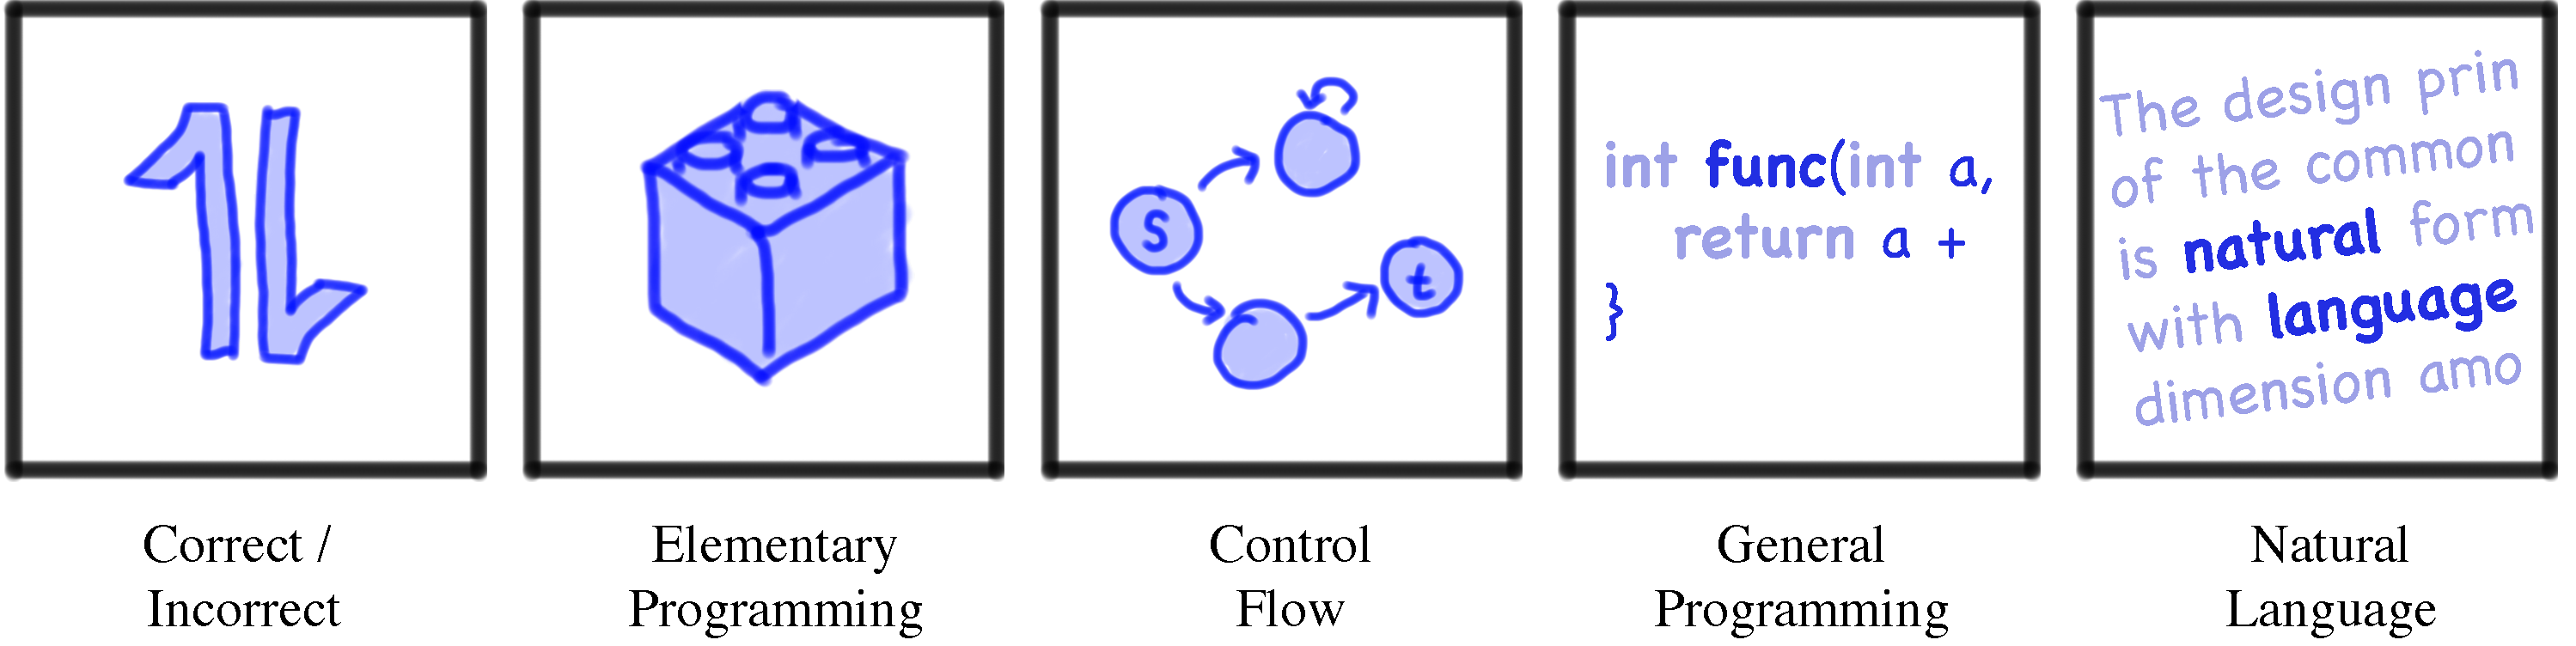
\includegraphics[width=1.0\textwidth]{img/assnType_all}
\caption[Assignment types]{
The different types of assignments covered in this thesis.
\label{fig:assnTypes}
}
\end{figure}

Specifically we identified the following different types of computer science assignments arranged in relative feedback complexity: 
\begin{enumerate}
\item Correct / Incorrect problems where students are asked either a multiple choice or short answer question and their response is coded as either being the right or wrong answer. 
\item Maze Programming assignments, which are designed for K-12 students and involve a simple maze which the students navigate using blocks that represent maze moves and may include standard control flow paradigms (like repeat, while and if)
\item Turing Complete Control Flow Programming assignments, in which students program in a language that is provably Turing complete, but does not involve user defied variables.
\item Functional Programing assignments, in which students program in a language that is turning complete and has user defined variables. We assume that programs are single threaded.
\item Natural Language assignments, in which students write up proposals and reports in English text.	
\end{enumerate}

This list is not exhaustive for all computer science assignment types. Of note, it does not include parallel programming assignments or problems from the theoretical branch of computer science. We collected at least one dataset for each of the different assignment types. See table \ref{tab:thesisDataTable} for details. 

\begin{table}[h]
 \centering
 \ra{1.3}
 \begin{tabular}{lp{1.8cm}p{1.8cm}p{1.8cm}p{1.8cm}p{1.8cm}}
   \toprule

   \tabhead{Statistic} & \tabhead{Khan \linebreak Geometry} & \tabhead{Code.org Academy} & \tabhead{Stanford CS106A} &  \tabhead{Coursera M.L.} & \tabhead{Coursera H.C.I.} \\

   \midrule

   Students & 1.0 $M$ & 1.2 $M$ & 2.7 $K$ & 26.1 $K$ & 7.2 $K$ \\
   Assignments  & 69 & 20 & 5 & 8 & 10 \\
   Submissions & 14.4 $M$ & 22.8 $M$ & 312.0 $K$ &  1.0 $M$  & 14.1 $K$ \\
   Type & Correct / Incorrect & Elementary Programs & Control Flow & Functional Programs & Natural Language \\
   Temporal & Yes & Yes & Yes & No & No \\

   \bottomrule
 \end{tabular}
 \caption[Summary of datasets]{Summary of datasets analyzed. $K = $ thousands and $M = $ millions. M.L. = Machine Learning and H.C.I = Human Computer Interaction }
 \label{tab:thesisDataTable}
\end{table}

When student work on programming assignments, we are parse their submissions into Abstract Syntax Trees (ASTs) and execute them on unit test inputs. We consider two submissions to be equal if their ASTs are identical. When possible, in addition to collecting the final submission that a student turns in for an assignment, we also collect the trajectory of partial solutions that they generate as they work their way from a blank project.

\section{Program Submission Sparsity}


An interesting observation that we made is that for every single programming assignment dataset that we analyze in this thesis, the frequency of submissions fits a Zipf's law distribution. 
\begin{figure}[ht]
\center
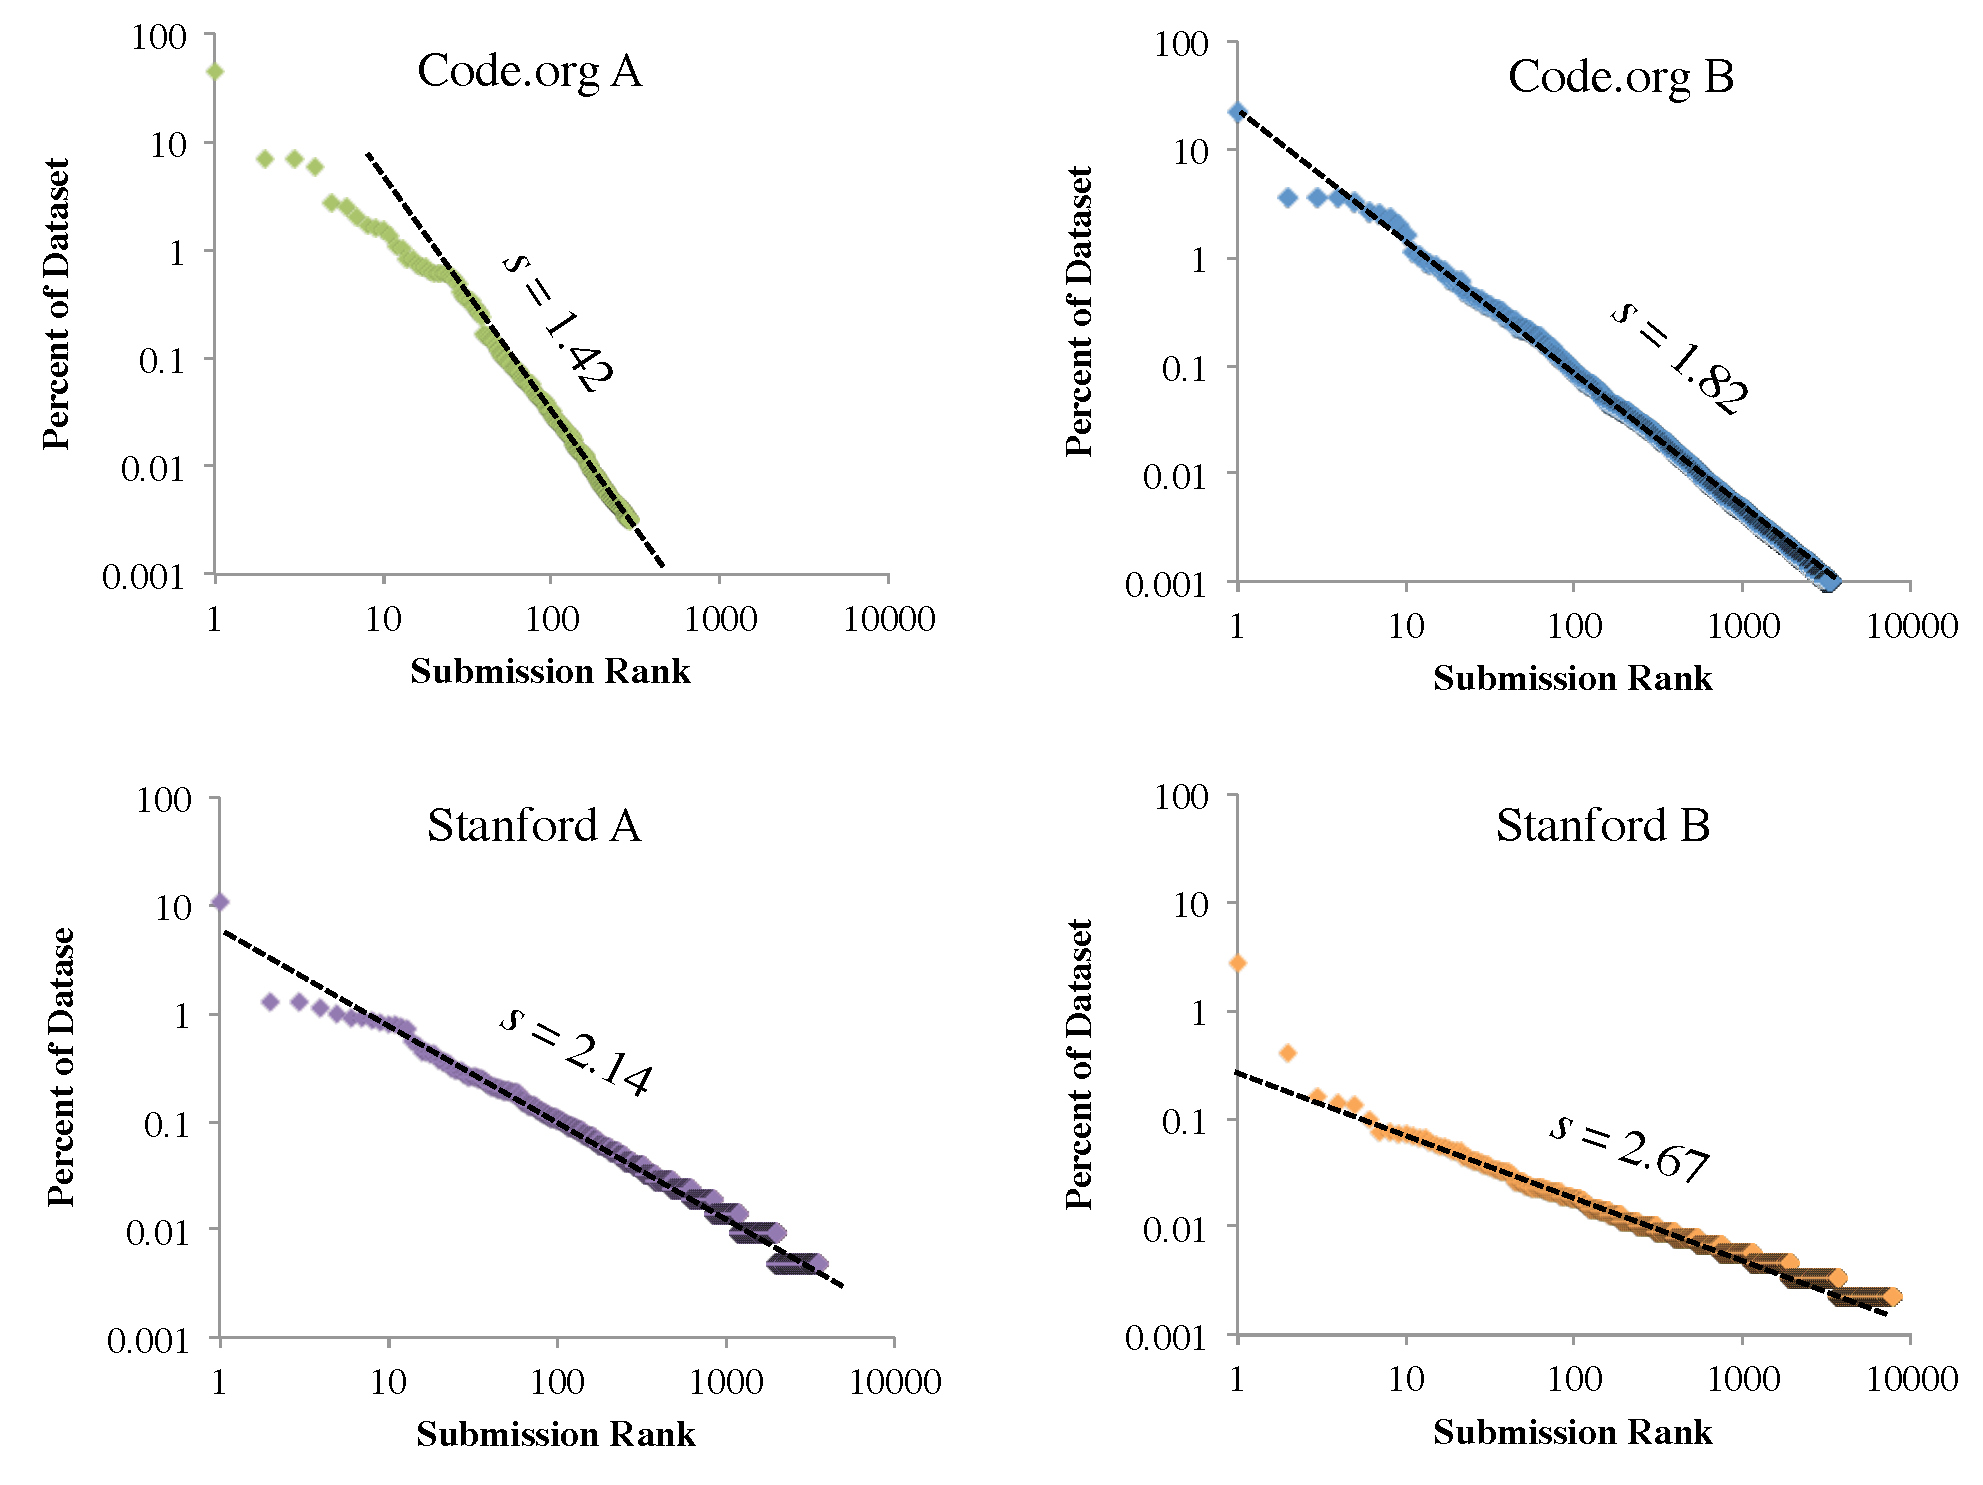
\includegraphics[width=1.0\textwidth]{img/zipfAll}
\caption[Submission Sparcity]{
Zipf plots for five assignments examined in this thesis. The designation of A and B assignments are used to differentiate different problems from the same platform. The $s$ value is the power parameter of a Zipf fit. All assignments have temporal data except for machine learning$^*$ and thus the $s$ parameter for that one assignment is not directly comparable to the others.
}
\label{fig:zipfAll}
\end{figure}
This is true for datasets where we have temporal data and datasets for which we only have final solutions. See figure \ref{fig:zipfAll}. Interestingly this trend even applies to the simplest programming assignment in the Code.org dataset where learners are only able to concatenate three commands -- and do not use any control flow elements. We have also noticed that the distribution of sub-programs also follows a Zipf's law distribution. The head of the distributions follow different patterns. The Zipf tendency seems to apply after the 10\ts{th} most common submission. Zipf law distributions often arise when data is generated in a hierarchical manner. Since students likely make a series of hierarchical decisions when solving a problem, and since programs are written in a way that produces hierarchical ASTs, it makes sense that the datasets are Zipfian. The implications are twofold. First, even for the most simple programming assignments that we look at there is a non-zero probability that a new submission will never be seen before and that will always be true regardless of how large a dataset we collect. The second implication is that we can use the exponent of the Zipf fit to compare the ``sparsity" of different programming assignments. This is particularly nice because the exponent is independent of the size of the dataset. Figure \ref{fig:zipfAll} shows the fit for all datasets for which we had temporal data. Sparsity can only be compared for datasets that were collected in a similar way (for example one cannot compare the Zipf fit for an assignment where we have all student partial solutions with one where we only have final solutions).

 An interesting observation is that the subjective ``complexity" ordering of assignment types that we chose matches the order of exponent parameters for the corresponding Zipf law distributions. This suggests one way to measure assignment complexity. Another observation is that the exponent of the Zipf distribution for the partial solutions to Stanford B is almost 3. This represents a very steep drop-off. For assignments that are more complex, the probability becomes increasingly small that one would ever observe two identical partial solutions.

\section{Approaches}

Our approach is to apply a disciplined machine learning paradigm to facilitate autonomous (or semi-autonomous) feedback at scale. Specifically we develop systems that try to capture emergent learner structures. 

\subsection{Big Picture First}

The problem of adding autonomy to the provision of feedback is hard. But the difficulty varies widely between different assignment complexities (and submission sparsity). In this dissertation we are going to start with the simplest and least sparse computer science assignments and work up in increasing levels of feedback difficulty focusing on the thematic split made in figure \cite{fig:assnTypes}. The largest difference that arises as complexity increases is that quickly program submissions become so sparse that it is hard to find temporal patterns in student work. Thus for the two simplest categories (Incorrect/Correct and Maze Programming Problems) we develop systems for autonomous feedback based on trajectories, which is a very rich source of information. However for the next two levels of complexity (Control Flow and Functional Programming) we have to first solve the problem of finding patterns in the space of submissions so that we can understand student trajectories in a more dense, latent space. One way to understand this is that we are marching down the different layers of emergent structure. The first question we ask is: can we understand students across a curriculum? Then for harder problems we ask, can we understand students as they work through a single question? For absolute hardest class of assignments, general programming tasks, we ask ourselves, can we understand how a single partial solution relates to others?

\subsection{Understand Students}

The ultimate goal of this line of research is to provide a scientific advance in our understanding of how to autonomously provide feedback to students. However there are unique challenges posed by the science of education. Three particularly notable challenges with regard to research on feedback is that (1) student experiments are expensive, (2) the mechanisms are complex so it is often hard to tease apart context or confounds and (3) learning outcomes are often multi-dimensional and long term.

It is ethical grey area to provide an experience for a student that is worse than what they would have otherwise received. There is a desire is similar to the, ``do no harm" Hippocratic oath taken in the field of medicine (where harm includes leaking any private student data). A clear example of this is that there is tremendous desire to never give feedback to students that is misleading. As a direct result experiments on live students are expensive. It is hard to convince an instructor to run a study and when a study is done it has to be performed under strict guidelines. Moreover, it is difficult to measure costs and benefits in an educational setting. Educational outcomes are multi-dimensional and involve short term and long term effects. An intervention may have broad effects on learners and testing those effects often is too invasive. Finally, even when an experiment is run on students and a reasonable education objective is selected and evaluated, it is still difficult to understand how different parts of a complicated feedback system should be attributed for observed results. As an example providing feedback often involves first autonomously understanding a student and then turning that understanding into English text that is presented to a student. It is difficult to tease the two apart.

You can think of giving feedback 
To overcome these challenges we focused on developing and testing systems that can understand students. In every chapter we identify a machine learning problem that can be used as the basis for autonomous feedback and can be directly evaluated with \emph{off-line} data. We will set out to solve these machine learning questions to the best of our ability. The task of then developing a human computer interaction system for optimally helping students is interesting and important, but outside the scope of this dissertation.

Aside: understanding can be measured either by predicting what s student will do, or by predicting what a teacher would tell a student.

\subsection{Easy to Author}

The autonomous feedback engine must be easy to author so that new activities and inspired ideas can be incorporated without much friction. Otherwise, using a machine learning system could prevent development of new assignments. There is an inherent balance between trying to maximize the quality of our feedback and to minimize teacher time. The general constraint that we held to was to keep teacher grading time the same as it would be in a traditional class of only a few dozen students.

\section{Novel Contribution}

\begin{figure}[t]
\center
   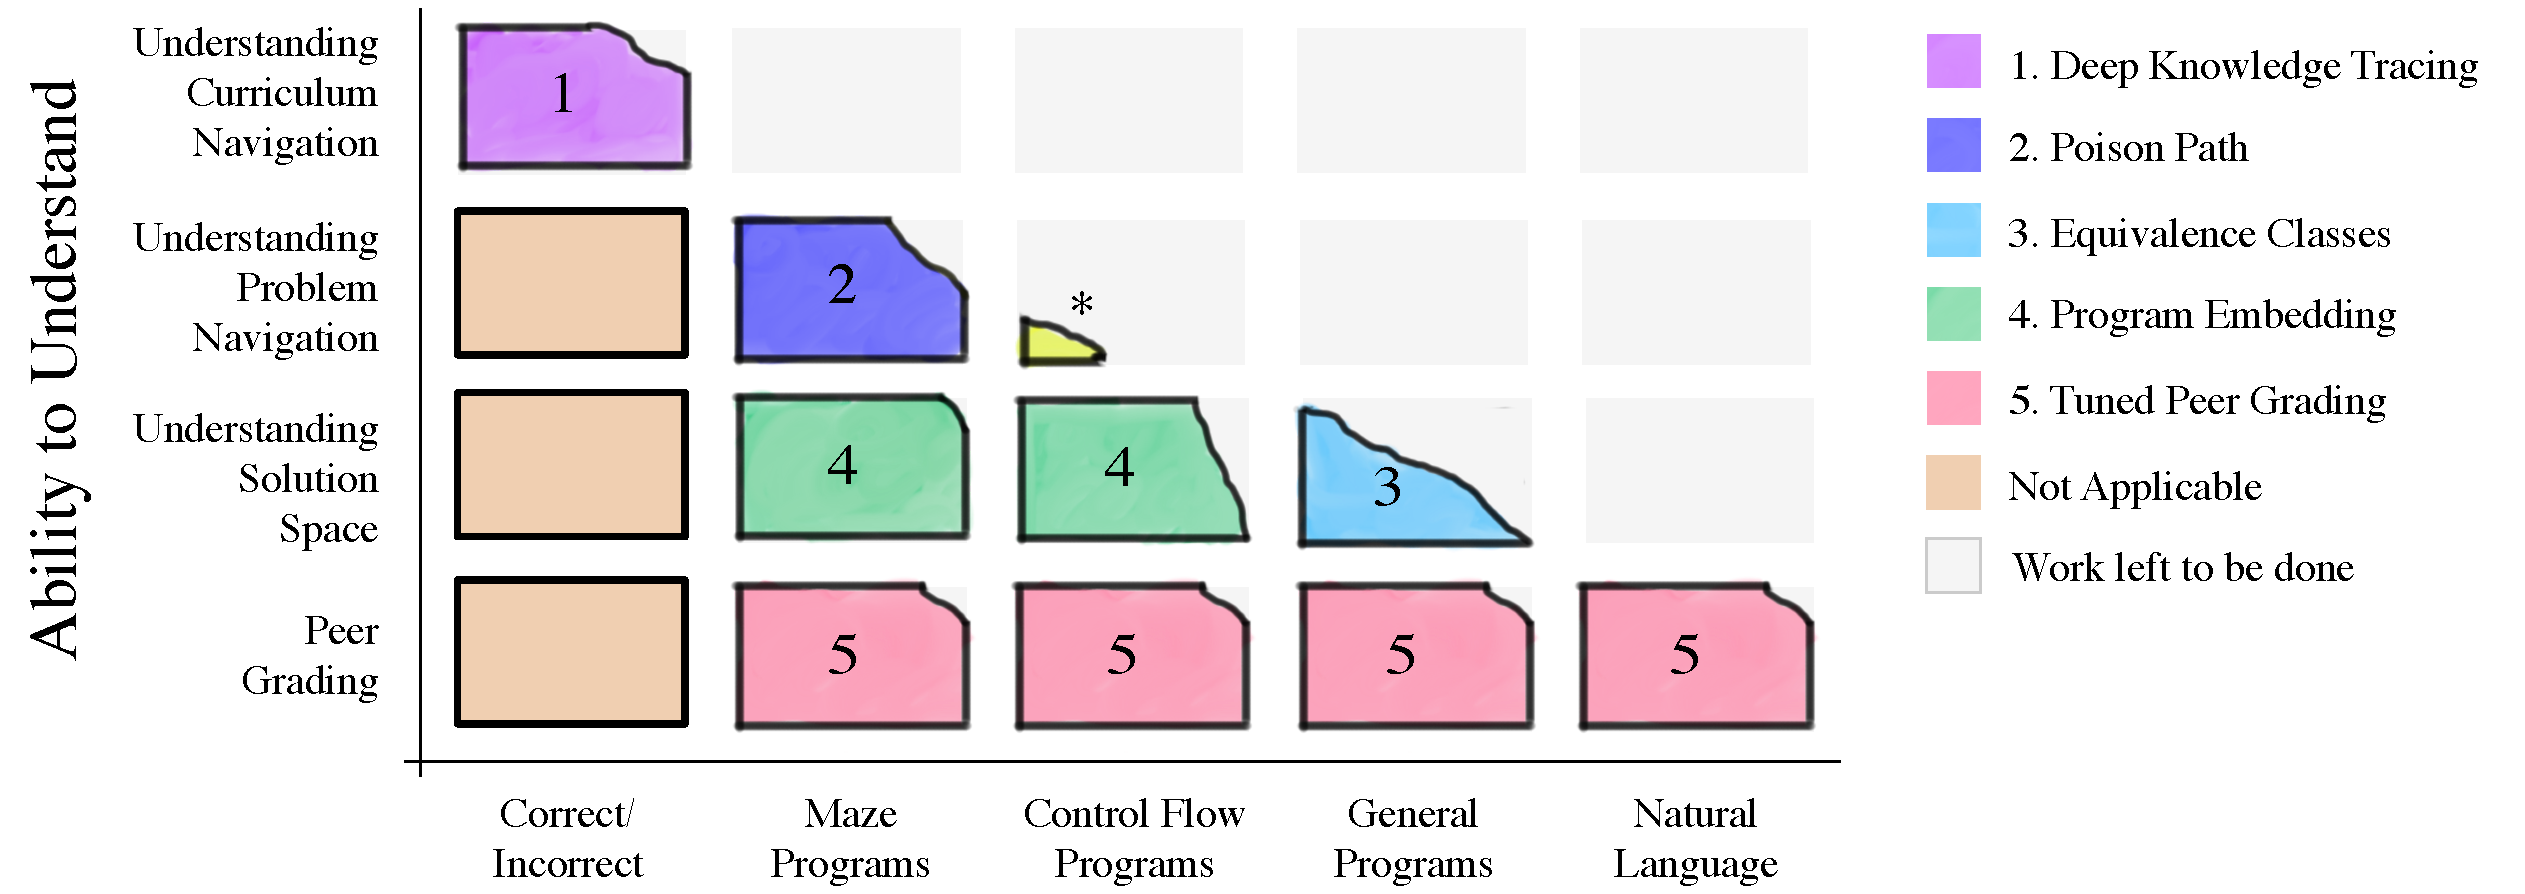
\includegraphics[width=1.0\textwidth]{img/intro-blocks.pdf}
\caption[Subjective contribution overview]{
Subjective measure of the degree to which different algorithms are able to understand students over the range of assignments that they apply.}
\label{fig:bigPicture}

\end{figure}

The challenge of how to provide autonomous feedback to students at scale remains an open problem. However I have made substantial progress towards understanding students as they learn. In each chapter we explore machine learning solutions to understanding increasingly more complex classes of assignments. 
In the first chapter we use recurrent neural networks to understand students as they solve correct/incorrect class of problems in Khan Academy. In the second chapter we find out what temporal patterns emerge when millions of students solve the same Code.org Maze assignments. In the third chapter we develop a neural network way to encode the functionality of control flow programming assignments. In the fourth chapter we present a way to autonomously discover equivalent sub-parts of general student programming assignments. Finally, in the fifth chapter we show how machine learning tools can be used to help in peer grading, the ubiquitous way to provide feedback online when autonomous methods are not available.

The most substantial contributions of this research are:
\begin{enumerate}
\item We achieved state of the art in knowledge tracing (and a 25\% increase of AUC on a standard dataset). 

\item Discovery of the Poison Path pattern in how students navigate solution spaces that both: predicts how teachers would suggest a learner make forward progress and has an almost perfect logrithmic relationship with the probability of a student succeeding in the future.

\item Two novel ways to simplify the solution space of programming assignments. A leading method to project program control flow functionality into euclidean space and an algorithm which can autonomously discover equivalent sub-parts of programs. Both means of simplifying solution expand the ability to propagate teacher feedback.

\item A novel way to `tune` the network of peer grades to simultaneously learn grading ability and assignment true scores (and a 33\% reduction in RMSE on an online design course).

\end{enumerate}
However, there are dozens of smaller corollaries that we arrived at as a result of our novel exploration of an unprecedented dataset. It is hard to quantify exactly where we stand with respect to autonomously providing feedback across the entire domain of programming assignments especially since the objectives we try to reach are slightly different for different problem types. However for each task I can subjectively express the degree to which the algorithms allow us to understand what students know. To do so I compose both (1) the degree to which a task reflects actionable understanding of a student and (2) the accuracy our algorithms were able to achieve on the task. As an example of the different utility of different prediction tasks: being able to predict exactly what a student will do represents a deeper understanding then being able to recognize that their last submissions was similar enough to another students that we can propagate feedback. For each of the new algorithms that we present I did my best to estimate algorithm ``understanding" over the range of assignments to which they are applicable. See figure \ref{fig:bigPicture}. While I have made substantial gains against the baselines of brute force annotation and propagation of feedback available from unit tests, there is still a substantial amount of room for improvement between the hull of our contemporary ability to understand students and the level that is possible.

The thesis is split into three parts. In the first part we explore how to understand students as they learn across curricula of simple answers. In the second part we will explore how to model student trajectories as they solve multi step programming tasks. In the third part we explore how to understand patterns in sparse student programs.

% include 
%One-on-one human tutoring can produce learning gains for the average student on the order of two standard deviations \cite{corbett2001cognitive}.



%\section{A Vision for the Future}
%Autonomous feedback from a system that understands learners as they navigate complex learning environments.
%In the far future, we may have powerful autonomous tutors. They will be able to understand what humans know and help them achieve learning goals in optimal ways. They will be free, or close to free. Their experience will persist. 

%The core emphasis is two solve two problems (1) Provide feedback, (2) Select appropraite material for students. 

%Achieving these milestones often involve sub-goals such as being able to predict what students will do, or how teachers would respond.

%The autonomous feedback engine must be easy to author so that new activities and inspired ideas can be incorporated without much friction.

%There are many different paths to an improved education landscape. This is just one interesting avenue.

%One reason that online is interesting is that it may enable scientific insights into learning

%Disiterata:
%Easy to author.
%Handle Richly Structured Activities


%Teachers have historically been faced with a difficult decision on how much personalized
%feedback to provide students on open-ended homework submissions
%such as mathematical proofs, computer programs or essays. On one hand, feedback
%is a cornerstone of the educational experience which enables students to
%learn from their mistakes. On the other hand, giving comments to each student
%can be an overwhelming time commitment. Hopefully autonomous feedback can be a powerful tool to help teachers of the future.

%In this work we present a set of approaches that are appropriate for different types of assignments. Ideally in the future we will be able to achieve the level of autonomous feedback we see for khan data for more complex assignments. 

%http://data.worldbank.org/indicator/SE.ENR.TERT.FM.ZS/countries/1W?display=graph

\part{How do Students Learn Across Curricula?}

\chapter{Deep Knowledge Tracing}
Based on a paper by the same name \cite{piech2015deep}\\ \emph{Proceedings of Neural Information Processing Systems (NIPS) 2015.}

\vspace{7mm}

\begin{figure}[h!]

\includegraphics[width=0.2\textwidth]{img/assnType_1}
\end{figure}

\vspace{7mm}

An especially high level of student understanding is involved in understanding how students learn across curricula. It is an important and inspiring goal of autonomous understanding of students to be able to identify that a student is not reaching their goals because they do not understand a particular foundational piece well enough. Often the signal of such a ``deal breaker" concept can be hidden in interactions with previous problems, potentially long ago in time.
In order to paint a picture of what sort of understanding we can develop about students as they learn over time, it is useful to start by understanding what is possible in a simple problem domain where it is trivial to codify student interactions with individual problems. In this chapter I explore teaching curricula from Khan Academy, and other sources, where student responses are encoded as simply ``correct" or ``incorrect". While we found it useful to start with curricula where students interacted with easily coded problems, the solutions we developed are meant to be extended to more complex domains.

Knowledge tracing---where a machine models the knowledge of a student as they interact with a series of coursework items---is a well established problem in computer supported education that has been studied for over 20 years \cite{corbett1994knowledge}. Knowledge tracing is evaluated by its ability to predict how students will perform on future questions. This ability to predict student preformance, if achieved, demonstrates a profound understanding of both a student and the material that they are working on, and as such the task has been identified as a central problem in comptuer supported education. It is the foundation beneath autonomous tutors. Improvement on this task means that resources can be suggested to students based on their individual needs, and content which is predicted to be too easy or too hard
can be skipped or delayed. Already, hand-tuned intelligent tutoring systems that attempt to tailor content show promising results \cite{polson2013foundations}. %[include ka blog post in citations]

The knowledge tracing problem is inherently difficult as human learning is grounded in the complexity of both the human brain and human knowledge.
Thus, the use of rich models seems appropriate.
However most previous work in education relies on first order Markov models with restricted functional forms. In this chapter we present a formulation that we call Deep Knowledge Tracing (DKT) in which we apply flexible recurrent neural networks that are `deep' in time to the task of knowledge tracing. 
This family of models represents latent knowledge state, along with its temporal dynamics, using large vectors of artificial `neurons', and allows the latent variable representation of student knowledge to be learned from data rather than hard-coded.
The main contributions of this work are:
\begin{enumerate}
\item A novel way to encode student interactions as input to a recurrent neural network.
\item A 25\% gain in AUC over the best previous result on a knowledge tracing benchmark. 
\item Demonstration that our knowledge tracing model does not need expert annotations.
\item Discovery of exercise influence and generation of improved exercise curricula.
\end{enumerate}

\begin{figure}[t]
\centering
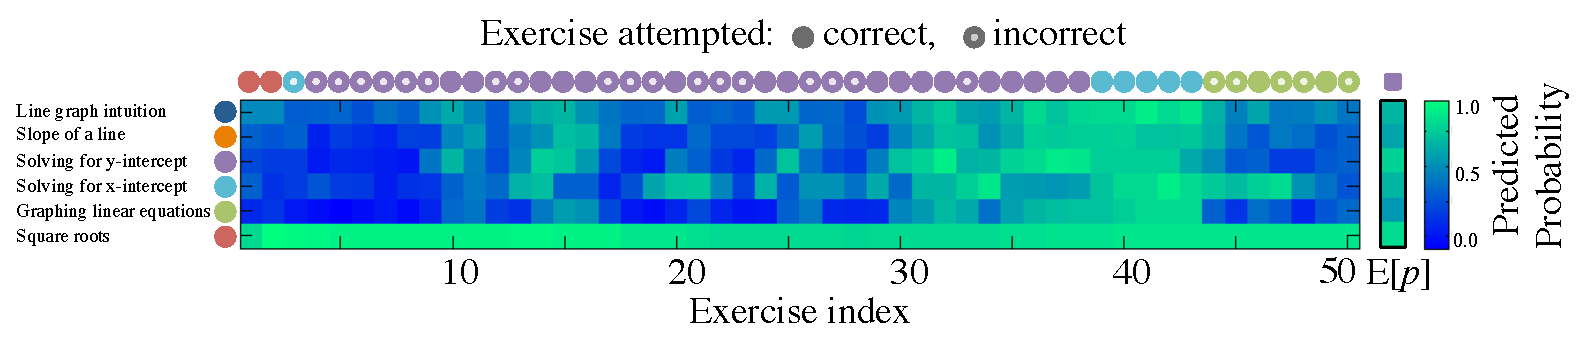
\includegraphics[width=1.0\textwidth]{img/singleStudent}

\caption[Single Khan student trace]{A single student and her predicted responses as she solves 50 exercises on Khan Academy 8th grade math curriculum. She seems to master finding x and y intercepts and then has trouble transferring knowledge to graphing linear equations.
\label{fig:singleStudent}
}

\end{figure}

\section{Knowledge Tracing}

The task of knowledge tracing can be formalized as: given observations of interactions $\mb x_0 \dots \mb x_{t}$ taken by a student on a particular learning task, predict aspects of their next interaction $\mb x_{t+1}$ \cite{corbett1994knowledge}. In the most ubiquitous instantiation of knowledge tracing, interactions take the form of a tuple of $\mb x_t = \{q_t, a_t\}$ that combines a tag for the exercise being answered $q_t$ with whether or not the exercise was answered correctly $a_t$.  When making a prediction the model is provided the tag of the exercise being answered $q_t$ and must predict whether the student will get the exercise correct $a_t$. Figure~\ref{fig:singleStudent} shows a visualization of tracing knowledge for a single student learning 8th grade math. The student first answers two square root problems correctly and then gets a single x-intercept exercise incorrect. In the subsequent 47 interactions the student solves a series of x-intercept, y-intercept and graphing exercises. Each time the student answers an exercise we can make a prediction as to whether or not she would answer an exercise of each type correctly on her next interaction. In the visualization we only show predictions over time for a relevant subset of exercise types.

In most previous work, exercise tags denote the single ``concept" that human experts assign to an exercise. These annotations are tedious to author and add friction to the introduction of new assignments.
Our model can leverage, but does not require, such expert annotation. We demonstrate that in the absence of annotations the model can autonomously learn content substructure. In the presence of annotation we can describe the relationships between the labels.

\section{Related Work}

The task of modelling and predicting how human beings learn is informed by fields as diverse as education, psychology, neuroscience and cognitive science. From a social science perspective learning has been understood to be influenced by complex macro level interactions including affect \cite{linnenbrink2004role},
motivation \cite{elliot2013handbook}
and even identity \cite{cohen2008identity}. The challenges present are further exposed on the micro level. Learning is fundamentally a reflection of human cognition which is a highly complex process. Two themes in the field of cognitive science that are particularly relevant are theories that the human mind, and its learning process, are recursive \cite{fitch2005evolution} and driven by analogy \cite{gentner1983structure}.

The problem of knowledge tracing was first posed, and has been heavily studied within the intelligent tutoring community. In the face of aforementioned challenges it has been a primary goal to build models which may not capture all cognitive processes, but are nevertheless useful.

\subsection{Bayesian Knowledge Tracing}

Bayesian Knowledge Tracing (BKT) is the most popular approach for building temporal models of student learning. BKT models a learner's latent knowledge state as a set of binary variables, each of which represents understanding or non-understanding of a single concept \cite{corbett1994knowledge}. A Hidden Markov Model (HMM) is used to update the probabilities across each of these binary variables, as a learner answers exercises of a given concept correctly or incorrectly. The formulation of the original model assumed that once a skill is learned it is never forgotten.  
Recent extensions to this model include contextualization of guessing and slipping estimates \cite{d2008more}, estimating prior knowledge for individual learners \cite{yudelson2013individualized}, and estimating problem difficulty \cite{pardos2011kt}.

With or without such extensions, Knowledge Tracing suffers from several difficulties. First, the binary representation of student understanding may be unrealistic. Second, the meaning of the hidden variables and their mappings onto exercises can be ambiguous, rarely meeting the model's expectation of a single concept per exercise.
Several techniques have been developed to create and refine concept categories and concept-exercise mappings. The current gold standard, Cognitive Task Analysis \cite{schraagen2000cognitive} is an arduous and iterative process where domain experts ask learners to talk through their thought processes while solving problems.
Finally, the binary response data used to model transitions imposes a limit on the kinds of exercises that can be modeled.

\subsection{Other Dynamic Probabilistic Models}

Partially Observable Markov Decision Processes (POMDPs) have been used to model learner behavior over time, in cases where the learner follows an open-ended path to arrive at a solution \cite{rafferty2011faster}. Although POMDPs present an extremely flexible framework, they require exploration of an exponentially large state space. Current implementations are also restricted to a discrete state space, with hard-coded meanings for latent variables. This makes them intractable or inflexible in practice, though they have the potential to overcome both of those limitations.

Simpler models from the Performance Factors Analysis (PFA) framework \cite{pavlik2009performance} and Learning Factors Analysis (LFA) framework \cite{cen2006learning} have shown predictive power comparable to BKT \cite{gong2010comparing}. 
To obtain better predictive results than with any one model alone, various ensemble methods have been used to combine BKT and PFA \cite{d2011ensembling}. Model combinations supported by AdaBoost, Random Forest, linear regression, logistic regression and a feed-forward neural network were all shown to deliver superior results to BKT and PFA on their own. But because of the learner models they rely on, these ensemble techniques grapple with the same limitations, including a requirement for accurate concept labeling.

Recent work has explored combining Item Response Theory (IRT) models with switched nonlinear Kalman filters % TODO cite jascha talk?
\cite{lan2014time}, as well as with Knowledge Tracing \cite{khajah2014integrating,khajah2014incorporating}. 
Though these approaches are promising, at present they are both more restricted in functional form and more expensive (due to inference of latent variables) than the method we present here.

\subsection{Recurrent Neural Networks}

Recurrent neural networks are a family of flexible dynamic models which connect artificial neurons over time. The propagation of information is recursive in that hidden neurons evolve based on both the input to the system and on their previous activation \cite{williams1989learning}. 
In contrast to hidden Markov models as they appear in education, which are also dynamic, RNNs have a high dimensional, continuous, representation of latent state. A notable advantage of the richer representation of RNNs is their ability to use information from an input in a prediction at a much later point in time. This is especially true for Long Short Term Memory (LSTM) networks---a popular type of RNN \cite{hochreiter1997long}.

Recurrent neural networks 
are competitive or state-of-the-art for several 
time series tasks--for instance, speech to text \cite{graves2013speech}, translation \cite{mikolov2010recurrent}, and image captioning \cite{karpathy2014deep}--where large amounts of training data are available. These results suggest that we could be much more successful at tracing student knowledge if we formulated the task as a new application of temporal neural networks.


\section{Deep Knowledge Tracing}

We believe that human learning is governed by many diverse properties -- of the material, the context, the timecourse of presentation, and the individual involved -- many of which are difficult to quantify relying only on first principles to assign attributes to exercises or structure a graphical model. Here we will apply two different types of RNNs -- a vanilla RNN model with sigmoid units and a Long Short Term Memory (LSTM) model -- to the problem of predicting student responses to exercises based upon their past activity.

\subsection{Model}

Traditional Recurrent Neural Networks (RNNs) map an input sequence of vectors $\mb x_1, \dots ,\mb x_T$, to an output sequence of vectors $\mb y_1,\dots,\mb y_T$. See Figure~\ref{fig:rnn} for a cartoon illustration. This is achieved by computing a sequence of `hidden' states $\mb h_1 , \dots , \mb h_T$  which can be viewed as successive encodings of relevant information from past observations that will be useful for future predictions. The variables are related using a simple network defined by the equations
\begin{align}
    \mb h_t &= \mathrm{tanh}\left(\mb W_{hx} \mb x_t + \mb W_{hh} \mb h_{t-1} + \mb b_h\right), \\
    \mb y_t &= \sigma\left(\mb W_{yh} \mb h_t + \mb b_y\right),
\end{align}
where both $\mathrm{tanh}$ and the sigmoid function $\sigma\left(\cdot\right)$ are applied to each dimension of the input.
The model is parameterized by an input weight matrix $\mb W_{hx}$, recurrent weight matrix $\mb W_{hh}$, initial state $\mb h_0$, and readout weight matrix $\mb W_{yh}$.
Biases for latent and readout units are given by $\mb b_h$ and $\mb b_y$.

Long Short Term Memory (LSTM) networks \cite{hochreiter1997long} are a more complex variant of RNNs that often prove more powerful.
In the variant of LSTMs we use, latent units retain their values until explicitly cleared by the action of a `forget gate'.
They thus more naturally retain information for many time steps, which is believed to make them easier to train.
Additionally, hidden units are updated using multiplicative interactions, and they can thus perform more complicated transformations for the same number of latent units.
The update equations for an LSTM are significantly more complicated than for an RNN, and can be found in Appendix \ref{app LSTM}.

\subsection{Input and Output Time Series}

In order to train an RNN or LSTM on student interactions, it is necessary to convert those interactions into a sequence of fixed length input vectors $\mb x_t$.
We do this using two methods depending on the nature of those interactions:

%\subsubsection{One-hot Encoding}

For datasets with a small number $M$ of unique exercises, we set $x_t$ to be a one-hot encoding of the student interaction tuple $h_t = \{q_t, a_t\}$ that represents the combination of which exercise was answered and if the exercise was answered correctly, so $x_t \in \mc \{0,1\}^{2M}$. We found that having separate representations for $q_t$ and $a_t$ degraded performance.

For large feature spaces, a one-hot encoding can quickly become impractically large.
For datasets with a large number of unique exercises, we therefore instead assign a random vector $\mb n_{q, a} \sim \mc N\left(0, \mb I\right)$ to each input tuple, where $\mb n_{q, a} \in \mc R^N$, and $N \ll M$. We then set each input vector $\mb x_t$ to the corresponding random vector, $\mb x_t = \mb n_{q_t, a_t}$.

%% TODO can reverse this paragraph break
This random low-dimensional representation of a one-hot high-dimensional vector is motivated by compressed sensing.
Compressed sensing states that a $k-$sparse signal in $d$ dimensions can be recovered exactly from $k \log d$ random linear projections (up to scaling and additive constants) \cite{baraniuk2007compressive}. %,candes2008introduction}.
Since a one-hot encoding is a $1-$sparse signal, the student interaction tuple can be exactly encoded by assigning it to a fixed random Gaussian input vector of length $\sim \log 2M$.
Although the current paper deals only with 1-hot vectors, this technique can be extended easily to capture aspects of more complex student interactions in a fixed length vector.% For instance, 


The output $\mb y_t$ is a vector of length equal to the number of problems, where each entry represents the predicted probability that the student would answer that particular problem correctly.
Thus the prediction of $a_{t+1}$ can then be read from the entry in $y_{t}$ corresponding to $q_{t+1}$.


\begin{figure}[t]
\begin{center}
%\framebox[4.0in]{$\;$}
%\fbox{\rule[-.5cm]{0cm}{4cm} \rule[-.5cm]{4cm}{0cm}}
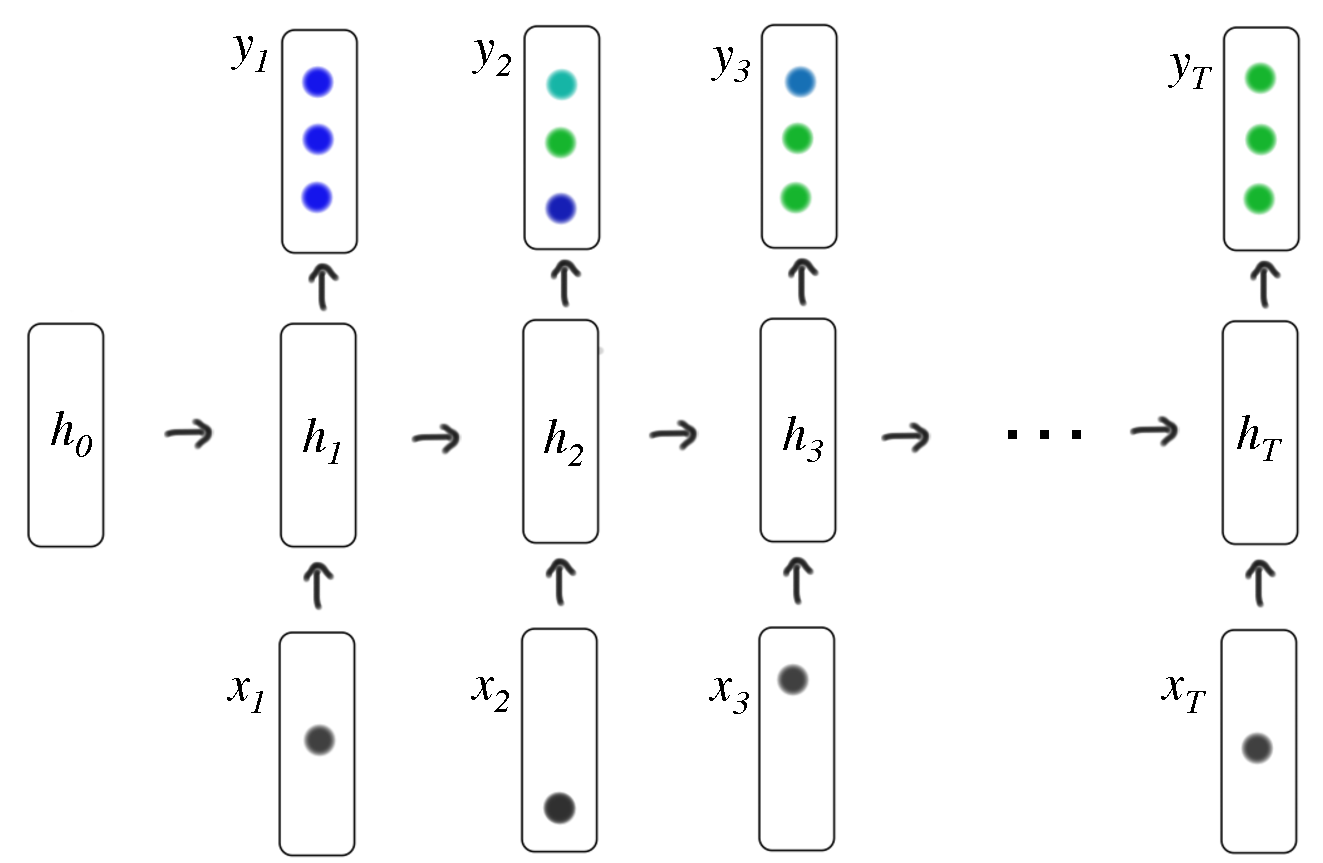
\includegraphics[width=0.7\textwidth]{img/rnn}
\end{center}
\caption[Recurrent neural network for knowledge tracing]{The connection between variables in a simple recurrent neural network. The inputs ($\mb x_t$) to the dynamic network are either one-hot encodings or compressed representations of a student action, and the prediction ($\mb y_t$) is a vector representing the probability of getting each of the dataset exercises correct.
\label{fig:rnn}
}

\end{figure}

\subsection{Optimization}

The training objective is the negative log likelihood of the observed sequence of student responses under the model. Let $\delta(q_{t+1})$ be the one-hot encoding of which exercise is answered at time $t+1$, and let $\ell$ be binary cross entropy. The loss for a given prediction is $\ell(\mb y_i^T \mb \delta\left(q_{t+1}\right), a_{t+1})$, and the loss for a single student is:
 \begin{equation}
   \begin{aligned}
         L = \sum_{t}\ell(\mb y_i^T \mb \delta\left(q_{t+1}\right), a_{t+1})
   \end{aligned}
 \end{equation}
This objective was minimized using stochastic gradient descent on minibatches.
To prevent overfitting during training, dropout was applied to $\mb h_t$ when computing the readout $\mb y_t$, but not when computing the next hidden state $\mb h_{t+1}$.
We prevent gradients from `exploding' as we backpropagate through time by truncating the length of gradients whose norm is above a threshold. For all models in this paper we consistently used hidden dimensionality of 200 and a mini-batch size of 100. 

\section{Educational Applications}

The training objective for knowledge tracing is to predict a student's future performance based on their past activity.
This is directly useful -- for instance formal testing is no longer necessary if a student's ability undergoes continuous assessment.
As explored experimentally in Section \ref{sec results},
the DKT model can also power a number of other advancements.


\subsection{Improving Curricula}

One of the biggest potential impacts of our model is in choosing the best sequence of learning items to present to a student. 
Given a student with an estimated hidden knowledge state, we can query our RNN to calculate what their expected knowledge state would be if we were to assign them a particular exercise.
% TODO we can get rid of these next sentences for space if we need to
For instance, in Figure~\ref{fig:singleStudent} after the student has answered 50 exercises we can test every possible next exercise we could show her and compute her expected knowledge state given that choice.
The predicted optimal next problem for this student is to revisit solving for the y-intercept.

We use a trained DKT to test two classic curricula rules from education literature: {\em mixing} where exercises from different topics are intermixed, and {\em blocking} where students answer series of exercises of the same type \cite{rohrer2009effects}. Since choosing the entire sequence of next exercises so as to maximize predicted accuracy can be phrased as a Markov decision problem we can also evaluate the benefits of using the $\mathrm{expectimax}$ algorithm (see Appendix) to chose an optimal sequence of problems.


\subsection{Discovering Exercise Relationships}

The DKT model can further be applied to the task of discovering latent structure or concepts in the data, a task that is typically performed by human experts.
We approached this problem by assigning an influence $J_{ij}$ to every directed pair of exercises $i$ and $j$,
\begin{align}
\label{eq influence}
J_{ij} = \frac{y\left(j|i\right)}{\sum_k y\left(j|k\right)},
\end{align}
where $y\left(j|i\right)$ is the correctness probability assigned by the RNN to exercise $j$ on the second timestep, given that a student answered exercise $i$ correctly on the first.
We show that this characterization of the dependencies captured by the RNN recovers the pre-requisites associated with exercises.




\section{Datasets}

We test the ability to predict student performance on three datasets: simulated data, Khan Academy Data, and the Assistments benchmark dataset. On each dataset we measure area under the curve (AUC). For the non-simulated data we evaluate our results using 5-fold cross validation and in all cases hyper-parameters are learned on training data. We compare the results of Deep Knowledge Tracing to standard BKT and, when possible to optimal variations of BKT. Additionally we compare our results to predictions made by simply calculating the marginal probability of a student getting a particular exercise correct.

\textbf{Simulated Data}: We simulate virtual students learning virtual concepts and test how well we can predict responses in this controlled setting. 
For each run of this experiment we generate two thousand students who answer 50 exercises drawn from $k \in {1 \dots 5}$ concepts. 
For this dataset only, all students answer the same sequence of 50 exercises. 
Each student has a latent knowledge state ``skill" for each concept, and each exercise has both a single concept and a difficulty.
The probability of a student getting a exercise with difficulty $\beta$ correct if the student had concept skill $\alpha$ is modelled using classic Item Response Theory \cite{drasgow1990item} as:
%\begin{equation}
%  \begin{aligned}
       $p(\text{correct} | \alpha, \beta) = c + \frac{1 - c}{1 + e^{\beta -\alpha}}$
%  \end{aligned}
%\end{equation}
where $c$ is the probability of a random guess (set to be 0.25). Students ``learn" over time via an increase to the concept skill which corresponded to the exercise they answered. To understand how the different models can incorporate unlabelled data, we do \emph{not} provide models with the hidden concept labels (instead the input is simply the exercise index and whether or not the exercise was answered correctly). We evaluate prediction performance on an additional two thousand simulated test students. For each number of concepts we repeat the experiment 20 times with different randomly generated data to evaluate accuracy mean and standard error.

\textbf{Khan Academy Data}: We used a sample of anonymized student usage interactions from the eighth grade Common Core curriculum on Khan Academy. The dataset included 1.4 million exercises completed by 47,495 students across 69 different exercise types. 
% NOTE -- shouldn't change this block of text -- was agreed to in email exchange with KA, and is designed to reassure that we were very careful of student privacy
It did not contain any personal information. Only the researchers working on this paper had access to this anonymized dataset, and  its use was governed by an agreement designed to protect student privacy in accordance with Khan Academy's privacy notice \cite{KAprivacy}. 
Khan Academy provides a particularly relevant source of learning data, since students often interact with the site for an extended period of time and for a variety of content, and because students are often self-directed in the topics they work on and in the trajectory they take through material.

\textbf{Benchmark Dataset}: In order to understand how our model compared to other models we evaluated models on the Assistments 2009-2010 ``skill builder" public benchmark dataset\footnote{https://sites.google.com/site/assistmentsdata/home/assistment-2009-2010-data}
. Assistments is an online tutor that simultaneously teaches and assesses students in grade school mathematics. It is, to the best of our knowledge, the largest publicly available knowledge tracing dataset \cite{feng2009addressing}. 

\section{Results}\label{sec results}

\begin{table*}\centering
\ra{1.3}
\begin{tabular}{@{}llllcllll@{}}
\toprule
& \multicolumn{3}{c}{$Overview$} & \phantom{abc} &
 \multicolumn{4}{c}{$AUC$} \\
\cmidrule{2-4} 
\cmidrule{6-9}  
Dataset & Students & Exercise Tags & Answers && Marginal & BKT & BKT* & DKT \\ 
\midrule
Simulated-5 & 4,000 & 50 & 200 K && 0.64 & 0.54 & - & 0.75 \\
Khan Math  & 47,495 & 69 & 1,435 K && 0.63 & 0.68 & - & 0.85 \\
% Bridge to Algebra & 3,310 & 1,829 & 8,918,000 && ? & ? & ? \\
Assistments & 15,931 & 124 & 526 K && 0.62 & 0.67 & 0.69 & 0.86 \\
\bottomrule
\end{tabular}
\caption[Knowledge tracing accuracy]{AUC results for all datasets tested. BKT is the standard BKT. BKT* is the best reported result from the literature for Assistments. DKT is the result of using LSTM Deep Knowledge Tracing.
% Note that the best performing models in Bridge to Algebra make use of student performance {\em after} as well as before the test set, while DKT restricts itself to a causal prediction of student performance.
\label{table:results}
}

\end{table*}

On all three datasets Deep Knowledge Tracing substantially outperformed previous methods. On the Khan dataset using a LSTM neural network model led to an AUC of 0.85 which was a notable improvement over the performance of a standard BKT (AUC = 0.68), especially when compared to the small improvement BKT provided over the marginal baseline (AUC = 0.63). See Table~\ref{table:results} and Figure~\ref{fig:khanRoc}. On the Assistments dataset the DKT had a 25\% gain on the previous best reported result (AUC = 0.86 and 0.69 respectively) \cite{pardos2011kt}. The gain we report in AUC compared to the marginal baseline (0.24) is more than triple the gain achieved on the dataset to date (0.07).

The prediction results from the synthetic dataset provide an interesting demonstration of the capacities of deep knowledge tracing. Both the LSTM and RNN models did \emph{as well} at predicting student responses as an oracle which had perfect knowledge of all model parameters (and only had to fit the latent student knowledge variables). See Figure~\ref{fig:toyAcc}. In order to get accuracy on par with an oracle the models would have to mimic a function that incorporates: latent concepts, the difficulty of each exercise, the prior distributions of student knowledge and the affine transformation of learning that happened after each exercise. In contrast, the BKT prediction degraded substantially as the number of hidden concepts increased as it doesn't have a mechanism to learn unlabelled concepts.


 \begin{figure*}[ht]
 \centering
 \subfigure[]
 {
 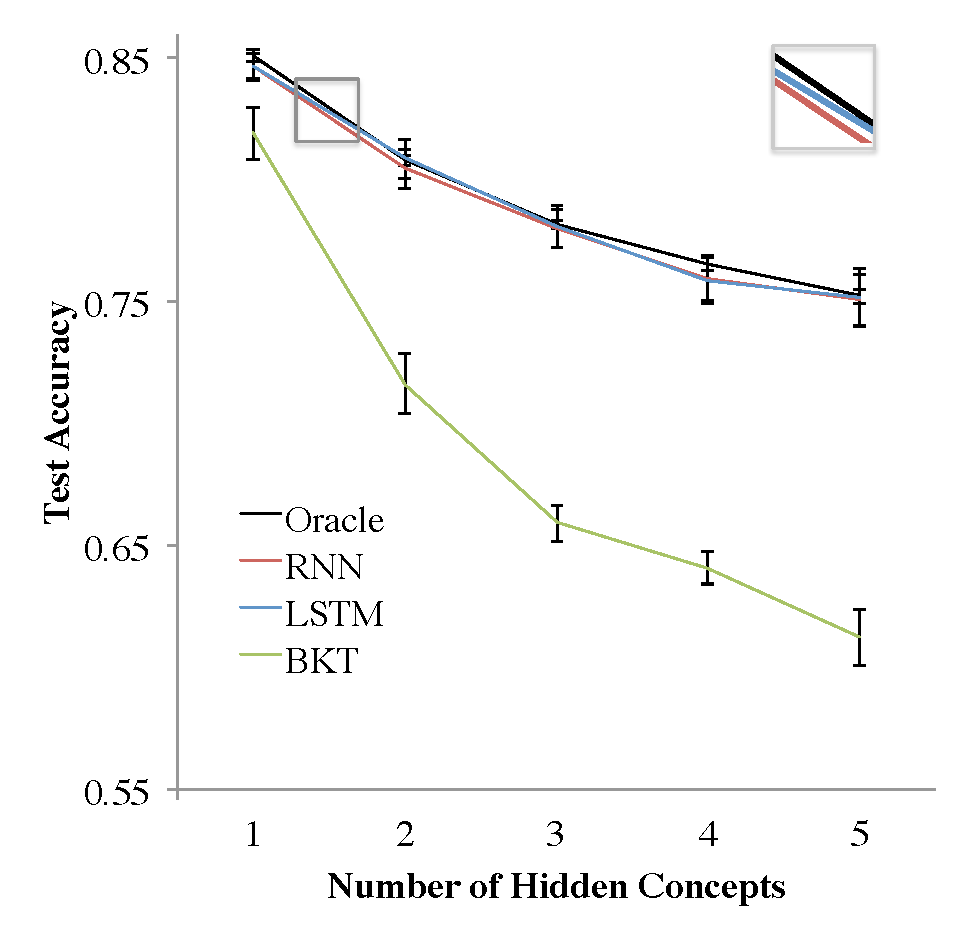
\includegraphics[width=0.45\textwidth]{img/toyAcc}
 \label{fig:toyAcc}
 }
 \subfigure[]
 {
 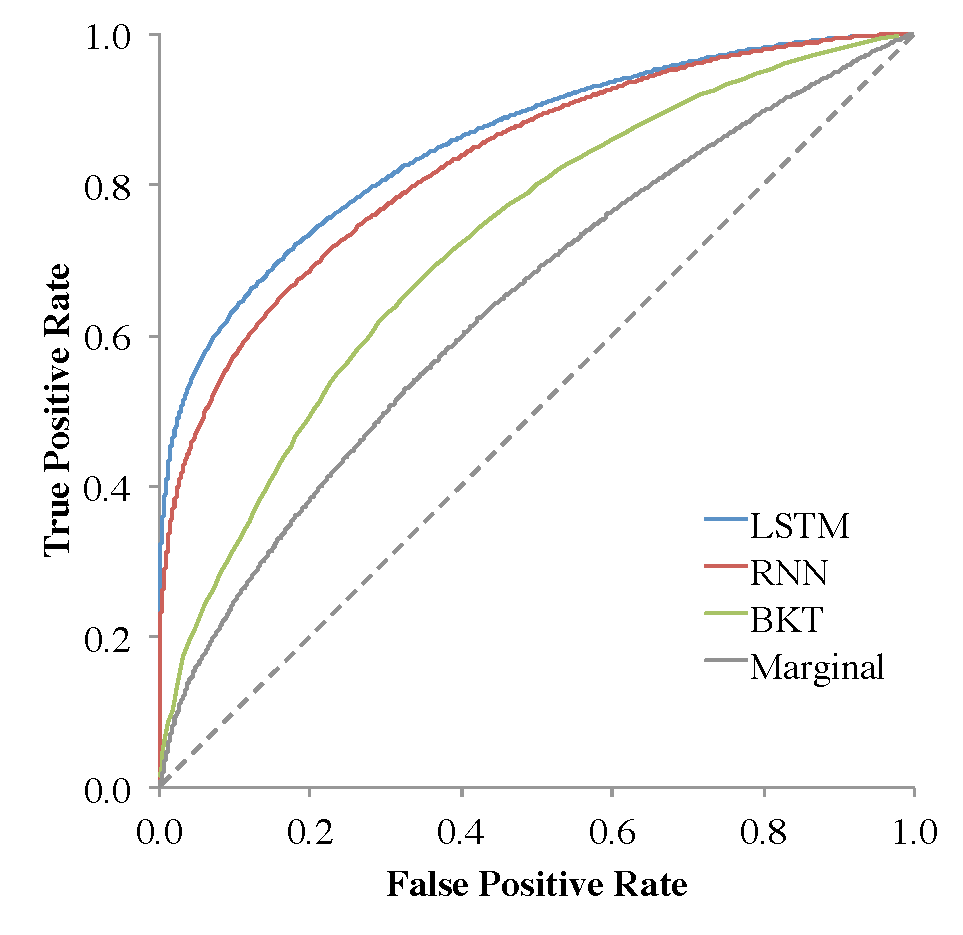
\includegraphics[width=0.45\textwidth]{img/khanRoc}
 \label{fig:khanRoc}
 }
 
 \caption[Deep Knowledge Tracing accuracies]{Prediction results for (a) simulated data and (b) Khan Academy data.}

 \end{figure*}

 \subsection{Optimal Curriculum}
We tested our ability to intelligently chose exercises on a subset of five concepts from the Assistment dataset. For each curricula method, we used our DKT model to simulate how a student would answer questions and evaluate how much a student knew after 30 exercises. We repeated student simulations 500 times and measured the average predicted probability of a student getting future questions correct. In the Assistment context the blocking strategy had a notable advantage over mixing. See Figure~\ref{fig:curriculum}. 

\begin{figure}[h]
 \centering
 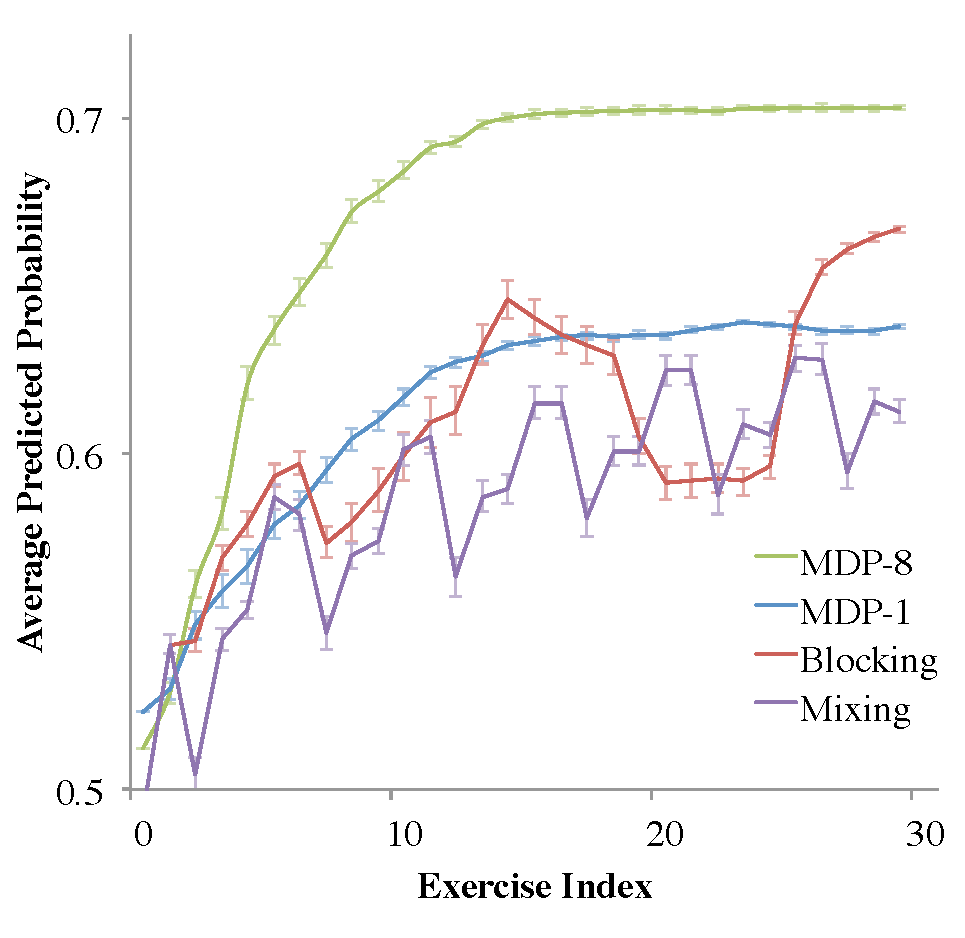
\includegraphics[width=0.45\textwidth]{img/curriculum}
 \caption[Curriculum evaluation]{Predicted knowledge on Assistments data for different exercise curricula. Error bars are standard error of the mean.}
 \label{fig:curriculum}
\end{figure}

While blocking performs on par with solving $\mathrm{expectimax}$ one exercise deep (MDP-1), if we look further into the future when choosing the next problem we come up with curricula where students have higher predicted knowledge after solving fewer problems (MDP-8). 


\subsection{Discovered Exercise Relationships}\label{sec ex rel}



The prediction accuracy on the synthetic dataset suggest that it may be possible to use DKT models to extract the latent structure between the assessments in the dataset. The graph of our model's conditional influences for the synthetic dataset reveals a perfect clustering of the five latent concepts (see Figure~\ref{fig:conceptClusters}),
with directed edges set using the influence function in Equation \ref{eq influence}.
An interesting observation is that some of the exercises from the same concept occurred far apart in time. For example, in the synthetic dataset, where node numbers depict sequence, the 5th exercise in the synthetic dataset was from hidden concept 1 and even though it wasn't until the 22nd problem that another problem from the same concept was asked, we were able to learn a strong conditional dependency between the two.

\begin{figure}[!h]
\centering
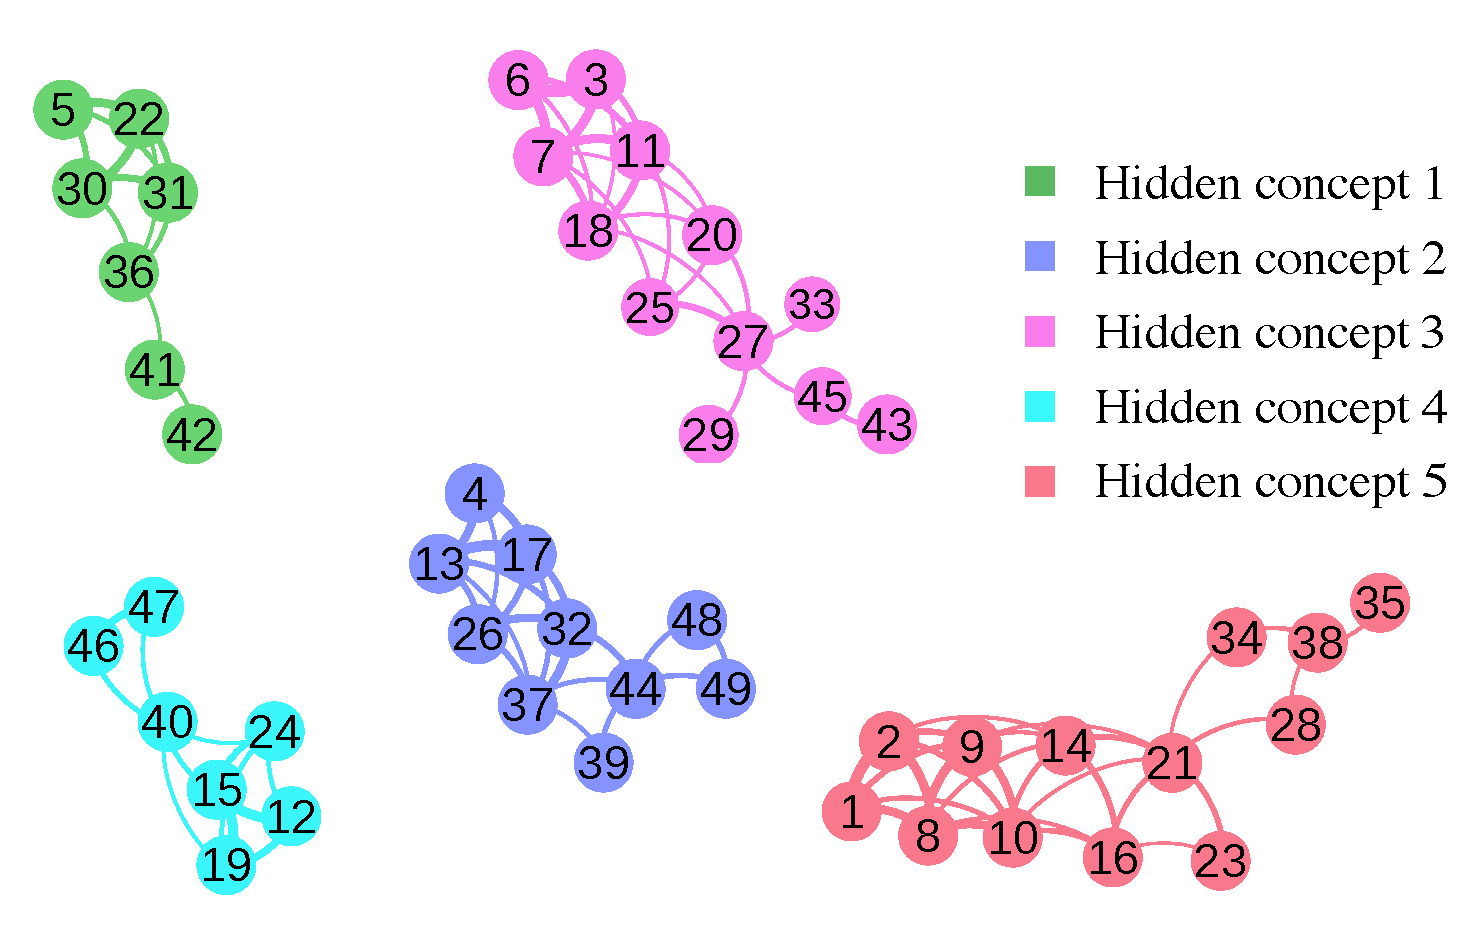
\includegraphics[width=0.6\textwidth]{img/conceptClusters_synth}
\caption[Conditional influences synthetic data]{Graphs of conditional influence between exercises in the synthetic dataset according to the DKT. We observe a perfect clustering of latent concepts in the synthetic data. 
\label{fig:conceptClusters}
}
\end{figure}

We analyzed the Khan dataset using the same technique. The resulting graph is a compelling articulation of how the concepts in the 8th grade Common Core are related to each other (see Figure~\ref{fig:conceptClusters}. Node numbers depict exercise tags).
We restricted the analysis to ordered pairs of exercises $\{A,B\}$ such that after $A$ appeared, $B$ appeared more than 1\% of the time in the remainder of the sequence).
To determine if the resulting conditional relationships are a product of obvious underlying trends in the data we compared our results to two baseline measures (1) the transition probabilities of students answering $B$ given they had just answered $A$ and (2) the probability in the dataset (without using a DKT model) of answering $B$ correct given a student had answered $A$ correct.
Both baseline methods generated discordant graphs, which are shown in the Appendix. While many of the relationships we uncovered may be unsurprising to an education expert, they were derived autonomously from data, and the subtleties may be useful for course design. Above all the results are an affirmation that the DKT network learned a coherent model.


\begin{figure}[!h]
\centering
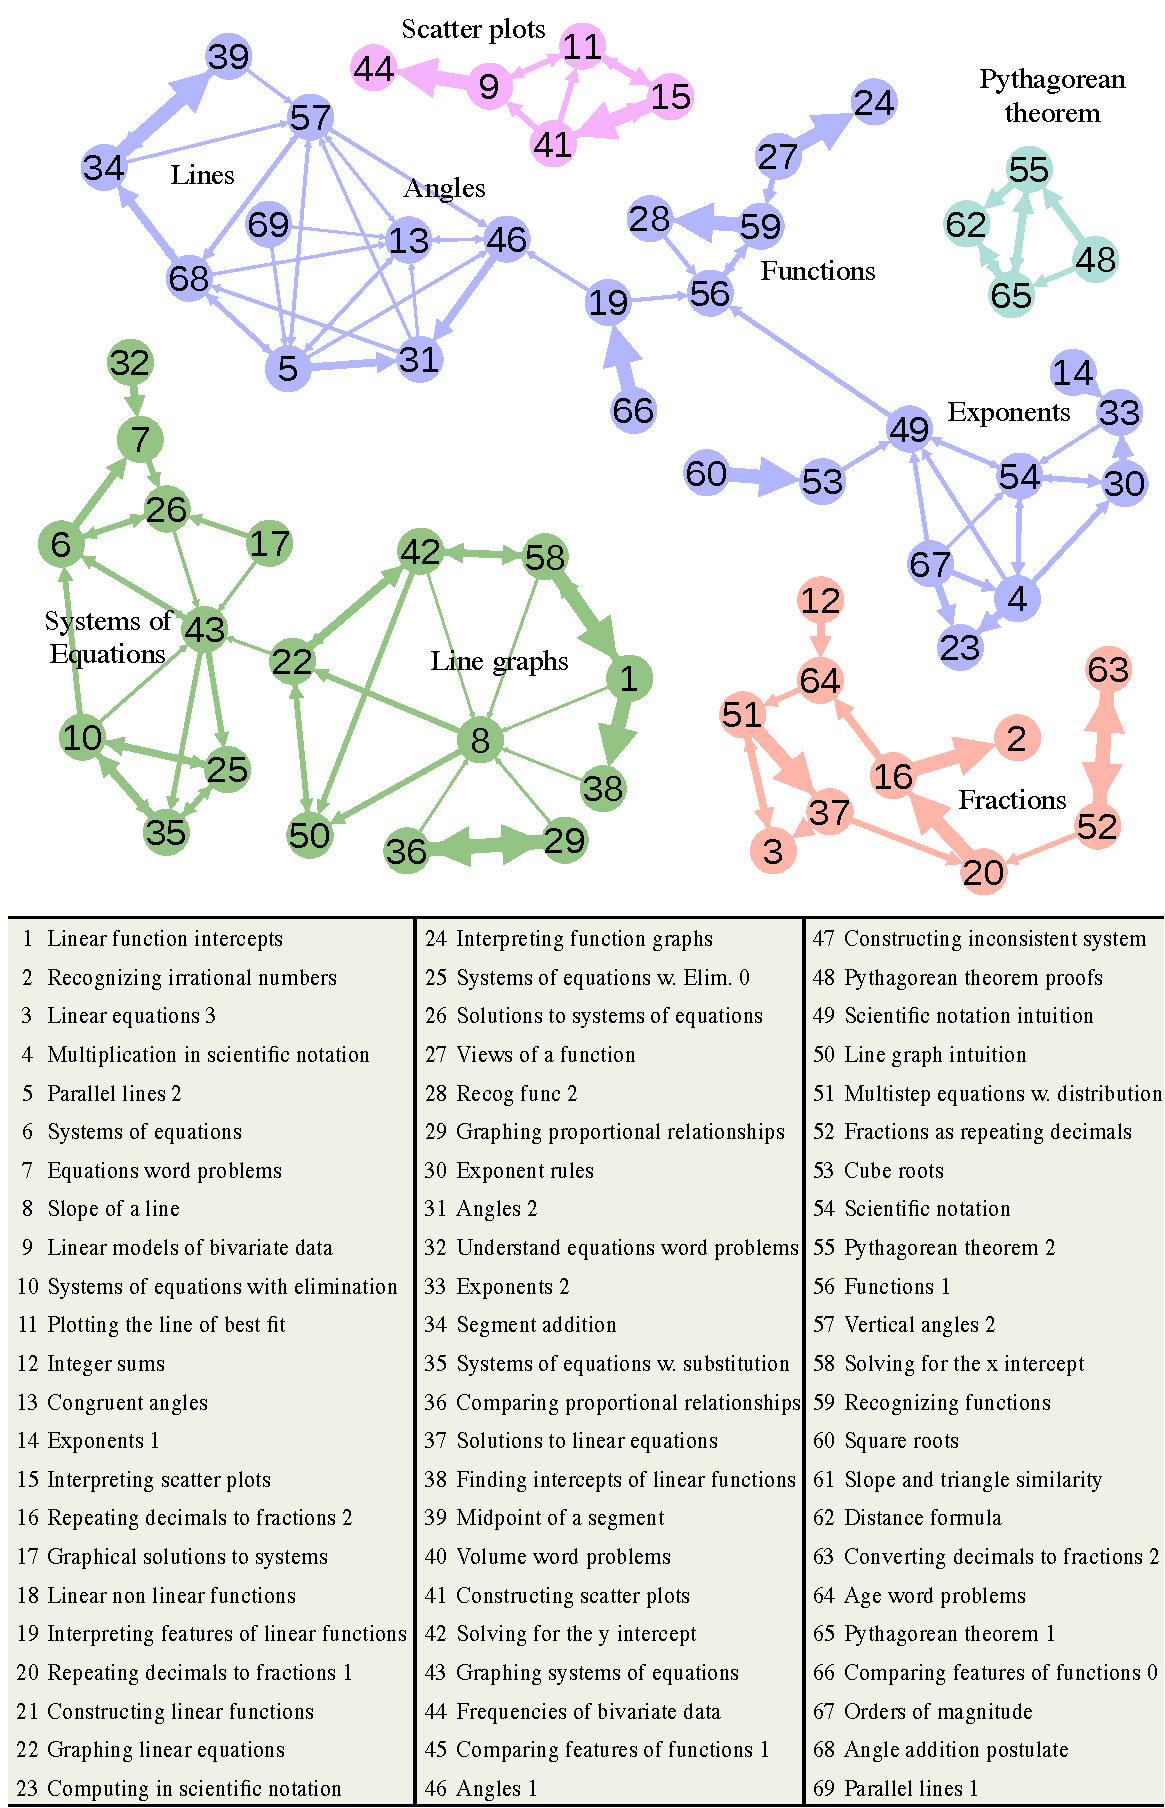
\includegraphics[width=0.7\textwidth]{img/conceptClusters_khan}
\caption[Conditional influences Khan]{A convincing depiction of how 8th grade math Common Core exercises influence one another.
Arrow size indicates connection strength. Note that nodes may be connected in both directions. Edges with a magnitude smaller than 0.1 have been thresholded. 
\label{fig:conceptClusters}
}

\end{figure}


\section{Discussion}

In this paper we apply RNNs to the problem of knowledge tracing in education, showing improvement over prior state-of-the-art performance on the Assistments benchmark and Khan dataset.
Two particularly interesting novel properties of our new model are that (1) it does not need expert annotations (it can learn concept patterns on its own) and (2) it can operate on any student input that can be vectorized. One disadvantage of RNNs over simple hidden Markov methods is that they require large amounts of training data, and so are well suited to an online education environment, but not a small classroom environment. 

The application of RNNs to knowledge tracing provides many directions for future research. Further investigations could incorporate other features as inputs (such as time taken), explore other educational impacts (such as hint generation, dropout prediction), and validate hypotheses posed in education literature (such as spaced repetition, modeling how students forget).
Because DKTs take vector input it would be theoretically possible for us to track knowledge over more complex learning activities.

In an ongoing collaboration with Khan Academy, we plan to test the efficacy of DKT for curriculum planning in a controlled experiment, by using it to propose exercises on the site. 

A foundational piece to our ablity to understand students learning over the span of a curriculum is that we were working with assignments where it was trivial to encode the students work (they either answered a question correctly or incorrectly). The future of education will incoporate more nuanced questions than multiple choice or short answer. Thus an especially interesting extension is to trace student knowledge as they solve open-ended programming tasks, and importantly incorporating these sorts of interactions is possible in Deep Knowledge Tracing in a way that was not possible with Bayesian methods since the take vector input
. The next crucial question to ask is: how can we understand student learning trajectories as they work on rich assignments?


\part{How do Students Explore Problem Space?}

\chapter{Problem Solving Policies}
Based on a paper: Autonomously Generating Hints by Inferring Problem
Solving Policies \cite{piech2015autonomously} \\ \emph{Learning at Scale 2015.}

\vspace{7mm}

\begin{figure}[h!]
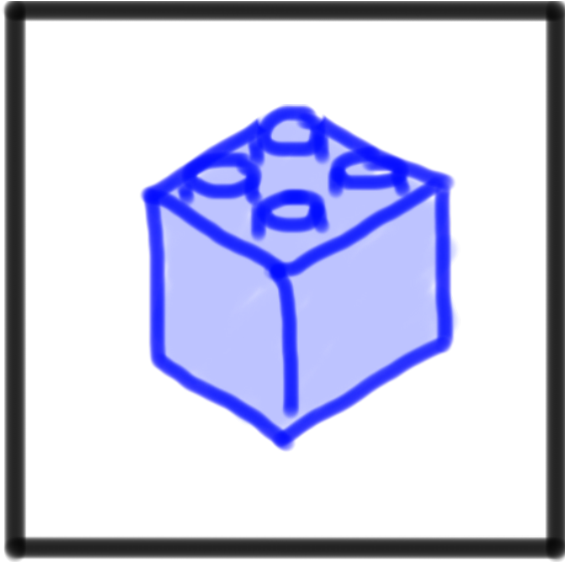
\includegraphics[width=0.2\textwidth]{img/assnType_2}
\end{figure}

\vspace{7mm}

When students solve challenges that involve layered steps of problem solving -- for example when they solve programming assignments -- the trajectory that they take to navigate to their final answer contains rich information about what they know. In order to take this next, deeper step into understanding how student learn we chose to study students working on Maze Programming Assignments. These assignments which are designed for K-12 students and use blocks that represent standard control flow paradigms (like repeat, while and if) are ideal because the number of unique programs that students generate is quite small, and thus easier to understand.

%Deep Knowledge tracing is a powerful tool for the domain of assignments where student responses can be encoded as ``correct" or ``incorrect". For more complex domains where students produce rich, structured responses it is no longer sufficient to simply track their work on the granularity of one binary input per assignment. When a student solves a richly structured assignment they produce a series of partial solutions and need assistment intermediately.
%In this domain we focus on predicting what a teacher would do.
%One of the reasons that I believe recurrent neural networks are hard to apply to the task of tracing knowledge as a student works on a multi stage assignment is that predicting what a student will do next is particularly difficult given the sparsity of the solution space.

Exploring the whole sequence of steps a student takes to produce work, and the patterns that emerge from thousands of such sequences is fertile ground for a richer understanding of learning. In this chapter we uncover a pattern in student learning that can both predict the way an expert teacher would encourage a student to make forward progress and predict a student's future retention. We discovered this pattern by observing historical data of students learning in the Code.org `Hour of Code,' curriculum (which is to the best of our knowledge the largest online course to date). We approached this problem by first focussing on trying to find patterns that allow us to predict how teachers would suggest students make forward progress. Not only are such predictions a signal that we understand students, additionally they can form the basis for an effective hint generation system. The algorithms that we develop are more accurate than current state-of-the-art methods at recreating expert suggestions, are easy to implement and scale well. We then show that the same framework which motivated the hint generating algorithms suggests a sequence-based statistic that can be measured for each learner. We discover that this statistic is highly predictive of a student's future success. 

A motivating case study is the set of assessments in the Code.org Hour of Code course. Code.org is a non-profit organization that led a coordinated effort to have every K-12 student in the United States complete an hour worth of computer science. As part of the initiative Code.org hosted an Hour of Code curriculum: a series of twenty introductory programming ``challenges" with instructional videos. In the year and a half since they launched, over 27 million learners have tried their curriculum and it has been taught in over 90 thousand classrooms making it, to the best of our knowledge, the largest MOOC to date. In the challenges students generate programs by putting together blocks of code. The open ended nature of coding, and the many avenues that students can take to get to the solution both make the challenges appealing learning activities, and prevent Code.org from being able to provide expert feedback to stuck students. 

The main contributions of this chapter are:
(1) a family of algorithms which can accurately predict how experts believe learners should make forward progress from a partial solution, based on historical data (2) a related per-student statistic generated from how a student solves a challenge that correlates strongly with future performance and (3) a unified comparison of previously published algorithms. These results speak to a deeper theme: \emph{how} students solve assignments is an under utilized, important lens into what students know and what feedback future students will need.

\section{Problem Solving Policy}

The Hour of Code challenges take several steps for a student to solve. At each point in time, the student's current work constitutes a partial solution $\psi \in S$ where $S$ is the set of all possible responses. As the student works on the assessment they will transition through a series $T = \{\psi_0, \psi_1, ... , \psi_n$\} of partial solutions from step $0$, when they have done no work, to step $n$ when they have either reached the solution or given up. 
We propose that generating feedback autonomously for an assessment of this nature can be seen as the composition of two tasks: 
\begin{enumerate}
\item Deciding for any learner what partial solution an educational expert would suggest they transition to next. 
\item Choosing how to communicate that information to the student such that they improve on a learning objective. 
\end{enumerate}
The first task can be interpreted as ``learning to understand students" and the second can be interpreted as ``using that knowledge to aid students." We suggest that both of the decoupled tasks can be solved and tested independently. The objective of this paper is to solve the former problem by learning what we call a Problem Solving Policy (PSP): a decision for any partial solution as to what next partial solution a student should take (see definition \ref{pspDef} and the example in figure \ref{fig:policy}). Using historical data we generate PSPs for challenges in the Hour of Code and evaluate to what extent they capture expert opinion.

\begin{defo}
Problem Solving Policy (PSP). \\ 
Let $S$ be the set of partial solutions.
A problem solving policy $\pi : S \rightarrow S$ specifies a partial-solution $s' = \pi(s)$ for all $s \in S$.
\label{pspDef}
\end{defo}

\begin{figure}
\centering
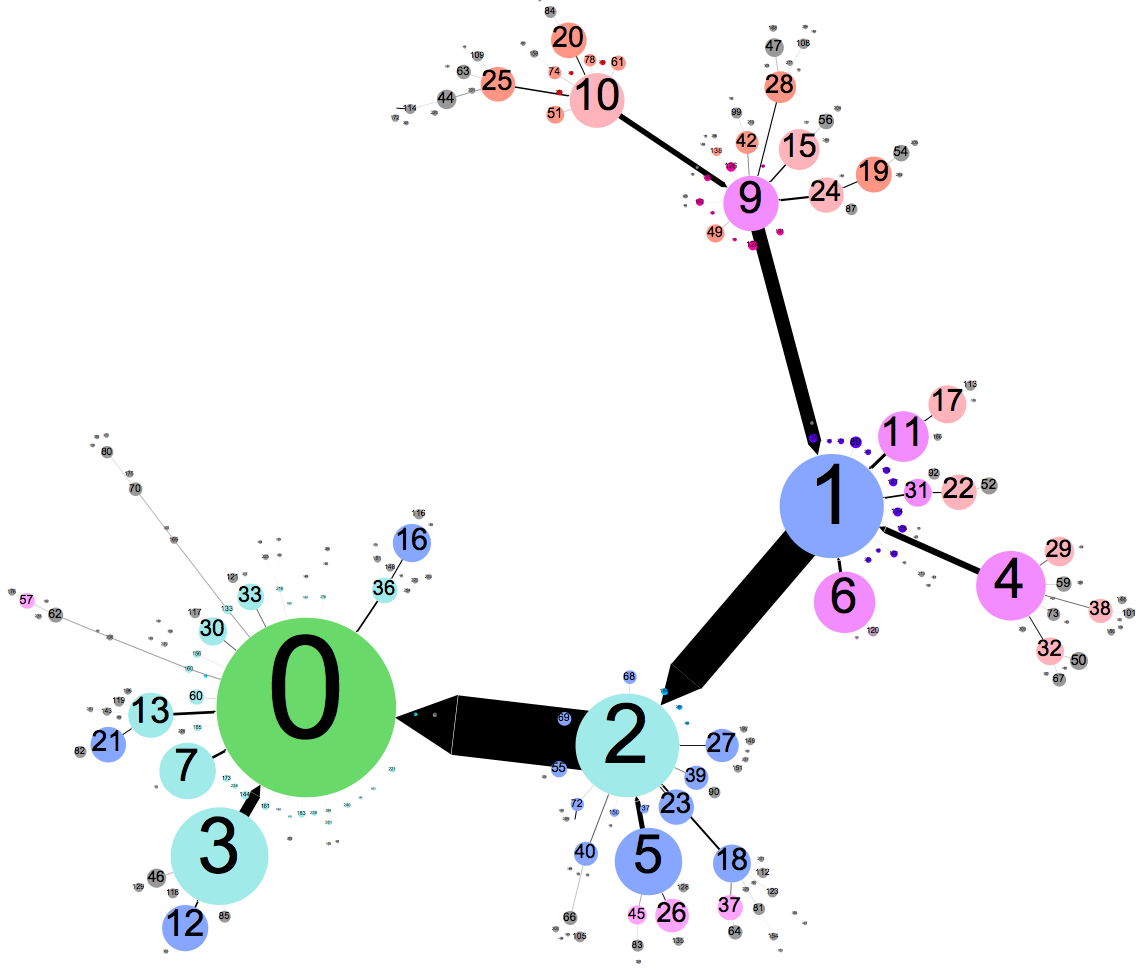
\includegraphics[width=1.0\columnwidth]{img/policy3}
\caption[Example problem solving policy]{A visualization of a problem solving policy generated for an early Hour of Code challenge. Each node is a unique partial solution, node 0 is the correct answer. The edges show what next partial solution we think an expert would suggest students move towards.}
\label{fig:policy}
\end{figure}

Note that the definition for a PSP makes the Markov assumption as no partial solution other than a student's current state is considered in the policy mapping. 

A PSP provides a foundation for generating formative feedback. For a given partial solution, there are many types of issues a student could have: they may have missed a step, made a mistake, have compounded mistakes, or possibly they are on the right path and simply need to keep going. An ideal PSP captures these diverse needs. It selects the single part of the partial solution the student should work on first and denotes how they should do so. Importantly, the PSP can also be evaluated independently from the actual feedback given to students (e.g. via a hint generation) given a ground truth dataset composed of expert evaluations on how they would push a student forward. 

Our hypothesis is that for large classes like Code.org there are patterns which materialize in how the many previous students have navigated from an empty project to the final answer which can be leveraged to learn how students should move forward from any $\psi \in S$. For example, if ten thousand students had at some point all submitted the exact same partial solution with the same set of mistakes, it seems reasonable that the best way forward is illuminated by the way that crowd then went on to fix their programs. Surprisingly, we found that many of the most obvious statistics that could be calculated from historical data or static analysis were not particularly useful. 

\section{Related Work}

Giving automated hints for richly-structured assessments at scale is a task with a long history of research that includes fields as diverse as intelligent tutors, theorem provers, crowd sourcing and peer grading.

This work expands upon research towards data-driven PSPs by the Intelligent Tutor (IT) community. In particular a similar problem was posed in Rivers' and Koedinger's paper Automating Hint Generation with Solution Space Path Construction \cite{rivers2014automating}. Rivers et al presented an algorithm which introduces the heuristic that popular partial solutions tend to correspond to good next steps. The Hint Factory by Barnes et al uses a historically trained Markov Decision Problem (MDP) formulation \cite{barnes2008toward}. While both papers present algorithms, the PSPs they generate were not directly measured for quality and the algorithms have previously not been compared to one another. There has been research from the field of static analysis which present alternative ways to generate PSPs. Singh et al suggest ways to find shortest path edits to a solution for programming problems, work which builds off a community of static analysis and theorem prover research \cite{singh2013automated}  \cite{cheang2003automated}. One contribution of this paper is to recreate the IT algorithms and a static analysis algorithm so that we can evaluate them all on the same dataset. 

There are a range of ways to generate feedback for richly-structured assessments at scale that do not involve first learning a PSP. One particularly interesting approach is to crowd source feedback for students \cite{weld2012personalized}, an idea which can be extended to the programming domain \cite{watson2012bluefix}. While it would take a substantial amount of work to give feedback to all answers in rich assessments Nguyen et al suggests ways to identify functionally equivalent programs which can share annotations \cite{nguyen2014codewebs} \cite{rivers2012canonicalizing}. An appealing idea is to have students reflect on what mistakes they made after solving a problem, but this idea does not apply to our setting where students are as young as five years old. At what point is a student ready to consciously reflect on the challenges that they faced? Peer grading is one of the most common solutions for giving feedback to complex assignments at scale in massive open online courses \cite{kulkarni2013peer}; however, it can only be used to give feedback on a final submissions, not hints to a stuck student. Moreover asking students to peer grade programs would have a dramatic impact on the experience of the Hour of Code if used for each challenge.

Cognitive tutors are a compelling approach towards hint generation  \cite{ritter2007cognitive} \cite{aleven2002effective}. They are well rooted in educational theory and have been shown to be pedagogically successful. However, the effort required to author a cognitive model, a necessary component, increases with the number of unique answers a student can produce. For richly-structured assignments such as the one in Code.org this approach does not scale well. Similarly there is a literature of scientists trying to understand, via observation, how student's solve programming challenges. The frameworks developed have engendered better teaching techniques but not at-scale autonomous hints \cite{fitzgerald2008debugging} \cite{ahmadzadeh2005analysis}.

The problem of generating a PSP can be seen as an instance of more general problems. There is a clear parallel between generating a PSP and autonomous decision making \cite{puterman2009markov}. Finding a PSP could be expressed as a route planning task \cite{szczerba2000robust} and historical data could be viewed as item responses where students vote on ways to make forward progress \cite{whitehill2009whose}.  

One of the aims of this work is to enable further comparative research. To this end we will share relevant code and annonomized, aggregate data:
\url{http://stanford.edu/~cpiech/codedotorg.html}

\section{Data from Code.org}





In the Hour of Code website, students write programs to solve maze world puzzles. Each time a learner runs their program, a symbolic representation of their current work is recorded. When the learner submits a final answer, or stops working on a challenge, the learner’s partial solutions are composed into a raw series. There is a simple mechanism to test if two symbolic representations are identical.

\begin{figure}[h]
	\centering
	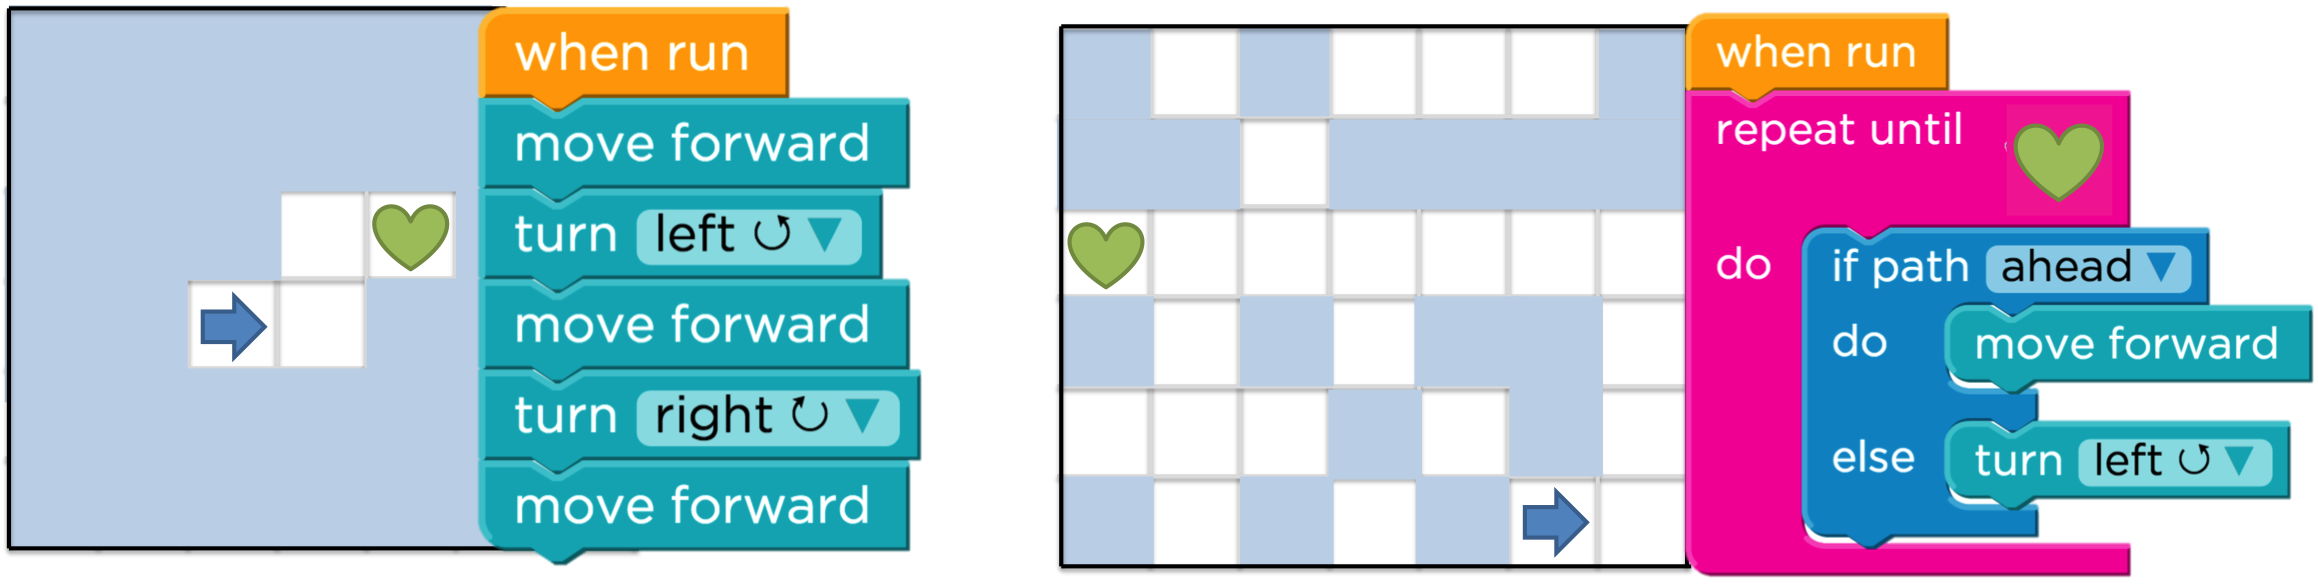
\includegraphics[width=0.8\columnwidth]{img/problems3.png}

	\caption[Schematic of Code.org problems]{Schematic of the maze and example solution for \Pa (left) and \Pb (right). The arrow is the agent and the heart is the goal.}
	\label{fig:hocExample}
\end{figure}

The dataset for this paper is the series of partial solutions from all logged in students from December 2013 to March 2014. In that time Code.org gathered over 137 million partial solutions. Retention was quite high relative to other contemporary open access courses, see figure \ref{fig:retention}. Volunteered information from 19.5\% of the logged in users gives us a window into the demographic makeup of the learners: 59\% are male and 41\% are female. The average age is $\mu$ = 13.2, $\sigma$ = 4.3 years old with the age range spanning from 5 to 98 years old.


In this analysis we focus on two problems \Pa and \Pb which are representative of different levels of complexity. See figure \ref{fig:hocExample} for a schematic of the problems, and the solution code. The solution to \Pa, which was the fourth challenge in the twenty challenge curriculum, requires students to string together a series of moves and turns. The solution to \Pb, which was the eighteenth challenge, requires an if/else condition inside a for loop: the most advanced concept in the hour of code. 

Surprisingly, while the challenges only required a few lines of code, the number of unique partial solutions submitted by the logged in users was in the tens of thousands (See table \ref{tab:dataTable}). We define unique submissions to be ones with unique abstract syntax trees. For \Pb, even if we only look at programs with ten lines of fewer, there are around 10 million hypothetical unique partial solutions. It is partially for this reason that it is so difficult to crowd source hints. However, the occurrence of partial solutions is not evenly distributed and notable impact could be had by annotating the most popular partial solutions. Figure \ref{fig:coverage} shows the percent of submissions that would be covered by generating hints for the most popular partial submissions. In order to cover 90\% of submissions for \Pb one would need to annotate 7,127 unique programs. Code.org crowd sources hints but to this date has only solicited tens of annotations per challenge.

In the raw series of data, a student could make incremental changes between runs or make large changes between runs. To normalize out this difference we interpolated each student's series so that transitions between partial solutions constituted exactly one program edit (as allowed by the website interface). To interpolate we first made a ``legal move graph" of all the ways that users can move between partial solutions using single edits. The legal move graphs for \Pa and \Pb have average out-degrees of 8.5 and 4.3 respectively. Then for every sequence of states $(a, b)$ in the raw series that is not in the legal move graph, we replaced the sequence with the most likely path that a student would have taken along the legal move graph to get from $a$ to $b$. Transition probabilities were calculated through the observed transitions along the legal move graph with a baysian prior. We made a Markovian assumption that the probability of each transition was independent of previous transitions taken. Interpolation results in a new series $T = \{\psi_0, \psi_1, ... , \psi_n\}$. We define a student to have been ``successful" if $\psi_n$ was the challenge solution. 

\begin{table}[t]
  \centering
  \ra{1.3}
  \begin{tabular}{lll}
    \toprule
    
    \tabhead{Statistic} & \tabhead{\Pa} & \tabhead{\Pb}  \\
    \midrule
    Students Studied & 509,405 & 263,569 \\
    Submissions & 1,138,506 & 1,263,360 \\
    Unique Submissions & 10,293 & 79,553 \\
    Pass Rate & 97.8\% & 81.0\%\\
    \bottomrule
  \end{tabular}
  \caption[Problem solving policy dataset summary]{Summary of the dataset analyzed.}
  \label{tab:dataTable}
\end{table}

To evaluate policies, we gathered expert gold standard data for both challenges. A group of seven computer science educators each labeled hundreds of student programs (225 for \Pa  and 268 for \Pb\hspace{-0.5mm}) with the partial solution they suggest a student who ran that program should transition to next. Inter rater reliability showed a notable degree of agreement. The Fleiss Kappa score \cite{fleiss1981measurement} was 0.58. All conflicting codings were discussed and multiple correct ways forward were allowed when there was disagreement.

\begin{figure*}
\centering
\subfigure[]
{
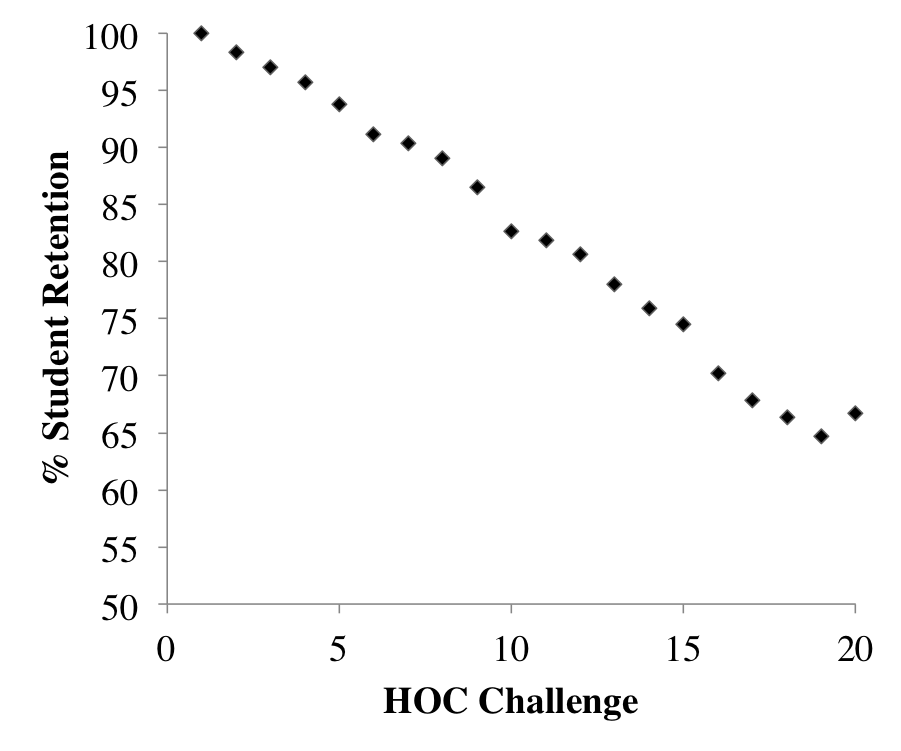
\includegraphics[width=.48\textwidth]{img/retention.png}
\label{fig:retention}
}
\subfigure[]
{
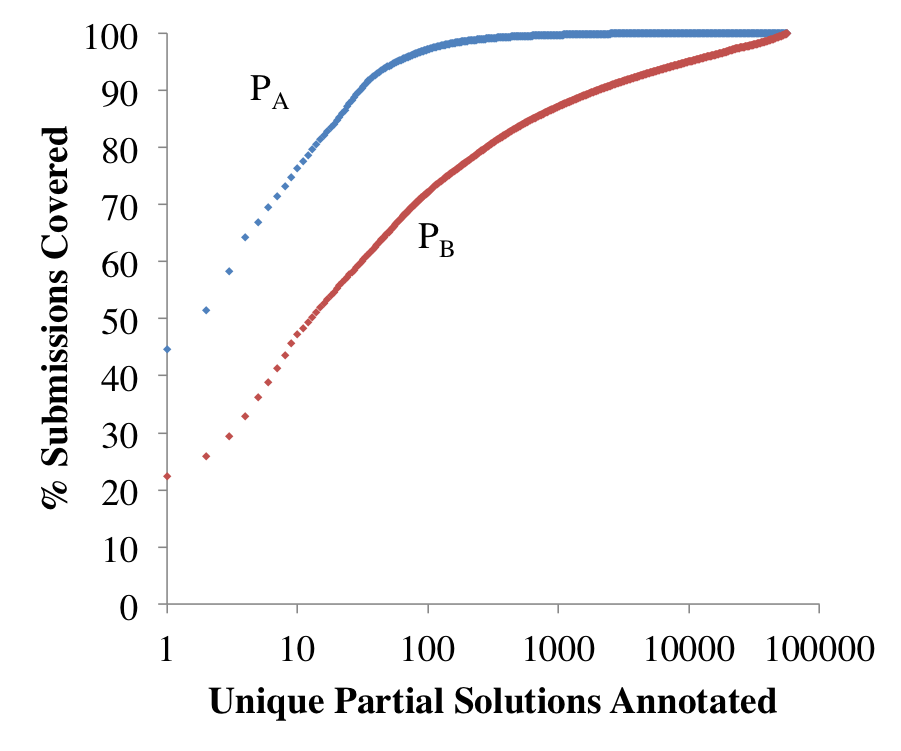
\includegraphics[width=.48\textwidth]{img/annotationImpact.png}
\label{fig:coverage}
}

\caption[Overview of Code.org data]{
\subref{fig:retention} Percent of students who finished the first problem in the hour of code that solve the remaining ones.
 \subref{fig:coverage} The percent of submissions that are covered by annotating the most popular partial solutions. 
 }
\label{tab:predacc}
\end{figure*}

\section{Methods}

The main objective of our research is to find the best algorithm for generating a PSP. We tested three classes of solutions: Desirable Path algorithms, previously proposed algorithms and vanilla baseline algorithms. The general intuition is that though individuals navigate partial solutions in misleading ways, wisdom emerges from the cohort of students.

\subsection{Desirable Path Algorithms}

Historical data of students shows many interesting patterns.
But turning that data into a prediction of how experts would suggest a learner make forward progress is a complicated task. Students are learning. Many students are working through systematic misunderstandings and this process is reflected in their navigation through partial solutions. 



Moreover, partial solutions that are further off the most common path-to-solution, are visited by students that are less likely to act like experts. See figure \ref{fig:confidence}. This is an especially salient confound as these are precisely the partial solutions where feedback to a student would be most necessary. One way to think about this problem is that uncommon partial solutions usually reflect mistakes on the part of a student. Knowing that a student has made a mistake, one can suppose that they are less likely than the average student to make future transitions which agree with expert suggestions. For example: in \Pa    a common incorrect partial solutions is a program that makes the agent move twice (and thus crash into the wall) before turning left. The population of students who have submitted a program that crashes into a wall already have misconceptions as to the dynamics of the challenge. Though the expert recommended way to make forward progress is to remove one of the move statements, by far the most common next transition that those students make is to change their turn left to a turn right, which takes them even further from the solution.


\begin{figure}
\centering
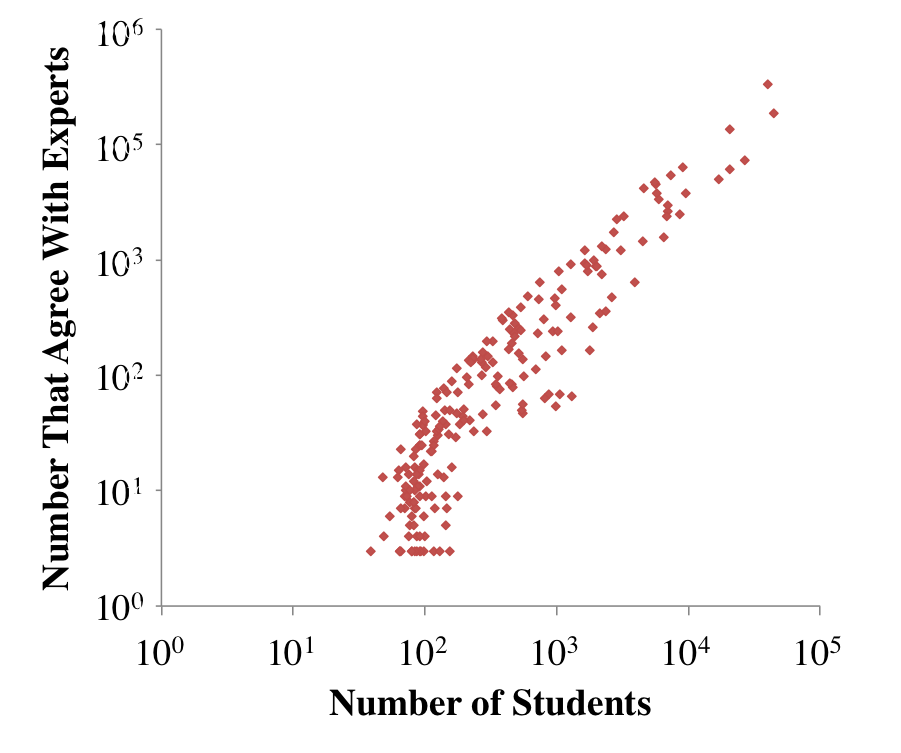
\includegraphics[width=0.5\columnwidth]{img/wrongVsPopularity.png}
\caption[Partial solution popularity vs probability of optimal progress]{How does node popularity relate to number of students who agree with experts?}
\label{fig:confidence}
\end{figure}


If we base our policy off of the transitions of students, we will often be trusting a group of learners that we know have already made a mistake. This biased sample limits our ability to understand the path-to-solution that \emph{would} have been the most popular \emph{if} partial solutions were all visited by ideal students. This raises a question: how can we know anything about a given partial solution that isn't collected solely from the students that submit said partial solution? 

One answer to that question is that we know the relative popularity of a partial solution based on how often it was submitted. Unlike transition counts, which sample from a biased population, the number of times a partial solution is seen in our dataset, ``partial solution counts," reflect a property of that partial solution for the average student in the dataset. A relatively high popularity suggests that the average student in the sample found the partial solution to be a useful way-point on a path-to-solution. A relatively low popularity suggests that the average student did not. By creating algorithms based off of this statistic we can avoid the confound that arises from the uneven distribution of ability across partial solutions.

Even if we make the assumption that partial solution counts reflect a global desirability of that partial solution how can we turn that intuition into a PSP? The solution is not as easy as: for any partial solution, chose the legal move such that the next partial solution has a high count. That strategy, more often than not, would encourage the student to delete any progress they have made. The most popular partial solution is the empty program and partial solutions which are further from the empty program tend to be less popular. Instead, to generate a PSP we must seek a balance between visiting desirable partial solution and making forward progress. We believe that teachers strike this balance by considering the entire path that they would expect a student to go down. Algorithmically this can be interpreted as searching for an optimally desirable path-to-solution. Once a path-to-solution is decided upon, the PSP function is simply the first step in that path.

We propose a desirable path theory which assumes that (a) desirability of a partial solution to the average student is a function of historical counts and (b) experts suggest that learners make progress along the most desirable path-to-solution. We present two algorithms that derive from this theory. 

\subsubsection{Poisson Path}

The first algorithm that we propose based on the desirable path theory is the Poisson Path.

We define the Poisson Path from a partial solution $s$ to be the path from $s$ to a perfect solution with the smallest expected time to be generated by the average successful student. We assume that the amount of time required for an average student to generate a partial solution is a Poisson process whose rate parameter can be estimated via the partial solution count from the student's population. This assumption is founded in the belief that the prototypical student prefers partial solutions that are easy to generate.

Given these assumptions the Poisson Path $\gamma(s)$ is:
\begin{align*}
\gamma(s)=\argmin_{p \in Z(s)}{\sum_{x \in p}{\frac{1}{\lambda_x}}}
\end{align*}
Where $Z(s)$ are all the paths-to-solution from $s$ and $\lambda_x$ is the number of times partial solution $x$ is seen in successful student data. To generate a PSP we set $\pi(s)$ to be the first partial solution in the path $\gamma(s)$. 



\vbox{
\begin{defo}
Poisson Path. \\ 
Let $G$ be a graph traversed by agents. Assume for a node $x \in G$, the time required for an agent to visit that node varies as an $exponential(\lambda_x)$ where $\lambda_x$ is a Poisson rate parameter. 

The expected time until an agent visits a given node $x$ is $\frac{1}{\lambda_x}$ and the expected time until an agent generates each node in a path $p$ is 
$\sum_{x \in p}{\frac{1}{\lambda_x}}$


The Poisson Path is the path from a node $s$ to a terminal with the smallest expected time required to be generated by an agent. Of all the paths $Z(s)$ from $s$ to the terminal, the path with the smallest expected time is 
\begin{align*}
\gamma(s)=\argmin_{p \in Z(s)}{\sum_{x \in p}{\frac{1}{\lambda_x}}}
\end{align*}
\label{pcpDef}
\end{defo}
}

Computing the Poisson Path can be solved using a simple reduction to Dijkstra's shortest path algorithm. We construct a graph where for all legal transitions $a \rightarrow b$ we add an edge with cost $\frac{1}{\lambda_b}$. A Dijkstra search for the shortest path to any solution over this graph will return the Poisson Path. Dijkstra's algorithm is easy to implement and runs in $O(n\log n)$ time for a graph with $n$ partial solutions. To prevent repeat submissions from having an undue influence on our partial solution counts we remove all cycles from student series before we count occurrences.


\subsubsection{Independent Probable Path}
A second algorithm that we propose based on the desirable path theory, is the Independent Probable Path. 

This algorithm tries to find the path-to-solution from a given partial solution that would have been the most probable for an average successful student who we would hypothetically start at that partial solution. For the average student we do not know partial solution transition probabilities. We instead know that the probability of the average student submitting a partial solution is proportional to the partial solution count. Using these submission probabilities we can calculate the markov-zero most likely path-to-solution for a randomly sampled student in the class. The Independent Probable Path $\gamma(s)$, is calculated as:
\begin{align*}
\gamma(s)&=\argmax_{p \in Z(s)}{\prod_{x \in p}{p(\psi_t = x)}} \\
         &=\argmax_{p \in Z(s)}{\sum_{x \in p}{\log(\frac{\lambda_x}{k})}}\\
         &=\argmin_{p \in Z(s)}{\sum_{x \in p}{-\log(\frac{\lambda_x}{k})}}
\end{align*} 


Where $Z(s)$ are all paths in the legal move graph from $s$ to the solution, $\lambda_x$ is the count of successful students who submitted $x$ and $k$ is the total number of submissions. This algorithm can also be reduced to an instance of Dijkstra's shortest path. 

\subsection{Baseline Algorithms}
Several algorithms for generating PSPs have been proposed in recent publications. Here we provide a brief overview of the algorithms and any modifications that were made to better fit the algorithms to the Code.org context. We also explore a series of simpler, direct measures. 

\subsubsection{Markov Decision Problem}
As proposed by Barnes and Stamper we can generate a PSP by formulating student transitions as a Markov Decision Problem (MDP) and learning an optimal policy. An MDP is defined by specifying states, actions, rewards over states and transition probabilities. In the Barnes et al formulation the states are the set of partial solutions, actions are the legal changes to a program allowed in the interface and the reward of a partial solution is set to be 100 if it is a correct answer, 0 otherwise. Of note, the transition probability between partial solutions $a$ and $b$ is defined as $p(\psi_{t+1} = b | \psi_t = a)$.

In a standard MDP the transition probability is the chance of ending up in a state given one's previous state \emph{and} an action the policy decided to perform. Applied to this setting we would need to know the probability of a student going from one partial solution to another \emph{if} we were to suggest a particular next state. In the historical data available to Barnes et al and in the Code.org context that conditional probability is unknown; we can't observe how our suggestions would effect student transitions. Instead, as in Barnes et al, we assume that a student's transition probability is independent of the partial solution we chose for them. The MDP has a single hyper-parameter, the discount factor. We use standard value iteration \cite{shapley1953stochastic} inference on the MDP which results in a PSP. 

\subsubsection{Rivers Policy}
In a paper recently published Rivers et al provided an algorithm for choosing the ideal next step \cite{rivers2014automating}. For a given partial solution, the algorithm computes a score for all potential next partial solutions and selects the argmax. The score is a weighted sum of features. We adapted their score to utilize the legal move graph which results in the following policy function:
\begin{align*}
\pi(x) = \argmax_{n \in N(x)} {\theta_0 \lambda_n + \theta_1 (1 - \delta(n, g)) + \theta_2 v(n)}
\end{align*}
Where $N(x)$ are the neighbors of $x$ in the legal move graph, $\lambda_n$ is the popularity of the partial solution, $\delta(n, g)$ is the minimum Abstract Syntax Tree edit distance between a neighbor $n$ and a correct answer $g$ and $v(n)$ is the unit-test score of the neighbor. Though specific settings for parameters $\theta$ are provided in the paper, after trying the values given we considered the weights to be hyper-parameters. 



\subsubsection{Static Analysis}
Given the simple nature of the hour of code problems, especially \Pa, we hypothesized that the optimal PSP could be chosen by a static analysis solution. For \Pa there was a single optimal sequence of commands that solved the maze. Given any partial solution, we believed that the expert labels could be perfectly predicted by a sequence alignment algorithm which compares the sequences of actions in the partial solution to the answer and selects the first divergence. We did our best to statically recreate human labels for \Pa. The algorithm allowed for reductions of equivalent blocks of code and had different insert and delete costs depending on relative position in the sequence. This algorithm was originally developed to generate gold standard data.


\subsubsection{Most Likely Next}
For each partial solution $x$, select the partial solution that most successful students transitioned to from $x$. This is equivalent to choosing the next state that has maximal probability $\pi{(x)} = \argmax_{n}{p(\psi_{t+1} = n | \psi_t = x)}$. 

\subsubsection{Most Common Path}
Find the the most common entire path to a solution in the dataset and set $\pi(x)$ to be the first partial solution in the path from $x$ to the correct answer.

\subsubsection{Expected Success}
For each partial solution $x$, select the legal next partial solution $y$ that maximizes the probability of a student arriving at the final answer given that they transition from $x$ to $y$. 

\subsubsection{Min Time}
Since all of our data was timestamped, for a given partial solution $x$ we can compute the expected time $J(x)$ between when a student submits $x$ and when they submit the correct solution. We chose $\pi(x) = \argmin_{n \in N(x)}J(n)$ to be the legal next partial solution that has minimal expected time until the student arrives at the solution.

\subsubsection{Ability Model}

We modified the inference algorithm for an item response model with unknown correct answers presented by Whitehill et al to learn a problem solving policy \cite{whitehill2009whose}. Let $t_j$ be the true next step for partial solution $j$. Let $\alpha_i$ be the ability of student $i$ and let $\beta_j$ be the difficulty of choosing right answer for partial solution $j$. Let $l_{ij}$ be the next step taken by student $i$ from state $j$. We model the probability of student $i$ being correct on item $j$ to be:
\begin{align*}
p(l_{ij} = t_j | \alpha_i, \beta_j) = \frac{1}{1 + e^{\alpha_i \beta_j}}
\end{align*}

We chose values for $\alpha$, $\beta$ and $t$ that best fit the data using expectation maximization. The policy was set as $\pi(x) = t_x$.





\subsection{Evaluation}
All ten of the algorithms listed--the Desirable Path algorithms, the previously proposed algorithms and the vanilla baseline algorithms--were run and the PSPs that they generated were tested against the gold standard data that we had collected.

For both \Pa and \Pb we use the gold standard data collected to generate an expert map $t : T \rightarrow S$ where $T \subset S$ is the set of partial solutions annotated by experts. For each partial solution $k \in T$, $t(k)$ is the set of partial solutions that experts say a student should ideally transition to from $k$.

To evaluate a PSP $\pi$ we calculate the percent of overlap between the policy and the expert map, weighted by number of students who submitted partial solutions. Let $\lambda_k$ be the number of students that submitted partial solution $k$. We computed accuracy as:
\begin{align*}
acc_\pi &= \frac{\sum_{k \in T}{\lambda_k \delta(k)}}{\sum_{k \in T}{\lambda_k}}\\
\delta(k) &= 
\begin{cases}
    1,  & \text{if } \pi(k) \in t(k)\\
    0,  & \text{otherwise}
\end{cases}
\end{align*}


Four of the baseline policies that we tested (MDP, Static Analysis, Rivers Policy and Ability Model) had hyper-parameters. To maximally benefit the baseline methods we optimize hyper-parameters with respect to accuracy on \Pa. This means that for those algorithms, it is possible that their performance numbers will be artificially higher on \Pa due to over-fitting.

\section{Results}

The best algorithm for both \Pa and \Pb was the Poisson Path policy which had accuracy of 95.9\% and 84.6\% respectively despite making the desirable path assumptions and only using submission counts. Indeed, the second best performing algorithm also made such assumptions and had almost identical accuracies. See table \ref{tab:results1} for the full results. The structure of the policies learned by the Desirable Path Algorithms tended to push students towards a backbone pathway of partial solutions. This pattern is visible in figure \ref{fig:policy} which depicts the Poisson Path PSP for \Pa\hspace{-0.5mm}. You can see the backbone through partial solutions [10, 9, 1, 2, 0] that the algorithm favored. 

\begin{table}[t]
  \centering
  \ra{1.3}
\begin{tabular}{@{}lll}
     \toprule
        & \tabhead{\Pa Accuracy} & \tabhead{\Pb Accuracy}  \\
    \midrule
    \tabhead{Algorithm} \\
    \hspace{1mm} 
    Random & 8.2\% & 4.3\% \\
    \hspace{1mm} 
    Shortest Path & 49.5\% & 33.6\% \\
    \hspace{1mm}
Min Time & 67.2\%  &  42.2\%\\
    \hspace{1mm}
    Rivers Policy$^\dagger$ & 72.9\% & 78.2\% \\ 
    \hspace{1mm}
    Expected Success & 77.9\% & 56.2\% \\
    \hspace{1mm}
    MDP$^\dagger$ & 80.5\% & 47.6\%\\
    \hspace{1mm}
    Most Common Next & 81.1\% & 49.0\% \\
    \hspace{1mm}
    Static Analysis$^\dagger$ & 86.3\% & - \\
    \hspace{1mm}
    Most Popular Path & 88.3\% & 52.8\% \\
    \hspace{1mm}
    Ability Model & 88.4\% & 63.3\% \\
    
    \hspace{1mm}
     Independent Probable Path $^\ddagger$ & \textbf{95.5}\% & \textbf{83.3}\% \\
    \hspace{1mm}
    Poisson Path $^\ddagger$ & \textbf{95.9}\% & \textbf{84.6}\% \\
    \tabhead{Variation} \\
    \hspace{1mm}
     Unconditioned on Success & 72.2\% & 68.3\% \\
    \hspace{1mm}
     No Interpolation & 86.8\% & 70.5\% \\
    \hspace{1mm}
     Allow Cycles & 94.3\% & 82.0\% \\
    \hspace{1mm}
     Poisson Interpolation & 94.6 \% & 83.2\% \\
    \bottomrule
  \end{tabular}
  \captionof{table}[Problem solving policy accuracies]{Percent submissions with the ground truth edge correctly predicted. $^\dagger$ Algorithms applied to learning PSP's in other papers. $^\ddagger$ Desirable Path Algorithms.}
  \label{tab:results1}
  \end{table}

The other algorithms had notably lower scores. Interestingly, algorithms that were based on transition dynamics, eg MDP and Most Common Next were less effective even though we  had enough historical data to accurately approximate transition probabilities. This result seemed related to the observation that outside the mainstream paths-to-solution students systematically made transitions which disagreed with expert suggestions. We observed that for most partial solutions, the majority of students did not take an action which agreed with the expert label. In fact for \Pa\hspace{-0.5mm}, for over 51\% of the expert labelled partial solutions, the most popular next partial solution was not one that experts said students should transition to, and for 34\% of labelled partial solutions, the incorrect most popular next step was over three times as popular as any expert recommended next step. 


\begin{figure}
\centering
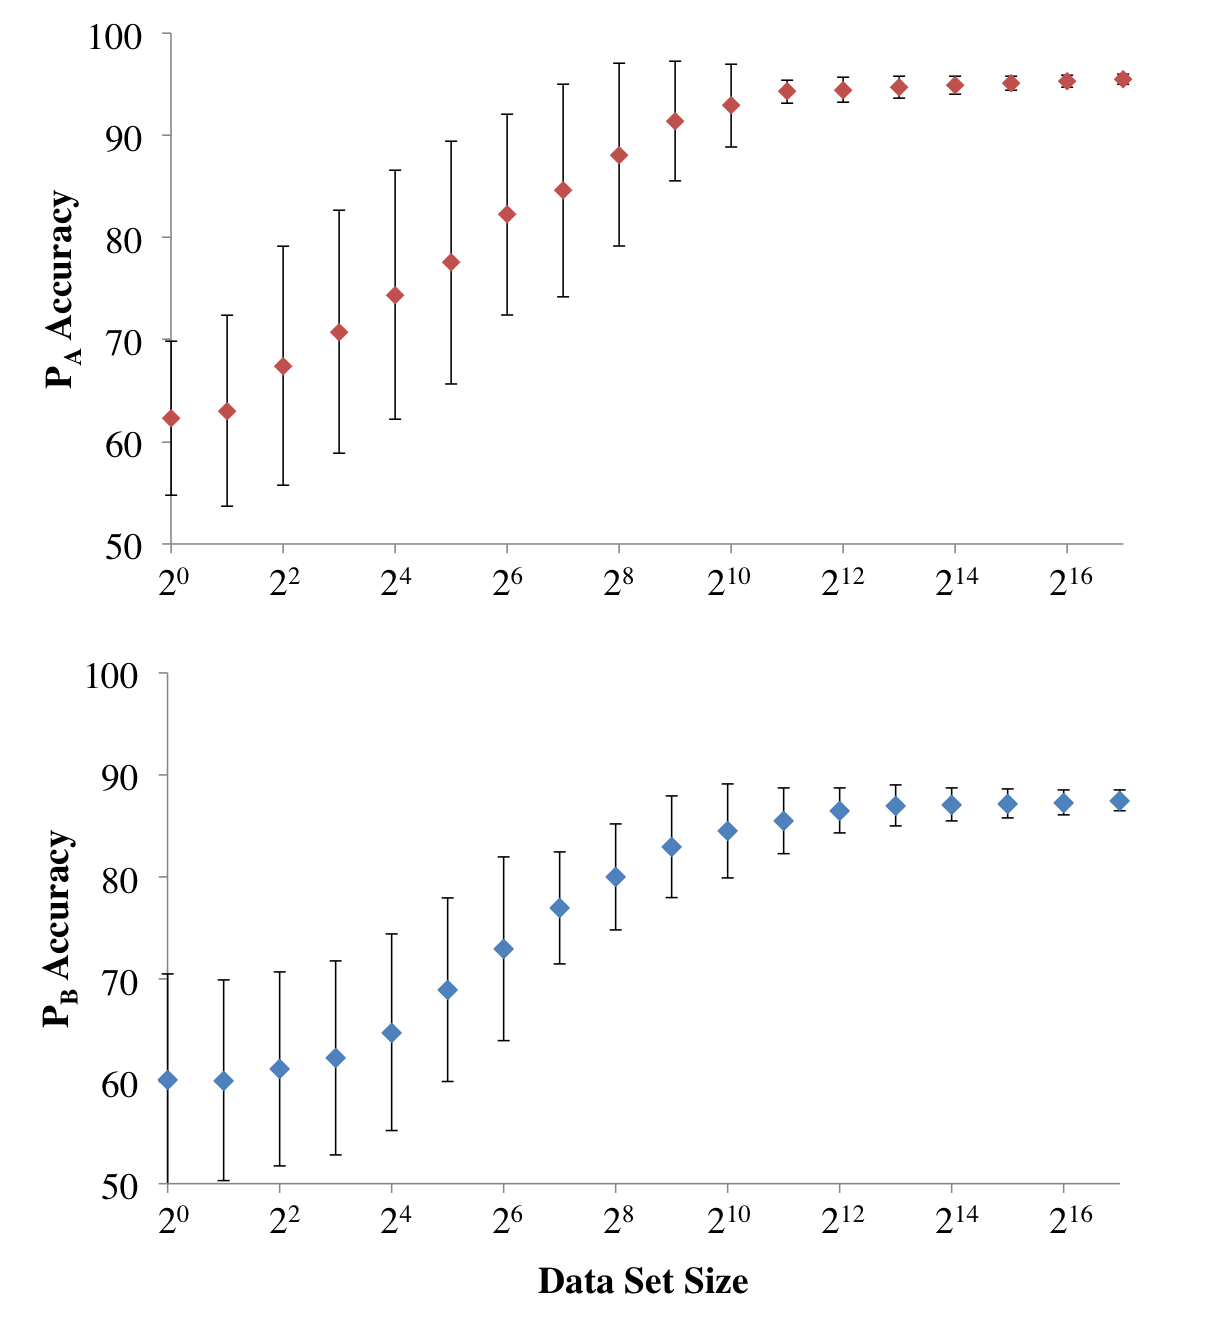
\includegraphics[width=0.5\columnwidth]{img/lcs}
\caption[Poison path learning curve]{Learning curve for \Pa (above) and \Pb (bellow). Students are subsampled randomly from dataset. Error bars are standard error.}
\label{fig:learningCurve}
\end{figure}


While the Rivers Policy performed well on the \Pb in many instances in \Pa it would suggest a student undo something constructive from their partial solution. The optimal static analysis algorithm was worse than the best trajectory based algorithm and it would have been very difficult to design such a system for \Pb\hspace{-0.5mm}. There is a lot of nuance that goes into deciding what a student should do. The experts seem to be working in a formulaic way, but it is very difficult to codify their decision making. 

There are several variations of the Poisson Path that we tested to understand what preprocessing was most important. The two steps that were necessary were: (1) interpolate each student series over the graph of single legal moves and (2) condition node counts on success (see table \ref{tab:results1}). Removing cycles from student partial solution series is less important. We applied the same pre-processing for all algorithms tested.

We ran an experiment to understand the effect of dataset size on accuracy. On both \Pa and \Pb we subsampled students from our dataset and reran the entire policy learning process (including the interpolation). The policy generated by the subsampled students was evaluated for accuracy on the same gold standard expert data. We started with a training dataset size of two students and continually doubled the number of students. For each size we repeated the experiment 100 times to estimate accuracy mean and standard deviation.  See figure \ref{fig:learningCurve}. Even if we were given historical data from substantially fewer students the Poisson Path PSP would have had comparable accuracy. With a dataset of only two thousand students accuracy is similar to the results from running the algorithm on hundreds of thousands of students. While two thousand students may be sufficient, as more data is collected the algorithm monotonically improves in accuracy and accuracy variance. Since the Poison Path algorithm can be cast as an instance of Dijkstra's shortest path the running time will be reasonable even for courses that are orders of magnitude larger than the Hour of Code.



\subsection{Summative Assessment}

\begin{figure*}[!ht]
\begin{center}
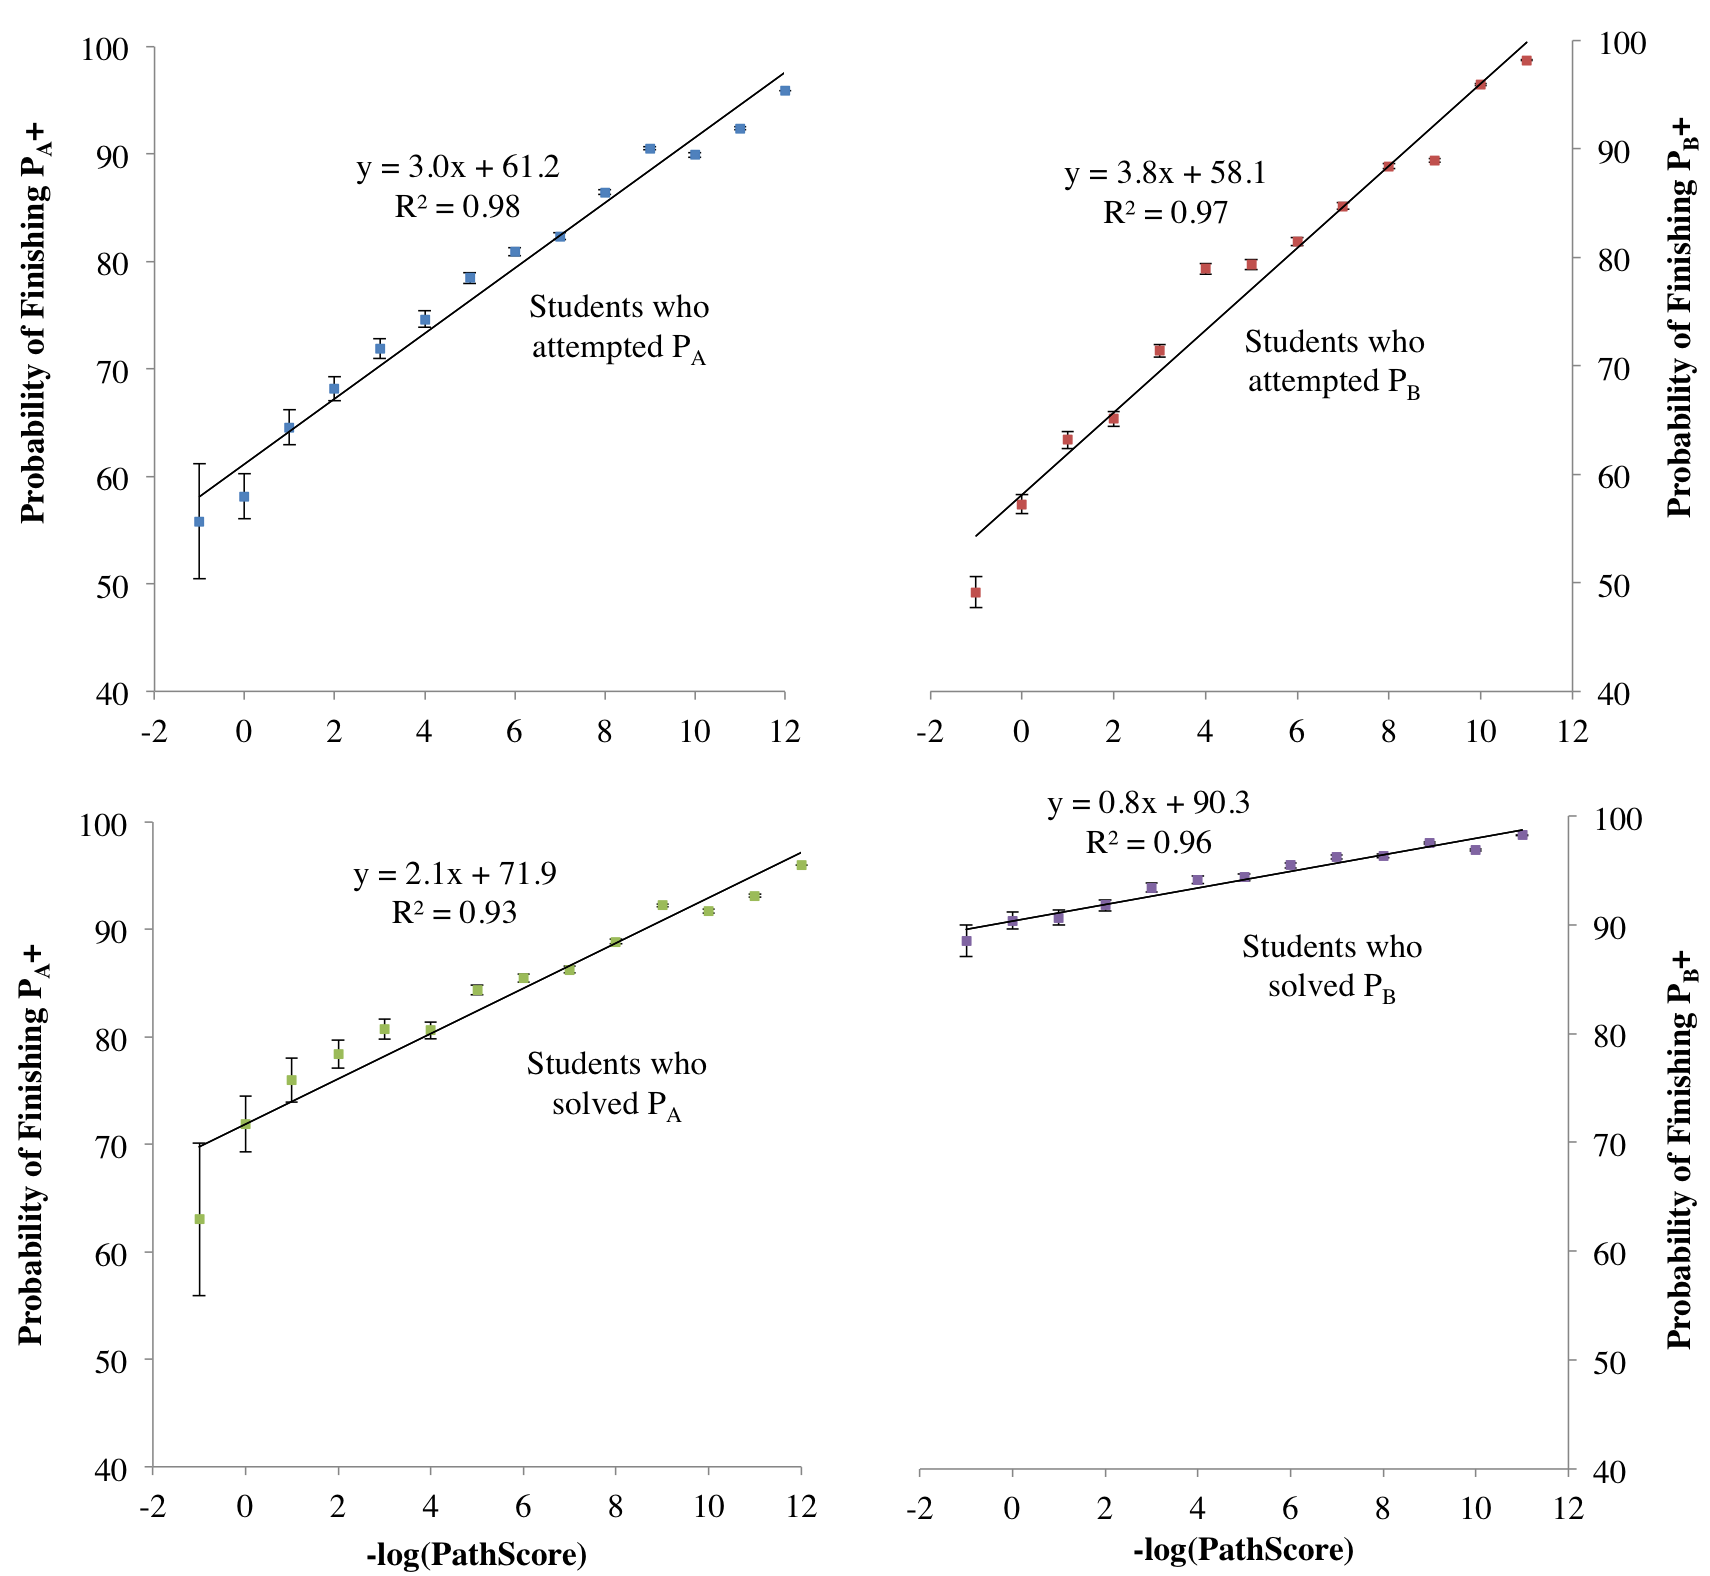
\includegraphics[width=1.0\textwidth]{img/future}

\end{center}
\caption[Poisson path score predicts completion]{Student path scores vs probability of completion of subsequent problems. Error bars are standard error.
 }
\label{fig:predacc}
\end{figure*}

The same insights that allow us to predict how experts would suggest students make forward progress can be used to understand how well each student progressed through the assignment. The desirable path theory that inspired both the Poisson Path and the Independent Probable Path algorithms suggests a statistic that can be measured per student. Assuming that path counts of a partial solution are a function of desirability, we can then calculate the desirability of the path of partial solutions a student took through as they worked through a challenge. 

Based on the Poisson interpretation of desirability used in the Poisson Path, we define the ``path score" of a student's series $T$ to be the time we expect an average successful student would take to complete the series. Assuming that each state is generated via a Poisson process, expected time until we see the series of states that constitute a path is the sum of the inverse of the rate of each partial solution:
\begin{align*}
 pathScore(T) = \sum_{x \in T}{\frac{1}{\lambda_x}}
\end{align*}
 We calculated the path score for each student and explored how the scores were related to the probability that the student would complete the next challenge. For example \Pa is the fourth challenge in the Hour of Code. We computed a path score for each student that completed \Pa and observed which of those students went on to solve the fifth challenge (\Pa+).



From simple visualization it was clear that the negative log of the path score had a strong linear relationship with probability of completing the next challenge for students in both \Pa and \Pb\hspace{-0.5mm}. For the population of students who attempted \Pa, their probability of completing the next challenge \Pa\hspace{-0.5mm}+ increased by 3\% with each per unit increase in $-\log(pathScore)$. Linear regression between $\log(pathScore)$ and the probability of completing the next challenge had an $R^2$ of 0.98. Learners with the worst paths had a 58\% chance of completing the next problem and learners with the best paths had a 95\% chance: an effect size of 37pp. \Pb similarly had an straight line pattern ($R^2$ = 0.97) and an effect size of 43pp. See figure \ref{fig:predacc}.

This trend is especially interesting when we only look at the scores of students who arrived at a solution to the challenge from which we calculate the path scores. These are the students who, if it were a traditional classroom, would have received a perfect grade. For \Pa the successful students with the worst and the best path scores had a 25.1pp difference in the probability of completing the subsequent problem. Again there was a linear relationship between the negative log of the path score and probability of success ($R^2$ = 0.93). \Pb also had a linear relationship ($R^2$ = 0.96), with an effect size that was 9.7pp between the best and the worst path scores. It seems plausible that many students who may have disengaged from the curriculum because of a factor related to low path score may not have stayed in the course until the 18th challenge. In both problems the Path Score shows predictive signal towards retention beyond what we could know from simply observing whether a students solved the challenge.

\subsection{Generating Hints}

In the introduction of this paper we proposed that the challenge of autonomously providing hints could be decoupled into (1) Deciding how a learner should make forward progress and (2) Choosing how to communicate that information to the student such that they improve on a learning objective. Given that we can solve the first task sufficiently well, we are  pursuing research on the second: how to turn our PSP into hints. This latter task combines education and UI decisions.

Having a PSP for a given challenge substantially simplifies the task of generating hints. It tells the hint generation algorithm which part of a student's current partial solution they should work on, and how they should modify their work. Often, students have multiple issues. A policy allows an automated system to know what is the first issue the student should work on. Moreover, knowing the exact edit we believe an expert would like a student to make means that generating a hint is reduced to deciding how directly we should tell the student what to do. Based off of a simple template we turned $\pi(x)$ into English text hints. 

\section{Discussion}

One of the more surprising results of this research is that even with hundreds of thousands of students, it turns out that many reasonable statistics on learner trajectories are not particularly useful for predicting what experts say is the correct way forward. Most interestingly, the transitions that learners take after encountering a problem do not tend to correspond with what experts think learners should do. The wisdom of the crowd of learners, as seen from this angle, is not especially wise. This result raises the question: What is so good about the Poisson Path? Why does it, and the Independent Probable Path work when other methods do not? In designing both of the Desirable Path Algorithms, we followed our intuition that a useful algorithm would be able to predict what an \emph{average} successful student would do if we were to place her in a partial solution. We first assumed that partial solution submission counts are uniquely important as they are a statistic which reflects how desirable a partial solution is to the \emph{average} student (or rather the inverse is a measure of how relatively undesirable). Many baseline algorithms instead relied on transition counts, but that number captures what the biased population of students who had arrived at a given partial solution, \emph{not} the average student, would do. Previous research suggests that transition-based algorithms are limited by lack of data. We now believe that their shortcomings are instead a result of reliance on subpopulations with systematic predispositions. When designing the Desirable Path Algorithms we also assumed that when deciding on a next step it is best to search for an entire path to solution. Many baseline algorithms only consider neighboring partial solutions and do not see the bigger picture. We propose that the success of the Desirable Path Algorithms is evidence that both assumptions are important, operable properties of historical student trajectories. 

Code.org is a compelling case study as tens of millions of students are expected to use the website next year. However, it is only one course and as such is not a proof of our ability to provide feedback for general richly-structured assignments. Even for the Hour of Code where the problems are simple and there are huge numbers of students, the solution space is almost too disperse for statistical methods. Though there may be millions of students, outside the most common partial solutions there is a sharp drop-off in both the density of students per partial solution, and the proportion of students who took reasonable next steps.  For more complicated programming tasks, or written language tasks, there would be too few students that would submit the same partial solutions \cite{huang2013syntactic}; feedback based on historical patterns over raw partial solutions has its limits. One way in which we could further extend the boundary of assignments for which we could provide at scale feedback using the Desirable Path Algorithms would be to develop a better representation for partial solutions and/or a more intelligent way to find patterns in submissions. In general the AI challenges in education are hard and the field can make faster progress if we decouple the evaluation of machine learning tasks so that we can make progress without continuously paying the heavy cost of user studies.

A limitation of our approach is that it is not clear that students need hints and it is not clear that pushing a student towards the answer is the right objective \cite{roll2014benefits}. A lot of learning happens when we struggle and go off on tangents. In the Code.org context, hints that push students towards the solution are useful because the goal of the Hour of Code is primarily motivation. The course intends to provide learners with an exposure to programming. Being able to give a stuck student a hint is useful for fostering retention and interest in the subject. One way to approach the uncertainty of knowing whether a hint would be useful for a student is through a reinforcement-agent hint-giving system. Such a system would be integrated into the website and would dynamically decide whether to give a hint (and if so, which hint). There are well studied ways to balance the need to explore the impacts of giving different hints to learners at different times, and to exploit what is known to work. 

Beyond the capacity to generate hints, the process of finding signals in historical data has interesting side-products. The most important corollary we presented is that the same intuition that guides generating PSPs can help us understand individual learners and predict retention. Piech et al found prototypical clusters of ways in which students solve problems that were predictive of exam scores \cite{piech2012modeling}. This paper goes beyond that result by calculating a continuous valued path score which can make more fine grained predictions. Our ability to predict both retention and teacher suggestions are results that lend credibility to one another. The Path Score metric has obvious utility as a diagnostic measure that could help identify learners that may need more attention. Of course, knowing that a student has a bad path score does not imply \emph{why} the student has a low probability of completing a subsequent challenge. It is only a correlation. It is not clean why Path Scores and probability of retention are exponentially related. One interpretation is that there is a monotonic ability scale and that each unit decrease in ability has compounding, and therefore exponential, impact on how well a student navigates through partial solutions. 

There are more undiscovered patterns in how students navigate richly-structured assessments. Student trajectories remain a great mystery.

\subsection{Conclusion}

In this paper we explored ways to solve the machine learning question: how can we predict the way a teacher would encourage a student to make forward progress? The ability to make such prediction is useful for generating feedback at scale. We show that in the Code.org case study two algorithms with the same theoretical backing are accurate at recreating expert opinion. These algorithms can be applied to logs of learners working on problems for which there are no expert labels, and will produce an intelligent strategy for what learners ought to do. We then claim that the same theory can be used to calculate a statistic on how well a student navigated the assignment and show that this statistic predicts future retention. The way in which students solve problems is fertile ground for research in learning at scale. Instead of looking solely at a student's final answer, education of the future will take note of the journey the learner took to get there.

While the algorithm that we introduced works well for assignments where there are many more students then there are common partial solutions, it does not do so well, we imagine, when assignments become more complex and the solution space becomes more sparse. In fact, most temporal approaches devolve when applied to sparse solution spaces. In this chapter we treated each unique partial solution independently. However there are clearly common structure among different partial solutions. Being able to better understand the collection of partial solutions for sparse solution spaces is a fundamental question that I believe is a prerequisite to understanding students over time in such settings. Thus the next natural question to ask is: How should we model sparse solution space?

\part{How to Model Sparse Problem Space?}

\chapter{Shared Substructures}
Based on a paper: Scalable Homework Search for Massive Open
Online Programming Courses \\ \emph{International Conference on the World Wide Web 2014.}

\vspace{7mm}

\begin{figure}[h!]
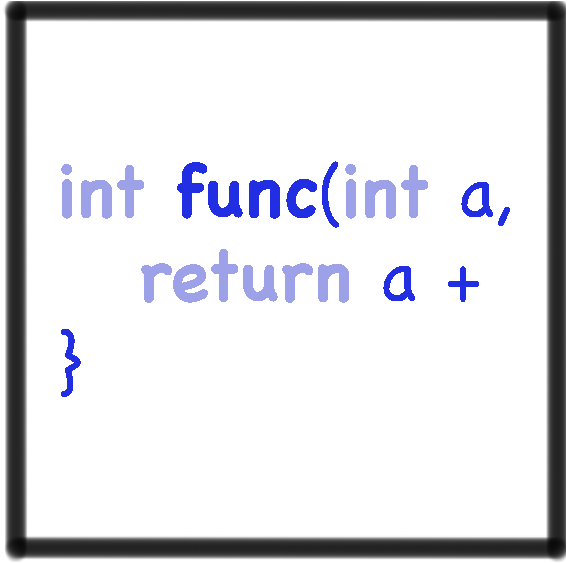
\includegraphics[width=0.2\textwidth]{img/assnType_4}
\end{figure}

\vspace{7mm}

The use of neural networks to learn a joint embedding space is useful for introductory control flow assignments. However for general programs that students would write in an undergraduate programming course, networks which represent recursive structures (such as programs) are currently not powerful enough to be the basis for understanding the space of student partial solutions.

In this chapter we develop a way to understand partial solutions for general programming assignments. To do so we decompose online homework submissions into a vocabulary of ``code phrases'', and based on this vocabulary, we architect a queryable index that allows for fast searches into the massive dataset of student homework submissions. To demonstrate the utility of our homework search engine we index over a million code submissions from users worldwide in Stanford's Machine Learning MOOC and (a) semi-automatically learn shared structure amongst homework submissions and (b)  generate specific feedback for student mistakes. 


\mypara{Search engines for student submitted content}
\looseness -1 %\Chris{This seems to repeat many thoughts from previou sections: 
%There has never existed as pressing a need to efficiently search student online content before.
%But 
With the amount of collected student content increasing at a growing rate
	and the lines between formal classroom learning and informal online learning quickly blurring, 
		search engines for student submitted content seem inevitable, and potentially enormously valuable. 
		%\Chris{this seems like a good place to define what a search engine over homework means. There is a medium intellectual jump between these two sentences}
		These search engines would allow one to explore a massive number of homework submissions by efficiently retrieving submissions matching specific criteria.
Students would then benefit by being able to look for other students who think alike,
			 to see how students with different viewpoints think,
			to find alternative strategies of approaching a homework problem,
			or simply to browse other work for inspiration.
			%\Chris{What about getting feedback? I know its coming... but its not clear here.}
Instructors, on the other hand, would also benefit %, for while an instructor cannot read through tens of thousands
%of student submissions to a MOOC,  she can 
by being able to query a search engine in order to look for submissions of a particular
			type or even to count the number of students who submitted the same
			or a similar class of solutions.
%In this paper, we present a system capable of searching for programming code among a massive collection of submissions to a MOOC. Even though our focus is on code, we believe that similar ideas can have broad impact on a variety of courses beyond computer science.

\looseness -1 While search engines for code have existed for a number of years (see~\cite{paul94,thummalapenta07,hummel08,kim10}),
the nature of MOOC datasets makes for a setting that is quite distinct from that of typical code search.
%Even though one would still need to comb through massive amounts of code, 
In the MOOC setting there is significantly more structure, since
(1)  submissions often take the form of single unit-testable functions written in a single language, and (2) 
all students submit attempts of the same problem at the same time.   
Due to this similarity between many submissions, 
it is possible to exploit the shared structure of multiple submissions in several ways.
For example, this shared structure allows one to reason about the
semantics of code and the intentions of the programmer.   
%\Jon{[DELETE] And of course while it would be nice
%to understand programmer intent in general code, the problem is more important for students who are potentially
%just beginning to learn to code.}


\looseness -1 The engine that we propose in this chapter is built around a massive index over the existing student code submissions
which can be searched using a variety of queries and supports a number of possible applications such as (but not limited to)
finding alternative implementations, mining common approaches and misconceptions, and providing personalized feedback.
%\Jon{Chris?}
Codewebs is designed to be highly scalable, allowing us to
find and leverage shared structure amongst submitted programs and is able to reason about semantically similar student code.
The main power of our system stems from its ability to tailor the way it deals with code semantics to each homework problem individually.
% deals with code semantics is specifically tailored to each homework problem, but 
Specifically, we
utilize existing data to learn about each homework problem rather than requiring an excessive amount of human effort for each problem.
Finally, the Codewebs system is designed so as to be easily portable to diverse programming assignments
and to different programming languages remaining cognizant to the fact that instructor time is a limited resource.
%Our system is 

\mypara{Delivering scalable human feedback}
Instructor time is also a limiting factor in delivering feedback to students, which is critical for learning.
%Another issue in online education that the Codewebs engine addresses is that of allowing a human to scalably deliver feedback.
With the number of engaged students in a MOOC commonly exceeding ten thousand, many benefits of face-to-face instruction are easily lost.
Even despite the fact that programs can be checked for correctness (i.e., unit-tested) automatically, coding assignments are complex in that they can 
be approached with a multitude of algorithms or strategies and typically require creativity. 
Thus in many coding problems, students can benefit from more feedback than a binary ``correct vs. incorrect''.   
It is difficult, however, to gauge student understanding without being able to personally peruse through  tens of thousands of code submissions.
And it is consequently difficult to grade student work, to provide detailed student feedback, or respond to individual questions. 

\looseness -1 Detailed assignment feedback is in general neither easily automated or even appropriate for typical crowd-sourcing platforms such as Mechanical Turk since graders are required to have a certain level of expertise.  One proposed solution (pursued, for example, by the Coursera platform) has been to use peer grading instead, allowing students to grade each other. While peer grading has shown signs of initial success, it also suffers from a number of limitations including inconsistencies and biases amongst peer graders as well as sometimes an unwillingness or inability to provide high quality and constructive feedback \cite{piech13}.

%\looseness -1 Among the many automated and crowdsourcing approaches now available, 
%we take the view that \emph{human instructors still have a key role to play, even in the global classroom}.
%Seamlessly incorporating human feedback into the loop would be both desirable to instructors and beneficial for students.
Our method for providing scalable human feedback derives from the observation that even though there may be many thousands of unique submissions to an open-ended programming assignment the diversity reflects a much smaller number of compounded student-decision points. By recognizing ``shared parts" of student solutions and decoupling different decisions, instructor feedback can be force multiplied. The idea behind our tool is to have an instructor provide detailed feedback only on a handful of submissions which we can intelligently propagate to new solutions via underlying assignment structure learned using our homework search engine. We aim to create a system where a teacher can provide detailed 
feedback for thousands of students with the same effort that she would spend in an ordinary college course.

The strategy of propagating teacher feedback aligns with our view that \emph{human instructors have a key role to play in the future digital classroom}. Seamlessly incorporating human feedback into the loop bridges the gap between the typical MOOC experience and the small classroom experience.
 Finally, because our system discovers the commonalities amongst student submissions using the corpus of students submissions, adding more student data to our data bank
 will improve our statistical confidence and coverage, 
 allowing us to provide meaningful feedback to more students, detect more classes of conceptual errors, and generally improve the utility of our system.

%And by employing the Codewebs engine as a force multiplier, 
%\Jon{We discuss how the Codewebs  engine can  allow for a teacher to provide detailed 
%feedback for thousands of students but with the same effort that she would spend providing 
%feedback to students in an ordinary college course.  In a nutshell, our method works 
%by allowing an instructor to provide
%detailed feedback only on a handful of submissions (or parts of submissions), which we intelligently  propagate to new submissions
%along the ``shared parts'' that the Codewebs system is good at detecting.
%We believe that our system can thus help as a ``force multiplier'' for human instructors who would like to
% bridge the gap between the typical MOOC experience and the small classroom experience. Finally, continually adding student data to our data bank
% will improve statistical confidence and coverage, 
% allowing us to provide meaningful feedback to more students and detect more classes of conceptual errors, and generally improve the utility of our system.}

\mypara{Overview of main contributions}
To summarize, we propose in this paper a novel system, \emph{Codewebs}, for searching through code
submissions to a programming intensive MOOC as well as a methodology for scalably providing
human level feedback to students in the MOOC.
%Our system is fast, makes few assumptions and requires minimal assistance from human instructors.
%More broadly, we believe that search engines for student content are naturally going to be part of the future of
%online learning at scale--and may even be adapted for other web contexts.
%
%\looseness -1 There are several broad technical issues at the core of our system.  First, how to quantify similarity between source code is a notoriously difficult problem.
%In the educational setting, it is particularly crucial to measure similarity not just in syntax, but in semantics and even intention.
%Second, how to seamlessly incorporate human feedback into the loop is desirable to instructors and beneficial for students.
%The final issue is how to scale to courses with  tens of thousands of submissions per programming problem 
%(including indexing and giving of human feedback, and quantifying similarity) --- a problem which will only become
%more difficult as students continue to take the same courses online and as MOOCs become more popular.
%%In this paper we address all of the above issues, proposing highly scalable algorithms for indexing by subtree, subforest, and context, as well as
%%a method for data-driven discovery of  equivalence classes of subtrees/forests which allow users to search for code by semantic similarity.
%%We show that information from a human instructor can be used to facilitate bug understanding as well as to give feedback.
The main technical innovations that we have developed are as follows.
\begin{itemize}
\item We propose an efficient method for indexing code by ``code phrases'' corresponding to constituent parts
of code submissions to a massive scale programming course.  In particular, we introduce a novel way to query for the surroundings, or \emph{context} of a code phrase, 
which allows us to reason about the behavior of code within its context.
\item We develop a data driven approach for automatically finding semantically equivalent code phrases.
In particular we introduce a notion of \emph{probabilistic semantic equivalence} allowing
us to connect syntax with semantics and to compare code with respect to both.
\item We demonstrate applications of our search index
such as bug finding (without having to execute code) and 
allowing a human instructor to  provide feedback at MOOC scales.
\item We demonstrate the scalability of the Codewebs engine and show results on code submissions to a real MOOC, Stanford's machine learning course,
which  had over 120,000 students enrolled worldwide, who submitted over a million code submissions in total.
We also explore the variability of this dataset, showing in particular that the frequency counts of  
student submitted code phrases for a single programming problem follow a Zipf law distribution despite the
fact that all submissions are implementations of the same function.
\end{itemize}
\begin{table}[t!]
\center
\begin{tabular}{|c|c|}
\hline
   \# submissions in total & 1,008,764 \\
   \# coding problems & 42 \\
    Average \# submissions per problem & 24,018 \\
    Average \# students submitting per problem & 15,782 \\
    Average \# of lines per submission  & 16.44 \\     %(discounting starter code)
    Average \# of nodes per AST & 164 \\
%    Fraction of correct submissions & 1 \\
    \hline
\end{tabular}
\caption[Equivalence class dataset summary]{Statistics of the ML class dataset. }
\label{tab:datasetsummary}
\end{table}
\begin{figure*}[t!]
\center
\subfigure[]{
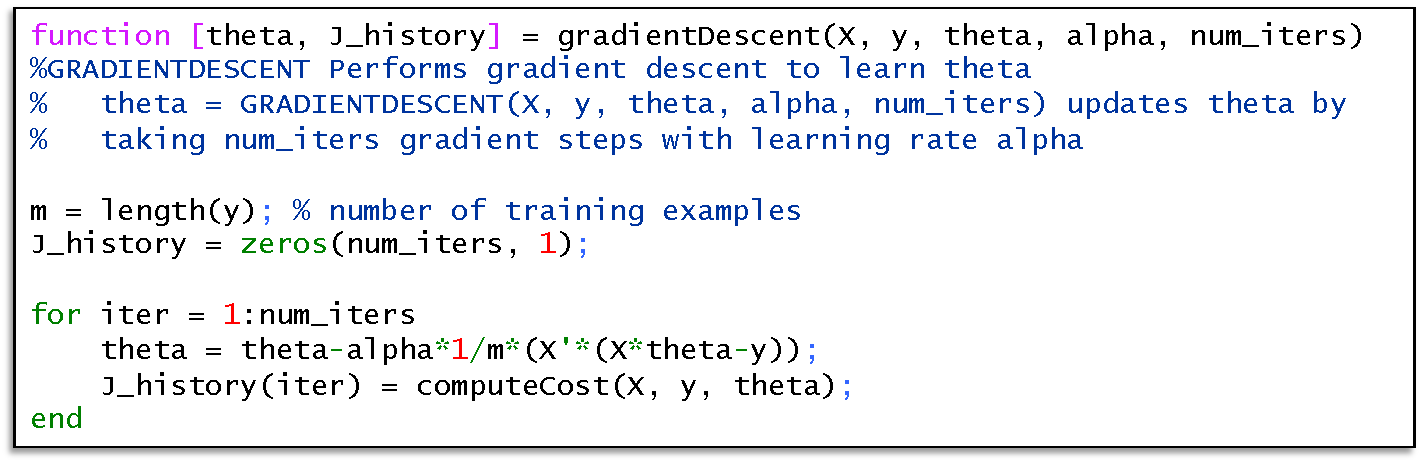
\includegraphics[width=.33\textwidth]{img/goodimplementation.pdf}
\label{fig:codeexample}
}
\subfigure[]{
\raisebox{3mm}{
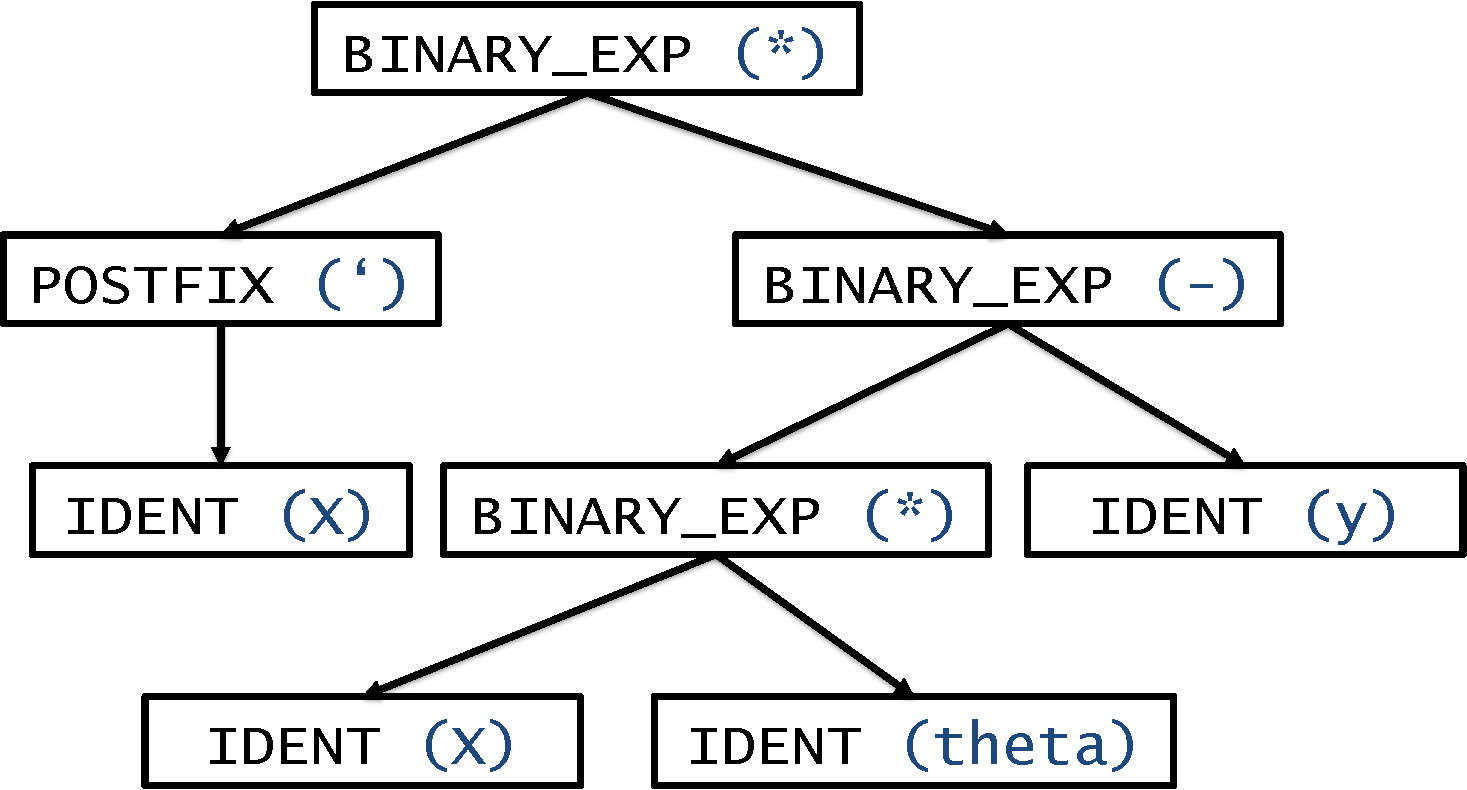
\includegraphics[width=.21\textwidth]{img/astexample2.pdf}
}
\label{fig:astexample2}
}
\subfigure[]{
\raisebox{8mm}{
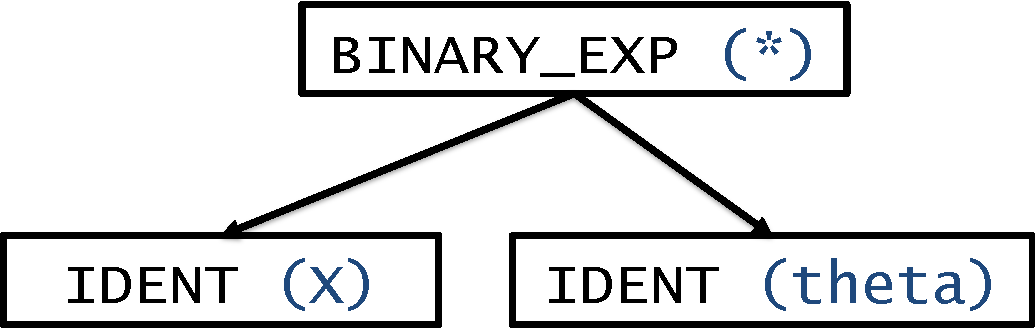
\includegraphics[width=.13\textwidth]{img/subtreeexample.pdf}
}
\label{fig:subtreeexample}
}
\subfigure[]{
\raisebox{3mm}{
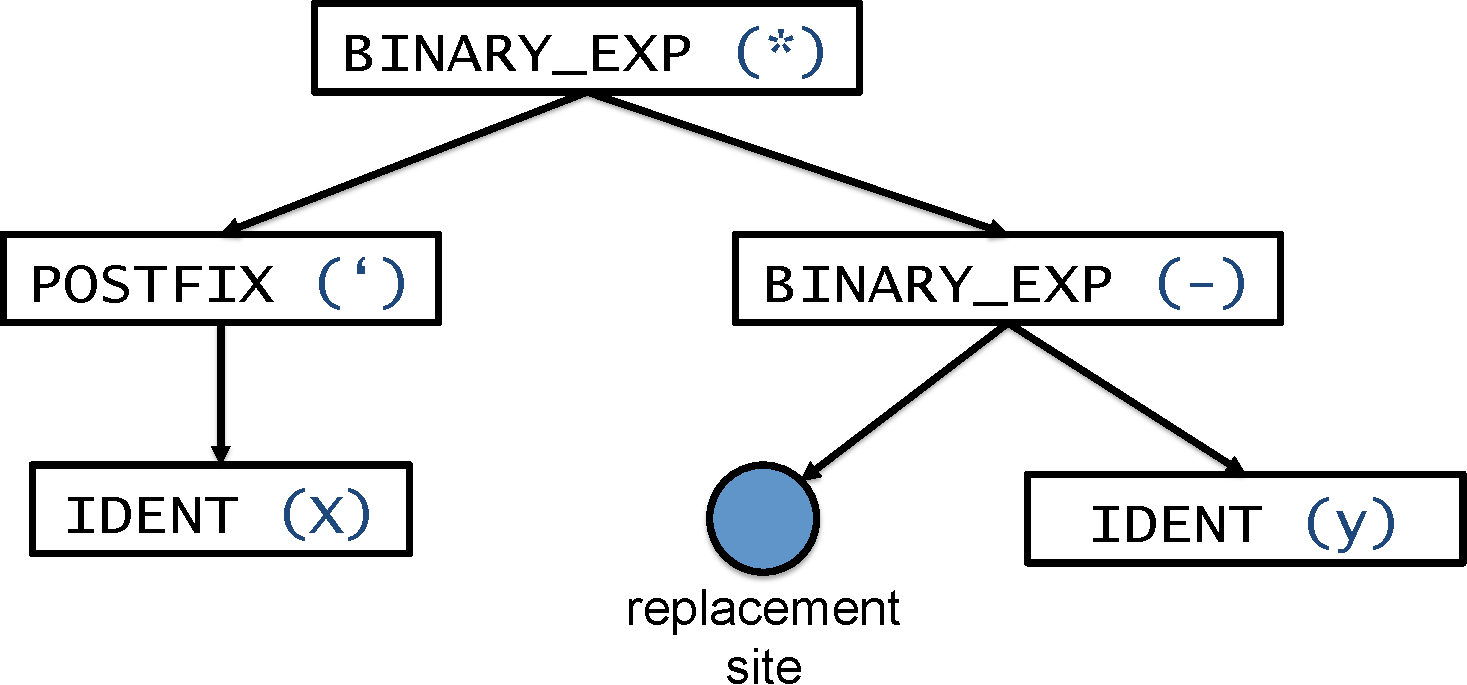
\includegraphics[width=.21\textwidth]{img/contextexample.pdf}
}
\label{fig:contextexample}
}

\caption[Example subtree]{
\subref{fig:codeexample} Example code submission to the ``Gradient descent (for linear regression)'' problem;
\subref{fig:astexample2} Example abstract syntax tree for linear regression gradient expression: $X'*(X*\theta - y)$;
\subref{fig:subtreeexample} Example subtree from the AST from Figure~\ref{fig:astexample2}; \subref{fig:contextexample} 
Context of the subtree with respect to the same AST.  Note the additional node denoting the ``replacement site'' of the context.
}
\end{figure*}



\section{Data from a programming intensive MOOC}\label{sec:dataset}
We showcase our Codewebs system using data collected from 
Stanford's online machine learning (ML) Class (taught by Andrew Ng), 
which opened in October 2011 with over 
120,000 students registering. Over the duration of the course,
over 25,000 students submitted at least one assignment, and 
10,405 students submitted solutions to all 8 homework assignments.  Each
assignment had multiple parts (which combined for a total of 42 
coding problems), in which students were asked to implement algorithms covered in lectures such as regression, neural networks and support vector machines.
Code for the ML class was predominantly written in Octave, a high level interpreted language similar to MATLAB,
and the submissions collectively covered nearly all of Octave's basic language features.
Submissions to the course website were assessed via a battery of unit tests where the student
programs were run with standard input and assessed on whether they produced
the correct output. 
We remark that high level languages such as Octave are fairly popular for instruction because they
allow a student to ignore many of the low level frustrations associated with programming and 
concentrate on the more important higher level concepts.
But they are also harder languages to automatically analyze due to their more flexible syntax and dynamic typing.
As we show in this paper, data driven methods give us a way to effectively analyze submissions in such languages.

\looseness -1 Figure~\ref{fig:codeexample} shows a correct attempt at the ``Gradient descent (for linear regression)'' problem
assigned in the first homework.  In this problem, students were asked to find a linear predictor of the output vector $\texttt{y}$
based on the input matrix $\texttt{X}$. Throughout the paper, we will use this linear regression coding problem as a running example.

\looseness -1 The Codewebs engine allows us to efficiently query this massive collection of code 
submissions from Stanford's ML class, all of which attempt to implement the same functionality.  With so many submissions of the same 
programming problem, we are able to obtain a dense sampling of the solution space, in which 
 we observe almost every conceivable way of approaching the problem both correctly and incorrectly.
The dataset is thus perfect for highlighting the advantages of Codewebs which is able to exploit large amounts of data to do things 
that would be much more difficult to accomplish otherwise.
At the same time, a massive course such as ML class can greatly benefit from a detailed student feedback tool, 
making our dataset also ideal for demonstrating the applicability of Codewebs.
More statistics of our dataset are summarized in Table~\ref{tab:datasetsummary}.

	
\mypara{Structured representations of syntax} 
\looseness -1 In addition to a string representation of each student's code submission,
we parse each student submission into an \emph{abstract syntax tree (AST)} representation. 
Each AST (which is equivalent to that created internally by the Octave software~\cite{eaton97}) 
is stored explicitly in our database in JSON format.   An example AST is depicted in Figure~\ref{fig:astexample2}.
Running on the ML class dataset, our parser accepts over 99.5\% of  submitted code, failing in 
a small percentage of cases (often due to submissions in different languages such as Python or MATLAB),
which we discard from the dataset.  
Nodes in our ASTs are specified by a \emph{type} (e.g., $\nodeSTATEMENT$, $\nodeASSIGN$) and an optional \emph{name} (e.g., $\texttt{X}$, $\texttt{theta}$, 
$\texttt{gradient}$). 
Other than the statement and identifier nodes, we do not assume any specific knowledge of the semantic meanings of node types.

\looseness -1 Reasoning with abstract syntax trees instead of the original source code allows the Codewebs system to effectively ignore
cosmetic idiosyncrasies in whitespace, comments, and to some extent, differences in variable 
names.   We find in many cases that multiple submissions that are distinct as code strings can correspond to the same AST.
Thus after parsing, we retain just over half a million distinct ASTs from the original million submissions along with the number
of occurrences of each unique AST.  

\section{Efficient Indexing of code submissions}\label{sec:indexing}
\looseness -1 What basic queries or items should a code search engine index?
If we viewed code simply as a string, it would be reasonable to query by terms, or phrases or regular expressions,
but with the additional tree structure of our ASTs, we can go beyond traditional ``flat'' queries.
The Codewebs engine accepts basic queries in the form of what we call \emph{code phrases}, subgraphs of an AST
which take three forms: subtrees, subforests, and contexts, which we now define.  In the following, consider any AST denoted by $\AST$:

{{\noindent \bf [Subtrees]}} \emph{Subtrees} represent the most basic form of code phrases and 
are specified by a single node $\node$ in AST $\AST$ and contain all descendants of $\node$.
If an AST $\mathcal{B}$ is a subtree of AST $\AST$, we write $\mathcal{B} \leq \AST$.
When referring to a specific subtree rooted at a node $\node$ of an AST, we write $\subtree$.

{{\noindent \bf [Subforests]}} In addition to subtrees, we consider \emph{subforests} which capture everything in a contiguous sequence of statements.
Specifically, we define a subforest to be a consecutive sequence of \emph{statement subtrees} (i.e., 
subtrees rooted at $\nodeSTATEMENT$ nodes).  

{{\noindent \bf [Context]}} Because the function of a code snippet generally depends strongly on the surrounding region of code in which it appears,
we also allow for these surroundings to be directly queried by our engine. 
Formally, we define the \emph{context} of a subtree $\subtree$ within a larger subtree $\subtreeprime$ of the same AST
to be the subgraph of $\subtreeprime$ which does not contain anything in $\subtree$ to which we add an additional leaf attached to the parent of $\node$,
representing the ``replacement site'' where other subtrees could potentially be swapped in.
For example, the context of the body of a for-loop with respect to the subtree rooted at that for-loop contains a 
variable and expression specifying termination conditions.  We denote the context by $\subtreeprime\backslash\subtree$.
Figure~\ref{fig:subtreeexample} shows an example subtree with its corresponding context (Figure~\ref{fig:contextexample}).
 We also refer to two special types of contexts:
\begin{itemize}
\item Given AST $\AST$  and subtree $\subtree$, 
the \emph{global context} of $\subtree$ with respect 
to $\AST$ (written $\AST\backslash\subtree$) refers to the tree obtained by removing $\subtree$ from $\AST$.
\item Given a subtree $\subtree$ rooted at node $\node$ in AST $\AST$, the \emph{local context} of $\subtree$ with respect to $\AST$ (written $\parentsubtree\backslash\subtree$)
is the context of $\subtree$ within the subtree rooted at $\node$'s parent.
\end{itemize}




\mypara{Building an inverted index}
We now describe the construction of the
inverted index at the heart of the Codewebs system, associating possible code 
phrases of the above three types to lists of ASTs in the database which contain those phrases.  For simplicity, 
we only consider \emph{exact} code phrase matches in this section and defer the general case to Section~\ref{sec:equivalence}.
While traditional search engines \cite{zobel06} typically do not index arbitrarily long phrases, it makes sense in the student code setting to index with respect to
\emph{all} possible code phrases defined above since (1) student code submissions are typically limited in length (see Table~\ref{tab:datasetsummary}), 
and since (2)  virtually all of the submissions attempt to implement the same functionality, resulting in many ASTs sharing large code phrases. 
%\Jon{We might want to introduce notation for ``kth ancestor of a node'', but not clear if it is necessary yet.}

\looseness -1 The inverted index is incrementally constructed by adding one AST at a time as follows.
We first preprocess all ASTs by anonymizing identifiers that are not recognized as reserved Octave 
identifiers or as those belonging to the provided starter code for the assignment.
Then for each AST $\AST$ in the data,
we extract all relevant code phrases by iterating over all subtrees, all consecutive sequences of statements, 
and their respective global contexts. For each code phrase, we append $\AST$ to its corresponding list in the inverted
%and all $k^{th}$-layer contexts for each subtree (and for all possible $k$).  For each code phrase, we append $\AST$ to its corresponding list in the inverted
index (or start a new list containing $\AST$ if the code phrase was not already contained in the index).	
Since we consider all possible code phrases and allow them to be arbitrarily large in size,
na\"{i}vely building the index would be computationally expensive.  In the following, we describe a scalable index
construction algorithm based on an efficient hashing approach.



\subsection{Efficient matching}
Our inverted index is implemented as a hash table.  To efficiently query the index, we compute
hash codes for each code phrase by hashing the list obtained via a postorder traversal of its nodes.
Specifically, given an AST $\AST$ with nodes $\nodeIdx{0},\dots,\nodeIdx{m-1}$ (the postorder of $\AST$),
we hash $\AST$ via the function:
$
H(\AST) =  p^m + \sum_{i=0}^{m-1} p^{m-i-1} h(\nodeIdx{i}), 
$
where $p$ is a prime number and $h(\node)$ can be any hash function encoding the type and name of the node $\node$.
Code phrases (whose nodes can similarly be postordered) are hashed using the same function.
We note that phrases that share the same postorder (despite being structurally distinct) are guaranteed to collide under $H$, but 
in practice, we find that it works sufficiently well (perhaps because it is unlikely for two distinct ASTs to simultaneously meet
the constraints of sharing a postorder traversal and corresponding to valid source code).

%We define the hash of the replacement node for contexts
%to be 1. 


\mypara{Efficient precomputation of hashes}
\looseness -1 By exploiting the particular structure of the hash function $H$, we can efficiently precompute
hash codes for all code phrases within an AST.
We explicitly maintain  a serialized representation of each AST $\AST$ in our dataset
as a flat array $L_\AST=[[{\bf\ell_1},\dots,{\bf\ell_m}]]$ 
where the $i^{th}$ entry of $L$ corresponds to the $i^{th}$ node ($\nodeIdx{i}$) of the postorder of $\AST$.
We record node type and name in each entry $\entryIdx{i}$ as
well as the size (i.e., number of nodes) of the subtree $\subtreeIdx{i}$ (which we denote by $|\subtreeIdx{i}|$).
Note that with size information,  the original AST is uniquely determined by the flat array of nodes (and it is thus possible
to check for \emph{exact} matches between ASTs), but we ignore sizes during hashing.
%}
%The advantage of this serialized representation is that each of the possible code phrases defined above can 
%similarly be represented and constructed efficientl

The advantage of representing an AST $\AST$ as a serialized list $L_\AST$
is that each of the code phrases appearing in $\AST$ can be similarly represented, and in fact, \emph{directly
constructed as a contiguous subsequence} of entries of $L_\AST$.
%In particular, the subtree rooted at a node $X$ corresponds to the the contiguous sequence between
In particular, the subtree $\subtreeIdx{i}$ corresponds precisely to the nodes in 
the contiguous subsequence: $[[\entryIdx{i - |\subtreeIdx{i}| + 1},\dots,\entryIdx{i}]]$.
Serialized representations of subforests similarly correspond to contiguous subsequences of $L_\AST$.
%Since we constrain subforests to be the union of subtrees rooted at consecutive statement nodes, 
%subforests are also guaranteed to correspond to a contiguous subsequence of the form $[[\entryIdx{j_{low}},\dots,\entryIdx{j_{high}}]]$,
%where $j_{low}$ and $h_{high}$ are the lowest and highest post-order indices in the subforest, respectively.
Obtaining a serialized representation of a context is only slightly more complicated.  Given the context  $\subtreeprime\backslash\subtree$,
we take the subsequence of $L_\AST$ corresponding to the larger subtree $\subtreeprime$ but replace the entries corresponding to the smaller subtree $\subtree$
with a single entry denoting the replacement site node.

Together with the simple additive structure of our hash function $H$, the fact that all code phrases can be read off as contiguous subsequences, 
lends itself to a simple dynamic programming approach for precomputing all code phrase hashes of an AST in a single pass.
Specifically, if we store the hashes of all prefixes of the postorder list (as well as all relevant powers 
of the prime used in the hash), we can compute the hash of any sublist in constant time, with:

{\scriptsize
\[
H([[\entryIdx{i},\dots,\entryIdx{j}]]) =  H([[\entryIdx{0},\dots,\entryIdx{j}]]) - p^{j-i+1} (H([[\entryIdx{0},\dots,\entryIdx{i-1}]]) - 1).
\]
}

\noindent Since every code phrase contains at most two sublists from the postorder of the
original AST, the hash for each code phrase can be computed in constant time using $O(m)$ precomputation time and additional storage.
%\Jon{we need to have at least one sentence about quadratic scaling with number of statements in the function}
%\Jon{this part might need a diagram}
%\mypara{Index storage requirements}
%Again, since every code phrase contains at most two sublists from the postorder of the original AST, 
The same reasoning allows us to represent each
code phrase as a view into subregions of the original AST.  
Thus we only require a constant amount of additional storage per code phrase.




\section{Data driven discovery of semantic equivalence classes}\label{sec:equivalence}
One of the main difficulties in matching source code  is that there are  
always many syntactically distinct ways of implementing the same functionality. 
For example, where one student might use a for-loop, another might equivalently use a while-loop,
%and De Morgan's laws (and distributive laws in general) can be used to transform
%the apparent syntax of a boolean or algebraic expression.
and if we were to require exact syntactic matches between code phrases (as was assumed in the previous section), we would not be
able to capture the fact that the two submitted implementations were highly similar.

To address the issue of non-exact matches, some authors have turned to a softer notion of matching between ASTs
such as tree edit distance (see \cite{shasha94}). But this approach, which has been used in works on generic
code search as well as tutoring systems \cite{kim10,huang13,rivers13} is based only on syntax
and is not able to directly capture semantic equivalence.
Another more direct approach is to rely on \emph{canonicalization} (\cite{paul94,xu03,rivers12,rivers13}) in which one
applies semantic preserving transformations to the AST in order to reduce it to something more likely to match with other code in the database.
%transforms the AST to forms based on a known set of transformation rules that preserve semantic meaning.
Rivers et al.~\cite{rivers12}, for example, collapse constant functions, and use de Morgan's laws to normalize boolean expressions (among a number of 
other canonicalizations).

While canonicalization can be useful, it is limited by the fact that a set of semantic-preserving AST transformations must be 
specified a priori.  The task of designing transformation rules is highly nontrivial however, and differs for each programming language.
For example, while it is reasonable to canonicalize the order of multiplication between integers in a strongly typed language such as Java, 
it might not be possible under a dynamically typed language such as Octave or Matlab, where the dimensions of a variable are not known until runtime.
Furthermore, canonicalization cannot capture programmer intent --- if a programmer incorrectly writes a code snippet, 
canonicalization might help to group it with other equivalently wrong snippets, but is unable to connect the the incorrect snippet with a correct counterpart.
%First, it doesn�t scale well to lots of classes (lots of programming languages)
%But mostly we think this can only get at a little bit of variance.  
%In general code search settings, you can't possibly write down all the semantically equivalent ways to write down something.
%It is tempting to code basic properties such as associativity of addition or multiplication, but even this can be tricky with dynamically
%typed languages such as octave.
%Another thing - it does not capture programmer intent.  If the programmer wrote something wrong, canonicalization will help to group it
%	with other equivalent wrong ways of writing it, but won't capture the fact that it was meant to mean blah.
%Another thing to do is to look at edit distance between ASTs, but this only focuses on syntax and loses out on any semantic meaning.

Our approach is founded on two main observations for dealing with non-exact matches.   
The first observation is that in the education setting where almost all submissions attempt to implement the same functionality, 
it becomes feasible to design a set of semantics preserving AST transformations that is \emph{customized} to each individual programming problem.
Thus instead of having to invent a set of rules that can apply broadly to all programs, we can imagine designing specific syntax transformations
that are likely to be helpful in reducing the variance of student submissions on each particular problem.
In contrast with compiler optimization,
canonicalization rules in the education setting do not have to be perfect  ---
it would be acceptable to use AST transformations that are valid only for \emph{most} students, perhaps
reflecting common assumptions made about each problem.
Our second observation is that this design task can be automated to a large extent, by mining a large enough dataset of existing student submissions accompanied
by unit test outcomes for each submission.


\begin{example}[$\texttt{length(y)}$ and $\texttt{size(y,1)}$]\label{ex:lengthy}
\looseness -1 As an illustration, consider our running example, the linear regression problem. 
Students were given a function prototype, assuming among other variables,  
that a one-dimensional response vector, $y$, would be passed in as input.
One of the sources of variation in the  problem came from the fact that
$\texttt{length(y)}$ and $\texttt{size(y,1)}$ were both valid and common ways of referring to the number of
elements in $y$ (see for example, the first line under the function definition in Figure~\ref{fig:codeexample}).  
It would be wrong to call the two expressions equivalent since
%These two expressions would not be equivalent according to Definition~\ref{def:exactequivalence}, since
in general, $\texttt{length(y)}$ and $\texttt{size(y,1)}$ can give different results depending on the value of $y$.
Thus, a typical canonicalization approach based on semantics preserving AST transformations would not identify these expressions as being similar.
However, in the particular context of this linear regression problem, the two expressions would have been interchangeable
in nearly all submissions, suggesting our approach (described next) of identifying the two expressions as
being \emph{probabilistically equivalent}, and raises the question of how to discover such identifications from data.
\end{example}

There are two phases of our data driven canonicalization approach. In Section~\ref{sec:testing}, we are given 
two code phrases and asked to determine whether they are semantically equivalent based on data.
We then propose a simple semi-automated method in Section~\ref{sec:reduction} that takes a human specified code phrase and searches the database for all equivalent
ways of writing that code phrase.


\subsection{Testing for semantic equivalence}\label{sec:testing}
In order to define our notion of probabilistic equivalence, we first state a formal definition of \emph{exact} equivalence.
We focus on semantics preserving AST transformations which take a subtree (or subforest) and replace it by another.
A reasonable definition might then be as follows. 
\begin{defn}\label{def:exactequivalence}
Given two subtrees (or subforests) $\mathcal{B}$ and $\mathcal{B}'$,
we say that $\mathcal{B}$ and $\mathcal{B}'$ are equivalent if for every AST containing $\mathcal{B}$,
replacing $\mathcal{B}$ by $\mathcal{B}'$ always
yields a program that runs identically (i.e. always produces the same output given the same input).  
\end{defn}
For brevity, we will use subtrees to refer to both subtrees and subforests in the remainder of the section.
Definition~\ref{def:exactequivalence} is a strict notion that might be useful in AST transformations for compiler optimization 
(for example, to replace a for-loop by an unrolled version), but as discussed above, does not capture the notion of
similarity in Example~\ref{ex:lengthy} and is thus overly rigid for our purposes.

\mypara{Probabilistic formulation of semantic equivalence}
We relax two aspects of the definition of exact equivalence:
\begin{itemize}
\item First, instead of asking $\mathcal{B}$ and $\mathcal{B}$' to result in identical behavior under \emph{all} inputs, we ask for 
identical behavior only on a collection of unit tests (which may not be exhaustive in practice), allowing us to verify similarity using data 
rather than having to establish formal proofs about program behavior.
\item Second, instead of requiring that $\mathcal{B}$ and $\mathcal{B}$'  behave similarly under all containing ASTs, 
we only require that the two subtrees behave similarly in the context of ASTs that have a high enough probability of being submitted to a particular problem.	
\end{itemize}
Formally, let $F[\AST]$ denote the output of an AST $\AST$ given a battery of unit tests as input.
In the following, we let $P$ be the distribution over ASTs that could be submitted to a particular problem.
We assume that $P$ exists, but that we only have access to draws from it (the already submitted code).
The hope is that reasoning with $P$ allows us to focus our efforts on the more common solutions and to generalize 
about equivalences to never-before-seen ASTs.  Our relaxed notion of equivalence is as follows:
%The hope is that we can use probabilistic reasoning to generalize to contexts that we may not have seen before.
%Multiple ASTs are assumed in the following to be drawn independently from $P$.

%we allow abstract syntax trees that correspond to no legitimate source code to be evaluated
%under F and assume that it outputs an error code.

%What the strict definition of equivalence fails to capture are all the additional things that we might 
%consider as equivalent in the context of a particular homework problem.  For example,
%in the homework, if $A$ and $B$ are matrices, then we might want to know that $A^T\cdot B^T = (B\cdot A)^T$.
%
%So now given two AST subtrees $t$ and $t'$, let's now consider how we might define $t$ and $t'$ to be ``analogous'' with respect to our dataset.

%\Jon{introduce a context dependent equivalence}
%\Jon{and a context free equivalence}

\begin{defn}\label{def:equivalence}
We say that the AST subtrees $\mathcal{B}$ and $\mathcal{B}$' are $\alpha$-equivalent if, whenever $\AST\sim P$, $\AST'\sim P$, the following condition is satisfied:

{\scriptsize
\begin{equation}\label{eqn:def1}
P(F[\AST] = F[\AST'] \,|\, \mathcal{B}\leq \AST, \mathcal{B}' \leq \AST', \AST\backslash \mathcal{B} = \AST'\backslash \mathcal{B}') \;\geq\; \alpha.
\end{equation}
}

We refer to the above probability as the \emph{semantic equivalence probability}.
\end{defn}
In other words, if we condition two random ASTs  ($\AST$ and $\AST'$) drawn from the distribution $P$ to (1) contain the subtrees
$\mathcal{B}$ and $\mathcal{B}'$ respectively, and (2) agree on global context ($\AST\backslash \mathcal{B}=\AST'\backslash \mathcal{B}'$), 
then the probability that the unit
test outputs of $\AST$ and $\AST'$ agree should be high if $\mathcal{B}$ and $\mathcal{B}'$ are semantically equivalent.


%Returning to Example~\ref{ex:lengthy}, 
%The idea here is that on some contexts, the two subtrees might not actually result in the same output, but most of the time, they do.
%For example, if we assume that $\alpha$ and $\beta$ are scalars in an assignment.
%Then it might be that $\alpha*\beta$ is ``swappable'' with $\beta*\alpha$ under most conditions.
%However, if a user happens to redefine $\alpha$ and $\beta$ as matrices at some point in the code,
%then the commutativity is broken under that particular context.  As long as this mistake
%does not happen too much however, we might still recover that $\alpha*\beta$ is analogous to $\beta*\alpha$
%under our Definition 1.

\begin{figure}
\begin{center}
\begin{algorithm2e}[H]
{\bf function} {\sc EquivalenceProb}\xspace(Subtrees $\mathcal{B}$, $\mathcal{B}'$): \\ 
\mbox{}\\
\ $L \leftarrow \texttt{QueryIndex}(\mathcal{B})$ \;
\ $L' \leftarrow \texttt{QueryIndex}(\mathcal{B'})$ \;
%\ $\texttt{contexts} \leftarrow \{ \AST'\backslash\mathcal{B}'\;:\;\AST' \in L'\}$ \;
%\ Initialize empty hash table $T$ \;
%\ \For{each $(\AST_i,c_i)$ in $L$}{Append $(\AST_i,c_i)$ to $T[h(\AST_i\backslash \mathcal{B})]$ }
%\ \For{each $(\AST_i',c_i')$ in $L'$}{Append $(\AST_i',c_i')$ to $T[h(\AST_i'\backslash \mathcal{B}')]$ }
\ Initialize $\texttt{count}$ and $\texttt{denominator}$ to 0\;
\ $Z \leftarrow 0$\;
%\ForEach{pair $((\AST_i,c_i) \in L,(\AST_i' ,c_i')\in L')$}{ 
\ForEach{AST $\AST_i \in L$}{ 
	\If{$\AST_i\backslash \mathcal{B} = \AST_i'\backslash \mathcal{B}'$ for some $\AST_i'\in L'$}{
	%\If{$\AST_i\backslash \mathcal{B} \in \mbox{$\texttt{contexts}$}$}{
	%\If{$\AST\backslash \mathcal{B} =\AST'\backslash \mathcal{B}'$ \tcp{context matching}}{
\	$w_i \leftarrow c_i*c_i'$ \;
\	$\texttt{count} \leftarrow \texttt{count} + w_i$ if $F[\AST_i]=F[\AST_i']$ \;
\	$\texttt{denominator} \leftarrow \texttt{denominator} + w $ \;
	}
}
\ \Return $\texttt{count}/\texttt{denominator}$ \;
\caption[Algorithm for estimating semantic equivalence]{Pseudocode for estimating the semantic equivalence probability between two subtrees, $\mathcal{B}$ and $\mathcal{B}'$.  
The function $\texttt{QueryIndex}(\mathcal{B})$ is assumed to return a list of pairs $(\AST_i,c_i)$ such that each $\AST_i$ contains $\mathcal{B}$
and $c_i$ is the number of submissions matching $\AST_i$.   Note that the inner loop can be implemented efficiently using 
the precomputed hashes of global contexts (described in Section~\ref{sec:indexing}).
}
\label{alg:estimate}
\end{algorithm2e}
\end{center}
\end{figure}

\mypara{Estimating the semantic equivalence probability}
\mbox{}
Given two subtrees $\mathcal{B}$ and $\mathcal{B}'$, we can now estimate the probability
that the two are semantically equivalent.   Our method relies on querying the Codewebs index, and 
we assume queries always return a list of unique ASTs matching a given code phrase, along with a count of the number of submissions 
matching each AST.
First, Equation~\ref{eqn:def1} can be written equivalently as:

{\scriptsize
\begin{align}
P(&F[\AST] = F[\AST'] \,|\, \mathcal{B}\leq \AST, \mathcal{B}' \leq \AST', \AST\backslash \mathcal{B} =\AST'\backslash \mathcal{B}')  \\
 &\propto \sum_{\substack{\AST,\AST': \\ \AST\backslash \mathcal{B} = \AST'\backslash\mathcal{B'}}} \mathds{1}\{F[\AST] = F[\AST'] \}  \cdot P(\AST | \mathcal{B}\leq\AST) \cdot P(\AST'|\mathcal{B}'\leq \mathcal{A}) \label{eqn:equiv2}.
 	%&\qquad\qquad\cdot P(\AST,\AST\,|\, \mathcal{B}\in \AST, \mathcal{B}' \in \AST', \AST\backslash \mathcal{B} =\AST'\backslash \mathcal{B}')
\end{align}
}

Estimating Equation~\ref{eqn:equiv2}  by plugging  in empirical distributions for $P(\AST | \mathcal{B}\leq\AST) $ and $P(\AST | \mathcal{B}'\leq\AST')$ 
respectively amounts to summing over pairs of ASTs in the dataset that contain $\mathcal{B}$ and $\mathcal{B}'$, respectively, and match exactly
with respect to global context.
For intuition, Algorithm~\ref{alg:estimate} shows pseudocode for estimating the semantic equivalence
probability for two subtrees using Equation~\ref{eqn:equiv2}.  


\subsection{Semantic equivalence classes and solution space reductions}	\label{sec:reduction}
Having now discussed the problem of verifying semantic equivalence between two given subtrees,
we turn to the problem of discovering groups of subtrees that are equivalent and would be useful for canonicalization.
%We can now explore how to propose candidates for this verification.

To discover candidate equivalence classes, we use a two stage process: in the first stage an instructor annotates a small set of ``seed'' subtrees 
that she believes are semantically meaningful, and in the second stage we algorithmically extract as many semantically equivalent subtrees as possible for each of denoted ``seeds.'' 

The main advantage of this semi-autonomous approach is that it results in named equivalence 
classes (as opposed to anonymous equivalence classes) which can be used to provide non-cryptic feedback. A secondary benefit 
is that it enables a simple and efficient algorithm to extract the most important equivalences in an intelligent order.

As an example, given the AST $\AST$ for the implementation in 
Figure~\ref{fig:codeexample},
 in the first phase an instructor might select the subtree $\mathcal{B}$ corresponding to the expression \texttt{(X * theta - y)} and label it as the ``residual." In the second phase the algorithm would find other equivalent ways to write the residual, such as $\texttt{(theta' * X' - y')'}$.
See Figure~\ref{fig:tagging} for more  examples of code snippets that an instructor might select from the linear
 regression problem.

In phase two, we expand the seed subtrees one at a time to build up an \emph{equivalence class}
of subtrees by iterating the following steps:
%We call the surviving set of subtrees an \emph{equivalence class}.  
%In phase two we expand the seed subtrees one at a time by iterating the following steps:
%\Jon{maybe a visual with triangles representing ASTs?}
%\Jon{confusing subtree/subforests}
		
\begin{figure}[t!]
\center
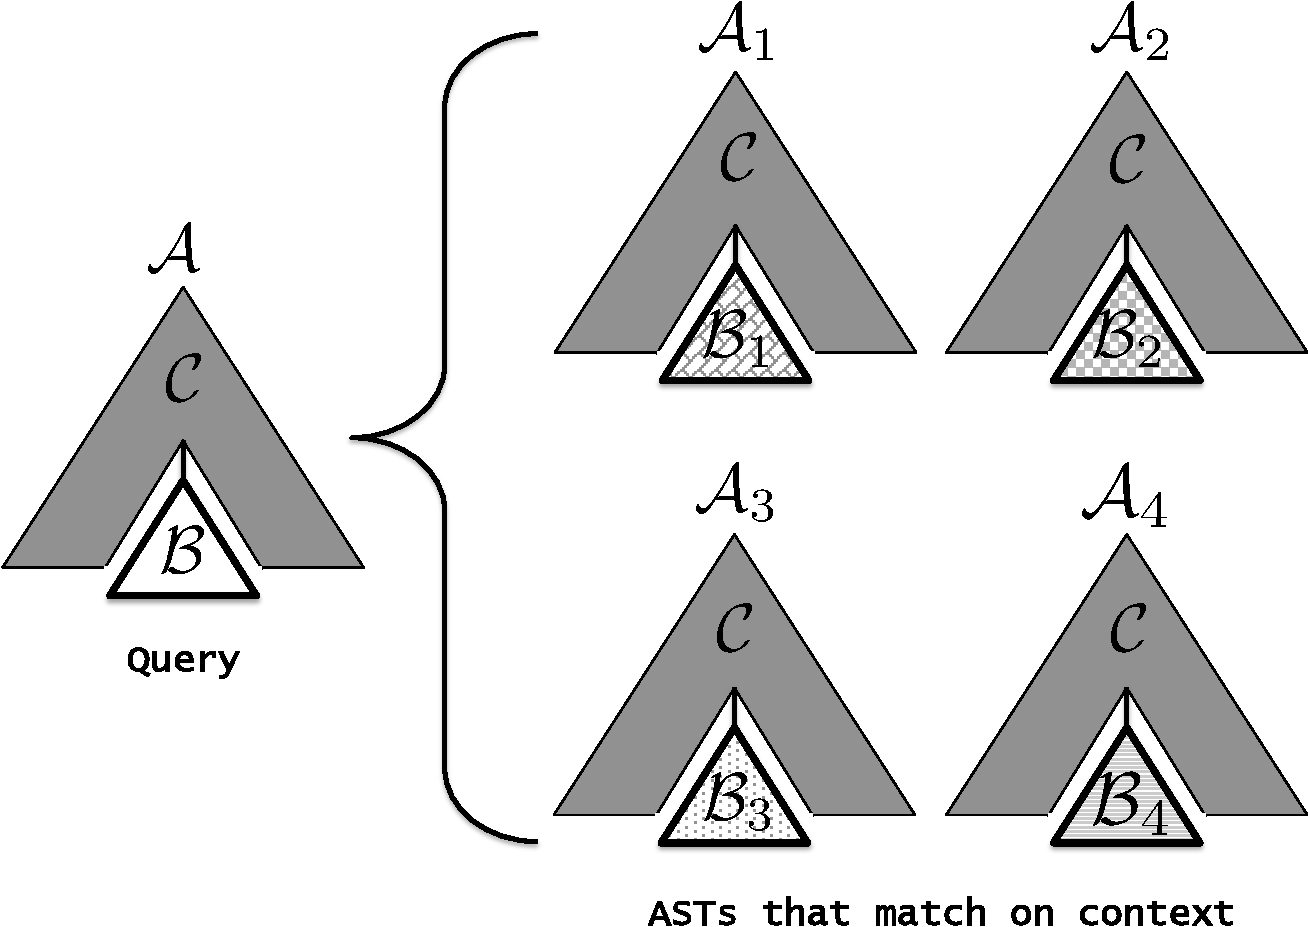
\includegraphics[width=.35\textwidth]{img/cartoon.pdf}
\caption[Equivalence class candidates]{
Given a subtree $\mathcal{B}$ of an AST $\AST$, we query the Codewebs index
for other subtrees that also occur under the same context $(\AST\backslash\mathcal{B})$.
In this case, $\mathcal{B}_1, \dots, \mathcal{B}_4$ would each be considered
as candidates for the equivalence class of subtree $\mathcal{B}$ if the unit test outcomes for their
corresponding submissions matched that of the original AST $\AST$.
}
\label{fig:cartoon}
\end{figure}

\begin{enumerate}
\item {\bf Finding ``feet that fit the shoe''.}
\looseness -1 We perform a first pass to find candidate subtrees that are potentially equivalent to $\mathcal{B}$
by first detaching the subtree $\mathcal{B}$ from its surroundings, leaving the context $\mathcal{C} = \AST\backslash\mathcal{B}$.
We then query our index for the list of ASTs $\{\AST_1,\AST_2,\dots\}$ that contain $\mathcal{C}$ (See Figure~\ref{fig:cartoon}).

Under each retrieved AST $\AST_i$, the subtree $\mathcal{B}_i$ that is attached to the context $\mathcal{C}$ is
then considered to be a candidate for equivalence if $F[\AST_i] = F[\AST]$ (that is, if
the unit test outputs for the containing full AST $\AST_i$ agree with those of the original AST $\AST$). Intuitively, if another subtree shares the context $\mathcal{C}$ and 
produces the same output, it suggests that the two can be interchanged without affecting  functionality.

Before we add a new element to our set of equivalent subtrees 
we use the criterion proposed in Section~\ref{sec:testing} to verify that the new subtree is indeed
probabilistically equivalent to another subtree already in the set.
\item {\bf Finding ``shoes that fit the feet''.}
The first step will find all subtrees that have an exact context match with the originally annotated seed subtree. In order to expand our search for further equivalent subtrees, 
we then search for other contexts that can plausibly be attached to a subtree which is functionally equivalent to the seed. 

For each element $\mathcal{B}'$ in the set of equivalent subtrees found so far, we find all 
contexts that contain  $\mathcal{B}'$ and produce the same output as the program from 
which we found $\mathcal{B}'$. These contexts are hypothesized to also be attached to subtrees equivalent to the seed, 
and as such, represent new places to look for more potentially equivalent subtrees.
 
\item {\bf Repeat Until Convergence.}
We repeat steps (1) and (2) and expand both the set of equivalent subtrees as well as the
set of the contexts that we believe may be attached to one of the equivalent subtrees 
until the size of our set stops growing.
\end{enumerate}

\mypara{Reduction and reindexing}
Each equivalence class
$\Sigma=\{\mathcal{B}_1,\mathcal{B}_2,\dots\}$ 
learned from the data yields a set of canonicalization rules.  Thus whenever
we encounter a subtree $\mathcal{B}$ in an AST which happens to be a member of the equivalence class
$\Sigma$, we can replace $\mathcal{B}$ by a single member of that equivalence class (say, $\mathcal{B}_1$).
The identification of subtrees within an equivalence class
 leads to a reduction in the complexity of the collection of submitted ASTs since ASTs that were previously
distinct can now be transformed into the same tree.  Thus after finding an equivalence class, it is easier to expand a subsequent set.

\begin{figure}[t!]
\center
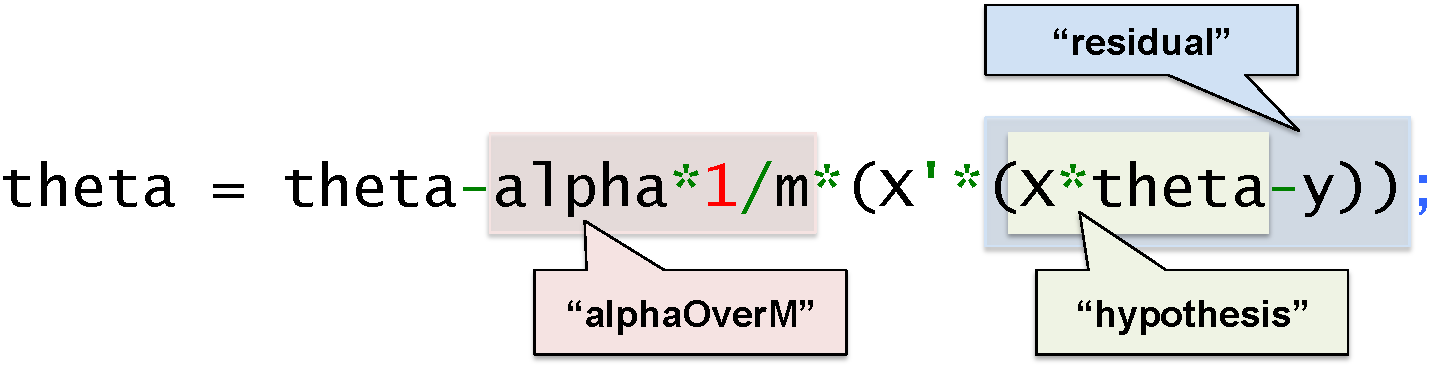
\includegraphics[width=.35\textwidth]{img/taggingexample.pdf}
\caption[Example tagged code]{
Example code snippets corresponding to AST subtrees tagged by an instructor for the linear regression problem.
}
\label{fig:tagging}
\end{figure}

\begin{figure}[t!]
\center
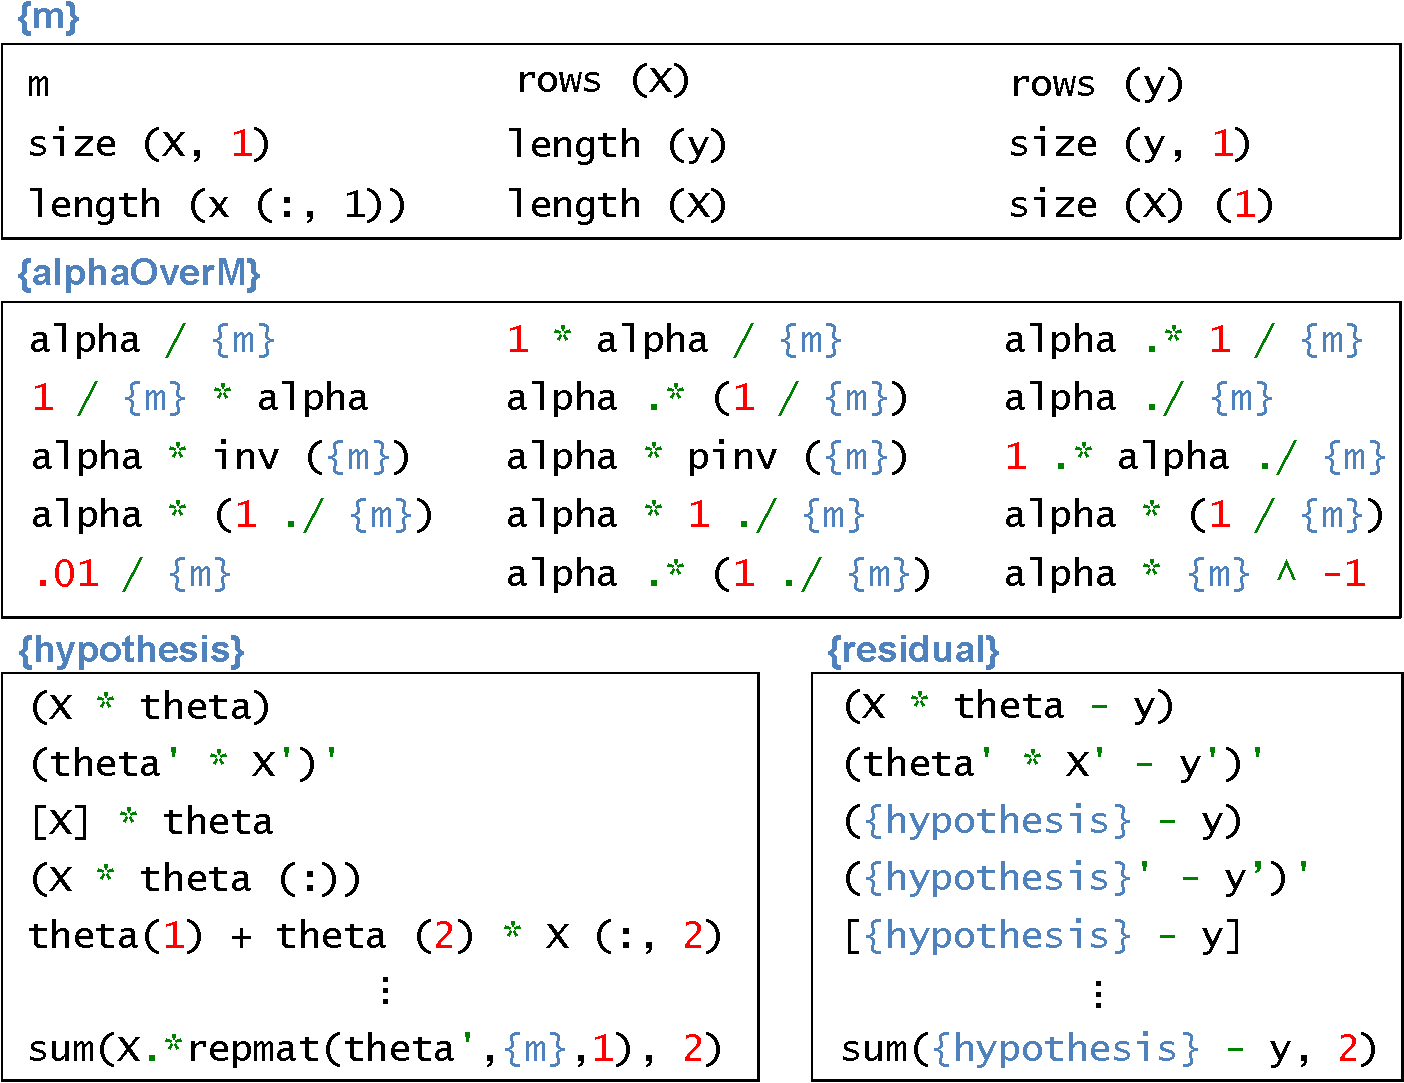
\includegraphics[width=.68\textwidth]{img/equivalencesAll.pdf}

\caption[Resulting equivalence classes]{
 Selections of code snippets algorithmically determined for the linear regression homework.  Note that not all subtrees from the equivalence classes are shown.
}
\label{fig:equivalences}
\end{figure}

\begin{example}
We highlight several examples of equivalence classes that were automatically discovered from the 
submissions to the linear regression problem (shown in Figure~\ref{fig:equivalences} with names in braces).  
Equivalence class $\{m\}$, for example, shows that $\texttt{length(y)}$ and $\texttt{size(y,1)}$ are equivalent, as discussed in Example~\ref{ex:lengthy}.
Note that equivalence classes can be defined in terms of other equivalence classes.

It would be difficult to imagine more than a handful of ways to write the expression $\texttt{alpha/m}$, 
but our algorithm was able to find 135 distinct AST subtrees in the equivalence class $\{\mbox{alphaOverM}\}$.
Note in particular that nearly all of the equivalences 
are not truly semantically equivalent in the strictest sense of Definition~\ref{def:exactequivalence}, but only
in the context of the homework problem.   For example, $\texttt{alpha/m}$ is not interchangeable
with $\texttt{.01/m}$ in general Octave programs, but since $\texttt{alpha}$ was set to be $.01$ for the linear
regression problem, the equivalence was valid in the sense of Definition~\ref{def:equivalence}.
 %Our equivalences do make assumptions which might not always be true even in the context of homework assignments. 
Similarly, we inferred an equivalence between the subtrees $\texttt{inv(m)}$ and $\texttt{1./m}$, which would 
not have been equal if a student had redefined $\texttt{m}$ to be a matrix instead of a scalar.
%The appearance of the subtree $\texttt{(X*theta - y) .* X(:, 1)}$ in Figure~\ref{fig:residual} may seem mysterious --- 
%but it can be explained by the fact that many students assumed the precondition that the first column of the input
%matrix $\texttt{X}$ (i.e., $\texttt{X(:,1)}$), was an all-ones vector (a correct assumption for this particular problem). Discovering these equivalences would be impossible with a small dataset, but with a MOOC-scale dataset, is indeed feasible.
\end{example}


\looseness -1 After the determination of each equivalence class, we rebuild the Codewebs index and optionally
identify further equivalences.  It is often the case that recognizing an equivalence class  $\mathcal{E}$ (and reindexing 
taking $\mathcal{E}$ into account) can help us to discover further equivalence classes.
For example, it might be the case that we do not 
initially have enough observations to conclude with sufficient statistical confidence that 
$\texttt{X*theta-y}$ can be rewritten equivalently as the expression $\texttt{-(y-(theta'*X')')}$.
However, by first identifying that $\texttt{X*theta}$ can be rewritten as $\texttt{(theta'*X')'}$, 
we are likely to find more matches in the database when querying for $\texttt{X*theta-y}$ and $\texttt{-(y-(theta'*X')')}$, respectively,
resulting in a larger sample size from which to draw conclusions.
Using the same insight that we leveraged to find equivalence classes, we can also create a class of \emph{attempts} 
to pair with every equivalence class, where attempts are defined to be
subtrees that fit into the same contexts as members of the equivalence class but change the output from correct to incorrect.
%\Jon{note that collapsing some equivalences can help further ones to be discovered.}

\section{Bug finding from search queries}
Since the input to our system includes unit test outputs, determining whether a code submission contains a bug is not a difficult problem.  However, determining where the bug lies is considerably more challenging.  We discuss a way to use the search engine to localize a bug within code solely by examining its AST.  In the next section we will justify its effectiveness by evaluating its ability to determine the presence of a bug in a query code submission \emph{without} having access to the unit test output of the query.

\mypara{Approach}
As our ultimate goal is to provide useful feedback to as many students as possible, we will focus on common, localizable bugs.  If we consider the distribution of unit test outputs of ASTs which contain a particular subtree, we would expect that such a distribution corresponding to a buggy subtree would be skewed towards incorrect outputs, while that corresponding to a non-buggy subtree would resemble the overall distribution of unit test outputs.  
As long as the subtrees are sufficiently small and the bugs sufficiently common, it is possible to have a reliably large sample of these unit test
output distributions to use for the purposes of classification.

Notice, however, that as the subtrees become larger, the corresponding sample sizes necessarily decrease.  In fact, for any submission not in our training set, the improper subtree consisting of the full AST must has a unit test output distribution with sample size zero.  Thus to increase the sample sizes of our distributions, we use distributions corresponding to local contexts instead of subtrees for classification.

\mypara{Algorithm}
Our algorithm consists of an indexing phase and a query phase.  In the indexing phase, we iterate over the local contexts of all proper subtrees of all ASTs in our collection.  For each unique local context we construct a histogram of the unit tests outputs of the ASTs to which the context belongs.   Notice that these histograms
can be built via queries to our index described in Section~\ref{sec:indexing}.
We then classify each local context as being either buggy or not buggy based on the skew and sample size of its unit test output histogram.

In the query phase, we iterate over the local contexts of all proper subtrees of a query AST.  For each local context $\parentsubtree\backslash\subtree$ we mark node $\parent$ if the local context is recognized as 
buggy by our index.  We then unmark any node with a marked descendant, and report all remaining marked nodes as the roots of the buggy subtrees.

%\subsection{Bug identification by reduction}
%\mypara{Building a bug database}
%\subsection{Statistical bug isolation}

\begin{figure}[t!]
\center
\subfigure[]{
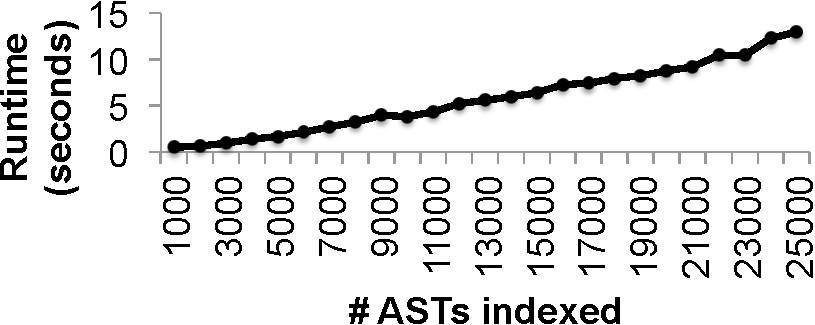
\includegraphics[width=.475\textwidth]{img/numastsvsruntime.pdf}
\label{fig:numastsvsruntime}
}
\subfigure[]{
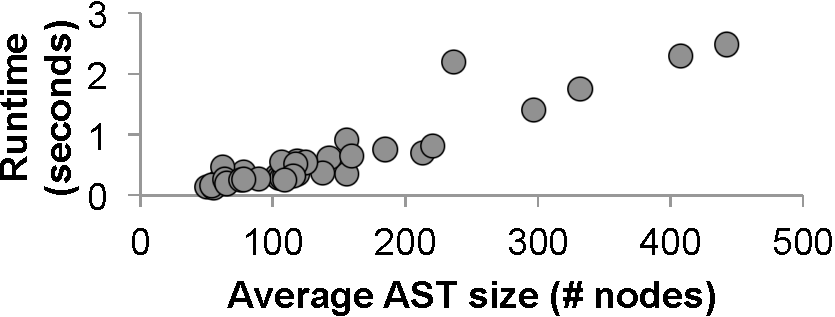
\includegraphics[width=.475\textwidth]{img/astsizevsruntime.pdf}
\label{fig:astsizevsruntime}
}

\caption[Runtime of AST indexing]{\subref{fig:numastsvsruntime} Runtime in seconds for indexing a collection of ASTs (as a function of the number of ASTs)
from the ``gradient descent (for linear regression)'' problem;
\subref{fig:astsizevsruntime} Runtime in seconds for indexing 1000 ASTs from each of the homework problems for Coursera's ML course plotted
against average AST size (\# nodes) for each problem}
%\label{fig:numastsvsruntime}
\end{figure}
\begin{figure*}[t!]
\center
\subfigure[]{
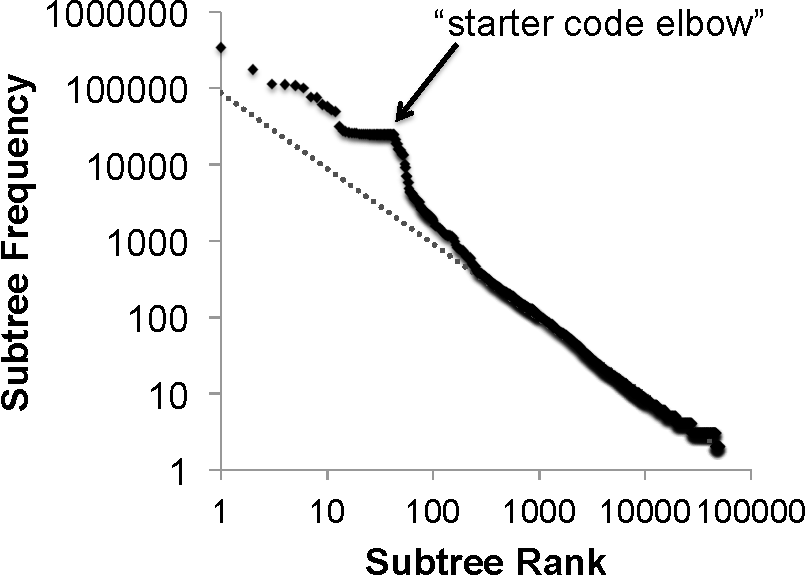
\includegraphics[width=.30\textwidth]{img/zipfnoequivalence.pdf}
\label{fig:zipfnoequiv}
}
\subfigure[]{
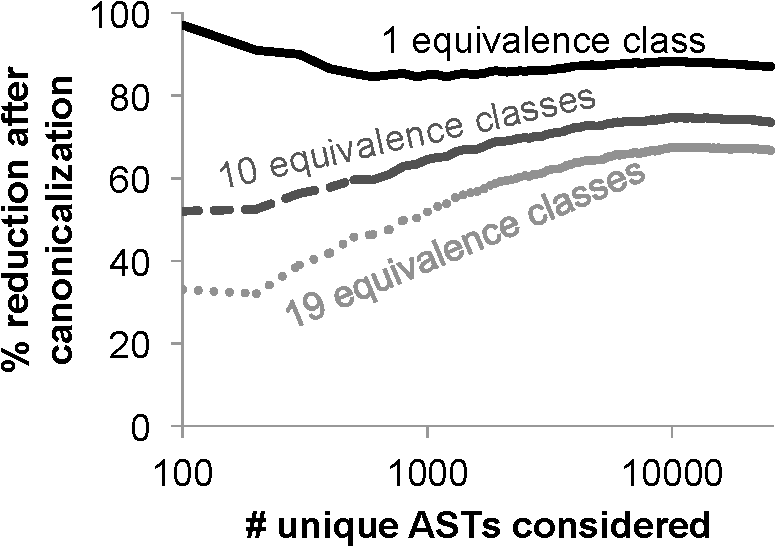
\includegraphics[width=.30\textwidth]{img/reduction.pdf}
\label{fig:reduction}
}
\subfigure[]{
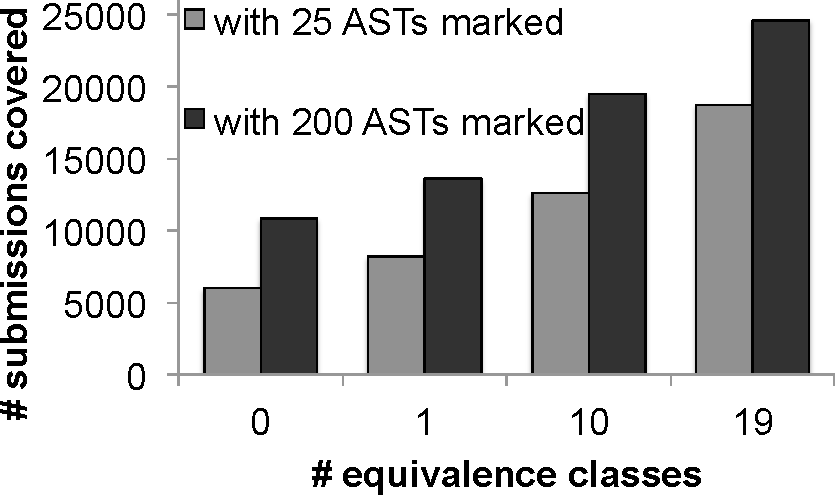
\includegraphics[width=.30\textwidth]{img/reduction2.pdf}
\label{fig:reduction2}
}

\caption[How use of equivalence classes change teacher impact]{
\subref{fig:zipfnoequiv}
Zipf's Law: subtree frequency plotted against subtree rank (in the frequency table). % with and without canonicalization.  
%Note that our data closely follows Zipf's law (dotted line) except at an ``elbow'' at the top of the ranked list.
%We do not include time required for parsing or loading ASTs from disk in the above plot.
%Note that this is eclipsed by time for parsing (roughly 2 hours for all 40790 submissions).
\subref{fig:reduction} Fraction of remaining unique ASTs after canonicalizing the $k$ most frequent ASTs with 1, 10 or 19 learned equivalence classes;
\subref{fig:reduction2} Number of submissions covered if an instructor were to mark the 25 or 200 most frequent ASTs after canonicalization
}

\label{fig:zipfreduction}
\end{figure*}

\section{Empirical findings}\label{sec:evaluation}
In this section we present  empirical studies
of the performance of our Codewebs system and use it to study data from Stanford's ML class.
Our current implementation uses a parser (adapted from the Octave project~\cite{eaton97}) to convert
submitted source code to ASTs.   The Codewebs indexer can be run on a personal
computer with the full index fitting in under 6Gb of main memory for almost all problems.
Our running time tests were run on a %  \Jon{andy's machine}
Lenovo Thinkpad 
%W520 Intel Core i7-2760QM CPU 
(2.40 GHz) with 8 GB RAM.


\mypara{Running time}
We first consider the amount of time required for indexing 
by plotting the running time 
 as a function of the number of ASTs (for the linear regression problem).
We index only the uncanonicalized ASTs for this plot, though in general we iterate through multiple stages of indexing
as new equivalence classes are discovered.
In Figure~\ref{fig:numastsvsruntime}, we see that indexing the full set of ASTs requires roughly 16 seconds, excluding the time required for loading the ASTs 
from disk (which can dominate indexing time, depending on the platform).  

We next show how the indexing time scales as a function of the number of nodes in an AST.
Figure~\ref{fig:astsizevsruntime} plots the running time required to index 1000 ASTs 
on forty different programming problems against the average number of nodes per AST for each problem.
%We observe running time to be 
%(slightly) superlinear in the size of the AST due to the quadratic
%number of subforests (which is more apparent for problems with long statement lists).

%\Jon{no local contexts built here.}
%\Jon{time for discovering equivalence classes, }
%\begin{itemize}\denselist
%\item How much time do we need to reduce a set of ASTs?
%\item Running time as a function of the number of ASTs provided
%\item Running time as a function of AST size
%\end{itemize}

We finally note that in all cases, the combined time for all parsing, indexing, and equivalence discovery operations
is dominated by the amount of time that students are given to complete an assignment (consisting of 5-7 programming problems on average).

\mypara{Code phrase statistics}
Given the scale of our data, it is natural to ask:  \emph{have we seen all of the code phrases that we are likely to see?}
For insight, we turn to Zipf's law~\cite{zipf1949human}, which characterizes a phenomenon that
 the frequency of a word in a large scale natural language corpus
is inversely proportional to its rank in the frequency table. 
Thus a few words might be used millions of times,
but many words are just used once. 
Zipf's law has had implications for search engine design, particular for efficient index compression and caching~\cite{breslau99}.
Among other things, we know that when words are sampled from a Zipfian distribution, the size of the vocabulary grows
indefinitely without converging to a fixed maximum size~\cite{lu10}.

Asking the similar question of whether code phrases also obey such a law may yield
insight into how the Codewebs index is expected to grow as a function of the size of the dataset of submissions.
Due to the constrained nature of the data, we might expect significantly 
less variety in code phrases than in natural language.  However, our data tells another story: Figure~\ref{fig:zipfnoequiv},
plots the frequency of a subtree against its corresponding rank in the frequency table.  This frequency table was constructed 
from all subtrees taken from 10,000 distinct ASTs submitted to the linear regression problem.
The relationship between the log rank and log frequency is evidently nearly linear
 with an ``elbow'' at around the $45^{th}$ most frequent subtree, up to which all earlier subtrees occur more than 10,000 times.  
 We hypothesize that this elbow is due to the subtrees included in the provided starter code that was shared by almost all implementations.

A linear regression shows that $\log (\texttt{rank}) \approx a- b\cdot\log (\texttt{freq})$, where $a=10.677$
and $b=1.01$ (which is remarkably close to the slope of 1 postulated by Zipf's law). 
Thus given a subtree from a new submission, there is a significant probability that it has not yet 
been observed in the data.  On the other hand, the result also suggests that prior work on dealing with large scale traditional indexing may apply to
scaling up code phrase indexing as well.
%\Jon{and with equivalences?}

\mypara{Equivalence classes and reduction}
We now evaluate the amount of reduction obtained via canonicalization.  We 
manually tagged 19 code phrases that were likely to vary in the linear regression problem (including those shown in Figure~\ref{fig:equivalences})
and used the Codewebs engine to thus find 19 equivalence classes.
We first examine the reduction factor in the number of distinct ASTs
if applying canonicalization to the $k$ most frequently submitted ASTs.
Figure~\ref{fig:reduction} shows the result when canonicalizing with just one equivalence
class, with 10 equivalence classes, and all 19.  We see that using more equivalence classes
helps for reduction, and in general, we observe better reduction factors among the more popular
ASTs compared to that of the the overall dataset.

We can also examine the number of submissions that an instructor could ``cover'' by giving feedback only to
the $k$ most frequent ASTs (rather than the entire set of ASTs).\footnote{
As we discuss later in this section (the \emph{Feedback case study}), we would more typically  mark code phrases rather than full ASTs,
which would in general lead to greater coverage of students.}
Figure~\ref{fig:reduction2} plots the achieved coverage if an instructor were to mark 25 ASTs or 200 ASTs
after using canonicalization (again with varying numbers of equivalence classes).
Unsurprisingly, the instructor increases coverage simply by marking more ASTs.  However,
the plots also suggest that canonicalizing has even more of an impact on coverage --- we cover nearly 25,000
of the roughly 40,790 submissions to the linear regression problem by marking 200 canonicalized ASTs.
Note that we also cover 73\% more submissions by marking just 25 canonicalized ASTS than 
if we were to mark 200 uncanonicalized ASTs.

\mypara{Bug identification}
Evaluating bug localization is challenging since there is currently no available ``ground truth'' data
on the locations of bugs in submitted code.  We thus only evaluate our ability to detect
the presence of a bug in a submission (instead of requiring localization), for which we do have ground truth through unit tests.
Using a $\mbox{Beta}(0.1, 0.1)$ prior on the probability of an AST having no bugs, 
we train our detector in leave-one-out fashion, evaluating accuracy of predicting the presence of a bug 
%(using F-score) 
on the left out example.  
As a baseline, we compare against a $k$-nearest neighbor classifier based on tree edit distance between
ASTs with $k=5$ (see our previous work,~\cite{huang13}).  



\begin{figure}[t!]
\center
%\subfigure[]{
%\includegraphics[width=.30\textwidth]{img/bugsComparison.pdf}
%\label{fig:bugsAll}
%}\;
\subfigure[]{
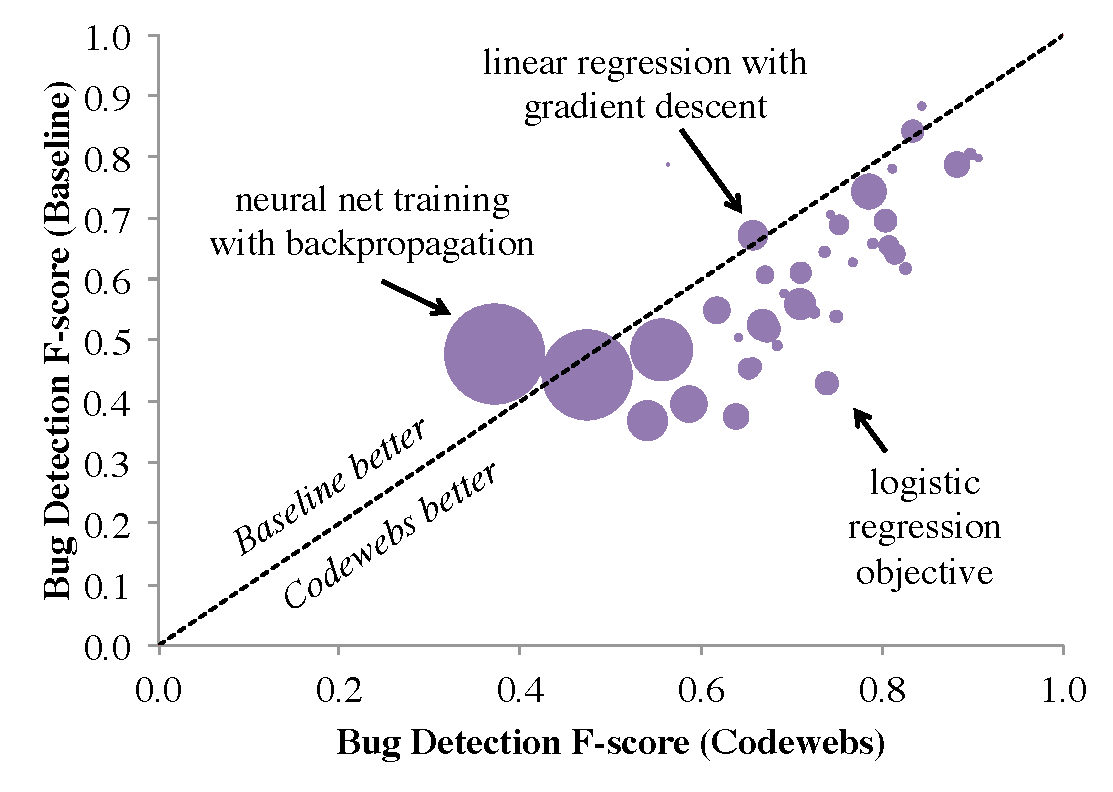
\includegraphics[width=.31\textwidth]{img/bugsFscoreDiffs.pdf}
\label{fig:bugsAll}

}
\qquad\qquad
\subfigure[]{
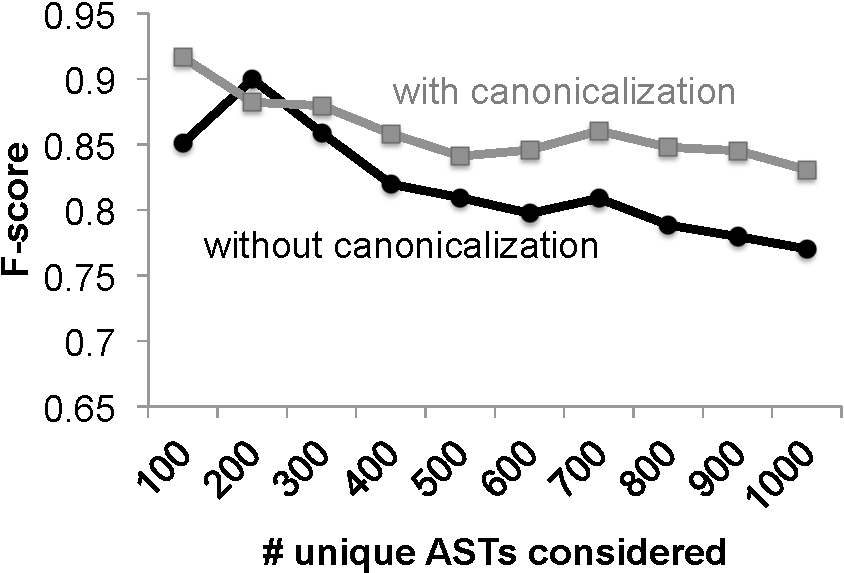
\includegraphics[width=.3\textwidth]{img/bugIsolation.pdf}
\label{fig:bugIsolation}
}

\caption[Bug detection accuracy]{
\subref{fig:bugsAll}  F-score comparison of Codewebs based bug detection algorithm against baseline (5-nearest neighbors) 
for the 5000 most frequent ASTs for each assigned homework problem.  Each circle corresponds to a single homework problem, 
with circle widths  set to be proportional to the average \# of nodes per AST for that problem; 
\subref{fig:bugIsolation} Codewebs based bug detection F-scores on the $k$ most frequent ASTs, with and without canonicalization
on the ``linear regression with gradient descent'' homework problem.
}
\label{fig:exp2}
\end{figure}


Considering buggy programs as positive examples, we evaluate the precision and recall
of both classifiers on the 5000 most frequent ASTs for each homework problem in the class
and compute the \emph{F-score} (i.e., the harmonic mean of precision and recall, with higher values
corresponding to higher accuracy) in each case.
Figure~\ref{fig:bugsAll} compares this F-score performance of our query based bug detection
algorithm against that of $k$NN.   As a rough measure of problem complexity, we also visualize
 the average number of nodes per AST in each problem (after subtracting
the number of AST nodes that come from the provided starter code) by varying circle sizes.
As can be seen in the plot, bug detection is generally more difficult for both approaches on the more
complex assignments, with the neural network training problems being the most difficult.
%Points below the diagonal in this plot correspond to homework problems
%on which our Codewebs based bug detector outperforms the baseline algorithm.
However in many problems, we obtain reasonable accuracy using both approaches with
the Codewebs based algorithm outperforming the baseline in most cases.

%Our algorithm is successful with most points lying in the upper right corner of the scatter plot.
%The two problems on which our algorithm had the most difficulty were related to the neural network backpropagation assignment,
%in which the submitted implementations were significantly lengthier than those of other problems (with over 40 lines of code per implementation).

%To show that our algorithm performs the best for the most frequently submitted ASTs,
Figure~\ref{fig:bugIsolation} plots the performance  of our detection algorithm
on the 100 most frequent ASTs, 200 most frequent, and so on for the linear regression problem.
As in our reduction experiments, performance is better 
for the more frequently submitted ASTs, and the drop in accuracy as we get to less frequent ASTs is graceful.
Using canonicalization again helps to boost performance in general.
On 1000 ASTs, our bug detection precision (with canonicalization) is .78 and recall is .88.
Finally, we remark that the bug localization algorithm is fast and capable of  handling over 150 requests per second (for the
linear regression problem with an average AST size 116).

\mypara{Feedback case study}
Without the help of our system, the easiest way to scalably provide feedback to students in a MOOC is to 
send canned feedback for the most frequent (incorrect) unit test outcomes, which often reflect common misunderstandings.
One weakness of this unit-test based approach, however, is that it can fail when a single conceptual misunderstanding
can lead to multiple unit test outcomes, or when it occurs in the presence of other bugs.
We  illustrate  how the Codewebs system can be used to give feedback to students even
when the unit-test based approach fails.

In the linear regression problem, many students
erroneously included an ``extraneous sum'' in the gradient expression
(e.g., with $\texttt{sum((X*theta-y)'*X)}$ instead of   $\texttt{X'*(X*theta-y)}$ ). 
Upon identifying a single instance of the bug, an instructor can then use
the Codewebs system 
to extract many equivalent ways of writing the erroneous expression (e.g., $\texttt{sum(((theta'*X')'-y)'*X)}$, $\texttt{sum(transpose(X*theta-y)*X)}$, etc.).   
These expressions are then matched to incoming student submissions, for which we can
provide a human generated message explaining the cause of the misunderstanding.

After extracting equivalences and matching to the existing submissions, our algorithm
found 1208 submissions which matched the ``extraneous sum'' bug, outperforming a unit test based
feedback strategy which would have covered 1091 submissions.  We can also use both strategies together, giving feedback to submissions found by either
method to contain the bug, 
which would lead to a 47\% increase in number of submissions covered over just using unit tests.

\section{Related work}\label{sec:relatedwork}
Our paper builds upon a body of work on reasoning with code collections --- a problem that arises
both for programmers and for those learning to program.  
Code search engines, many of which scale to massive databases 
have been proposed, for example, for the purposes of code reuse or navigating a complicated API~\cite{sindhgatta06,hoffmann07}.
A number of choices exist in this domain of reasoning with a code collection.
How much structure to take into account is one such choice, 
with some systems reasoning at the level of keywords or tokens~\cite{hummel08, hartmann10} to other systems reasoning
with the full syntactic 
structure of the AST~\cite{paul94, thummalapenta07,kim10}.
Canonicalization has been a popular approach for reducing the variance of a large collection of code  in many such works~\cite{baxter98,xu03}.
In contrast to our paper, this work on code search engines generally has focused on helping programmers to understanding what tools in an existing 
codebase can help a programmer to accomplish 
a certain task, which is reflected by features that are commonly supported, such as the ability to query for usage examples for a function, 
or to find methods that require a certain type as a parameter.  
Closer to our setting is the work of Rivers et al.~\cite{rivers12,rivers13}, who also used ASTs with canonicalization to map out the solution space to 
introductory programming problems and discover common errors.

However, reasoning about function is critical in many settings, and thus
another choice that has received recent attention is whether to incorporate 
unit test information~\cite{hummel08,lazzarini09}.  
Our work efficiently combines what we believe to be the best of the above ideas: reasoning with ASTs and unit tests, as well as combining the
two sources of data to automatically discover semantically equivalent code phrases.  To our knowledge, this is
the first method for automatically finding canonicalization rules for programs.

%Reasoning with a collection of code for educational purposes is a more recent topic which we
%predict will become more prevalent in the literature as MOOC datasets become more widely available 
%to researchers.

The idea that student code can be ``clustered'' into a small category of approaches has also been explored by a number of researchers.
Piech et al.~\cite{piech12}, for example, cluster trajectories of ASTs over multiple submits by a single student.  
Glassman et al.~\cite{glassman13} visualize the space of student solutions to Matlab programming problems in order to identify popular approaches for
solving a problem.
A number of recent papers have clustered students based on abstract syntax trees using distances in feature 
space~\cite{gross12,gross13}, string edit distance~\cite{rivers12,rivers13}
and tree edit distance~\cite{huang13}, proposing to give feedback to exemplar submissions.	
These methods rely almost completely on syntactic analysis and do not 
explicitly relate form to function as in our work. Furthermore, for assignments with multiple ``parts'', each of which can be approached in multiple ways, 
the number of clusters intuitively can grow exponentially in the number of parts, leading to a loss of interpretability and effectiveness of the method.
Our work is the first to explicitly address the idea that smaller parts of code can be shared among submissions.

\section{Discussion}\label{sec:discussion}
MOOC platforms now collect massive datasets of student submissions across hundreds of courses, 
introducing new research problems of how to organize and search the data 
effectively, but also new opportunities to use the data in ways that were not previously possible.
We have developed a system called Codewebs which efficiently indexes all of the code submissions to a 
MOOC programming assignment and can be useful in a number of applications.  
Through a novel use of unit test information, our system is also able to determine 
when code snippets are semantically equivalent in a data driven way.

As the MOOC ecosystem continues to quickly expand, it is crucial for 
accompanying learning technologies to be applicable to a large variety of courses with minimal effort on the part of the instructor.
Codewebs makes no assumptions about the underlying assignments and is designed to be easily applicable to a 
wide variety of programming languages.
Instead of running dynamic analysis on fully instrumented programs, the system relies only on unit test information
which is lightweight and thus contributes to portability.
To apply Codewebs to a programming problem, the most important requirement is a large dataset of student submissions (which is a given in MOOCs).
Beyond data, we only have a handful of requirements:
(1) a mechanism for parsing source code into an abstract syntax tree (which is available for most programming languages)
(2) a specification of which nodes of an AST correspond to statements, identifiers, and constants, 
(3) a listing of reserved functions and identifiers that are not to be anonymized, 
(4) sufficiently informative unit tests for problems, and 
(5) instructor specified
points of variation for determining canonicalization rules.  
Thus we believe that applying the Codewebs system to submissions in other coding intensive courses should be straightforward.

There are a number of directions ripe for future work.
At the moment, our system only handles code that parses correctly.  However for beginning programmers,
even writing syntactically valid code can be a challenge.  Thus the question of how to leverage a large
dataset for giving feedback to unparseable submissions remains an important open problem.  
Our current approach is also limited to indexing submissions of a single function where all implementations receive
the same input and thus can be unit tested in a unified way.
Thus another open problem is how to deal with long form programs in which
students are free to choose how to decompose an implementation into smaller modules.

We believe  many of the insights that went into creating the Codewebs system
may also apply to general search engines for source code outside of the educational setting. 
But more interestingly, these ideas may also apply to indexing formal logic proofs~\cite{fast13} and equations~\cite{kohlhase06}, or even 
natural language mathematical proofs, which can be useful either for researchers or educators.
%or in math and statistics courses offered online.
Looking even further, it is tantalizing to speculate about the role that effective search engines for student content
 might play in the MOOC ecosystem beyond STEM (science, technology, engineering and mathematics) courses. 
Public exhibitions of student work are, for example, a common way to culminate university level art and design courses --- but 
pulling these exhibitions off at the scale of MOOCs requires an effective way to search through tens of thousands of submissions.
And while the specific features of designing a search engine for one of these courses will surely be different from the Codewebs
setting,  many of the same questions will still apply.  
What are the natural queries for an assignment?
How can we exploit the organizational structure of a search engine index to facilitate student feedback?
How do we scale to tens of thousands of students?

\subsection*{Acknowledgments}

We thank Andrew Ng, Daphne Koller, John Mitchell, and Mehran Sahami for 
useful conversations.
%J. Huang is supported by an NSF Computing Innovations Fellowship 
%and C. Piech is supported by an NSF Graduate Fellowship.
This research was funded by
NSF grants CCF 1011228 and  DMS 1228304, AFOSR grant FA9550-12-1-0372,  a Google Research Award, and the Max Planck Center for Visual Computing and Communications.
J. Huang is supported by the CRA CI Fellows grant 104672, and C. Piech by the NSF

\chapter{Homework Embedding Spaces}
\begin{figure}[h!]
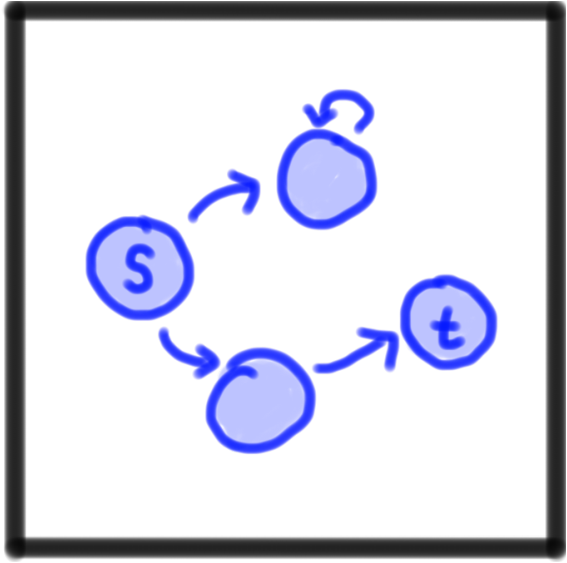
\includegraphics[width=0.2\textwidth]{img/assnType_3}
\end{figure}

In elementary programming tasks that are used by millions of students we can use emergent patterns in how students navigate the space of solutions to autonomously generate hints. However this strategy relies on having a relatively dense coverage of the partial solutions. When we look at the next level of assignment richness, the space of intermediate solutions students produced is too sparse for the Problem Solving Policy approach. 

In this chapter we develop approaches for giving feedback to students for control flow assignments that are typical as the first assignments in university courses. In these tasks, students write programs using a language that is often turing complete and has all the control flow affordances of modern programming languages, but no user defined variables. Feedback in this domain often is in the form of human comments to the whole (or parts) of a partial solution. 

A central difficulty that arises as we look at this set of programs is that even though as humans we can see structure and patterns in student submissions, it is difficult for computers to find structure in data in the form of programs.  Program representations
such as the Abstract Syntax Trees are not directly conducive to standard statistical methods and the edit distance metric between such trees 
are not discriminative enough to be used to share feedback accurately since programs with similar ASTs can behave quite differently and require different comments. 

There are two major goals of this chapter.  The 
first is to automatically learn a feature embedding of 
student submitted programs
that captures functional and stylistic elements and can be easily
used in typical supervised machine learning systems.
The second is to use these features to learn
how to give automatic feedback to students. Inspired by recent successes of deep learning for learning features 
in other domains like NLP and vision, 
we formulate a novel neural network architecture 
that allows us to jointly optimize an embedding of programs and memory-state in a feature space.
%We propose the use of neural networks to jointly learn an embedding of states and programs that best captures these pre-condition, program, post-condition triples. 
See Figure~\ref{fig:splash} for an example program and corresponding matrix embeddings.


%A unique property of programs is that they are 
To gather data, we exploit the fact that programs are 
executable --- that we can evaluate any piece of code on 
an arbitrary input (i.e., the precondition), and observe the state  
after, (the postcondition). For a program and its 
constituent parts we can thus collect arbitrarily many such precondition/postcondition mappings. This %deluge of data 
data provides the training set from which we can learn a shared representation for programs. 
To evaluate our program embeddings we test our ability to amplify teacher feedback. We use real student data from the Code.org Hour of Code which has been attempted by over 27 million learners
%and has been taught in over 90 thousand classrooms, 
making it, to the best of our knowledge,
the largest online course to-date. 
We then show how the same approach can be used for submissions in Stanford University's Programming Methodologies course which has thousands of students and assignments that are substantially more complex. The programs we analyze are written in a Turing-complete language but do not allow for user-defined variables.

Our main contributions are as follows. First, we present a 
method for computing features of code that capture both functional
and stylistic elements.  Our model works by simultaneously embedding precondition and postcondition spaces of 
a set of programs into a feature space where programs can be viewed as linear maps on this space.
Second, we show how our code features can be useful for automatically
propagating instructor feedback to students in a massive course.
Finally, we demonstrate the effectiveness of our methods
on large scale datasets.
%model 
%which allows us to simultaneously embed input and output spaces of 
%a collection of programs into a Euclidean space where programs can be viewed as linear map on this space. Second, we demonstrate the effectiveness of this model applied to two tasks: that of predicting the results of running a program on a given precondition and of propagating teacher feedback to a large number of students. 
%Finally, we explore the relationship between program complexity and the performance of machine learning tasks using our program embeddings.
Learning embeddings of programs is fertile ground for machine learning research and if such embeddings can be useful for the propagation of teacher feedback this line of investigation will have a sizable impact on the future of computer science education.

\begin{figure}[t]
\centering
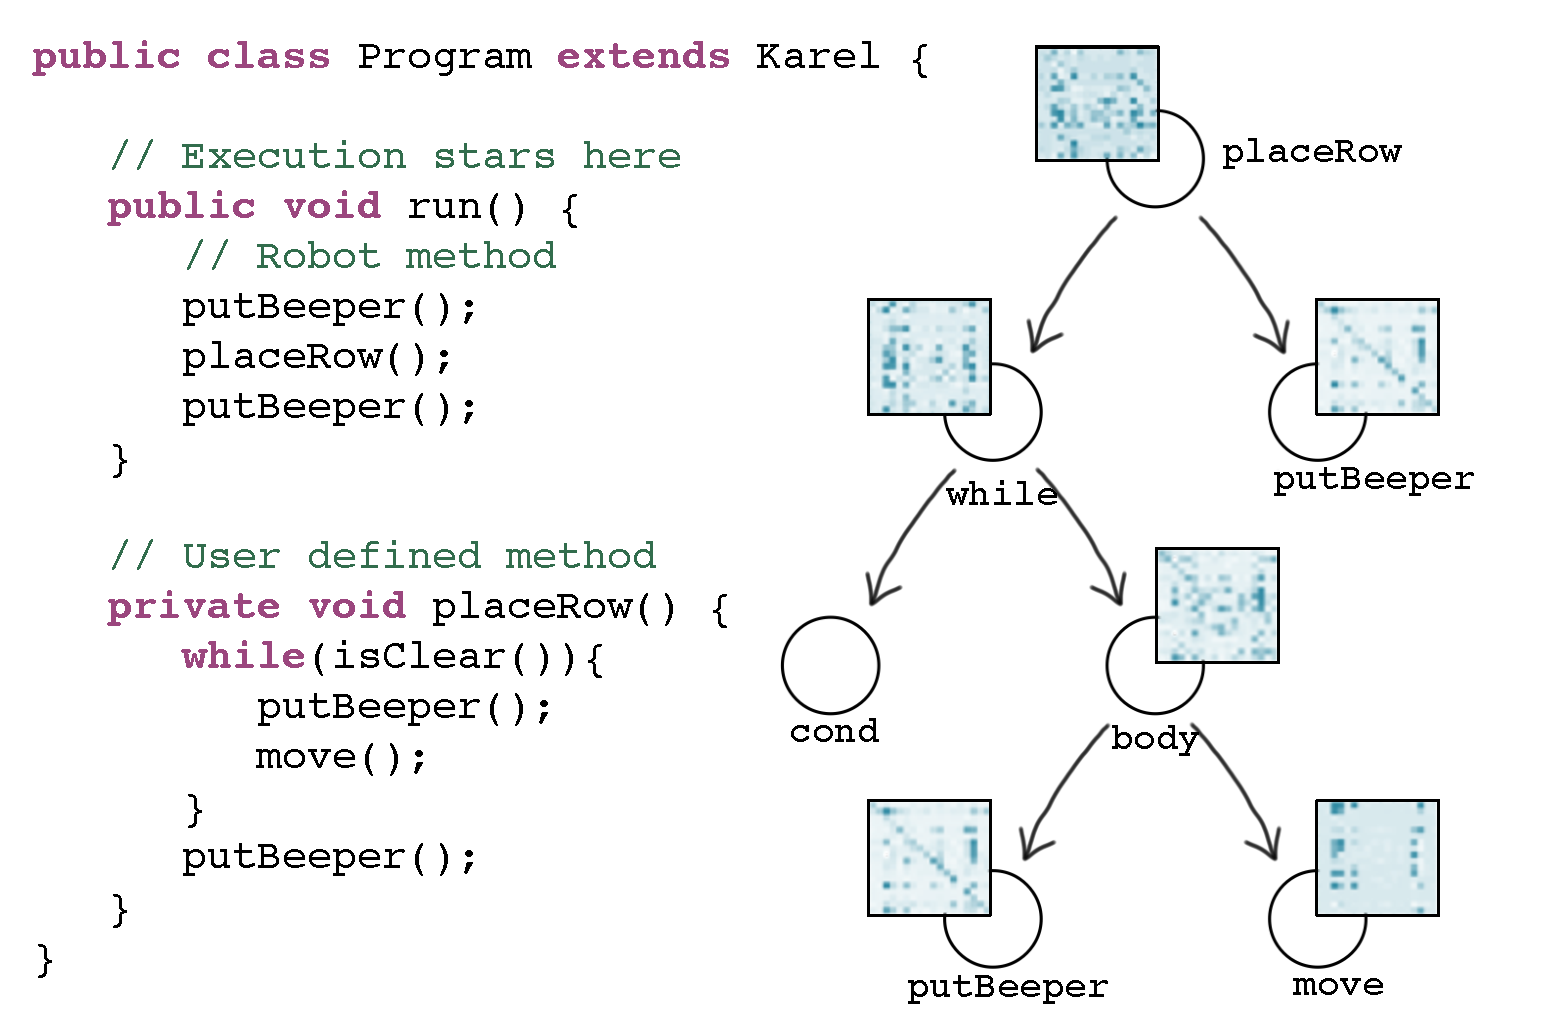
\includegraphics[width=.65\columnwidth]{img/splash2_noborder}
\caption{We learn matrices which capture functionality. Left: a student partial solution. Right: learned matrices for the syntax trees rooted at each node of placeRow.}
\label{fig:splash}
\end{figure}

\section{Related Work}\label{sec:related}
The advent of massive online computer science courses 
has made the problem of automated reasoning with large code
collections an important problem.
There have been a number of recent papers~\cite{huangetal13,basu2013powergrading,nguyen14,brooks2014divide,lan2015mathematical, piech2015} on using large
homework submission datasets to improve student feedback. The volume of work speaks to the importance of this problem. Despite the research efforts, however, providing quality feedback at scale remains an open problem. 

A central challenge that a number of papers
 address is that of measuring similarity between 
source code.
Some authors have done this without an explicit 
featurization of the code ---
for example, the \emph{AST edit distance} has been a popular choice~\cite{huangetal13,rogers2014aces}.
\cite{mokbel2013domain} explicitly 
hand engineered a small collection of features on ASTs
that are meant to be domain-independent. 

To incorporate functionality,
\cite{nguyen14} proposed a method that discovers program modifications that do not appear to change the semantic meaning of code. 
The embedded representations of programs used in this paper also capture semantic similarities and are more amenable to prediction tasks such as propagating feedback. 
We ran feedback propagation on student data using methods from Nguyen et al and observe that embeddings enabled notable improvement (see section 6.3).
%While this approach was useful,
%determining absolute equivalence is an unsolvable problem and it quickly becomes hard to decide when we have enough evidence to label code as being the same. The methods in this paper allow for different degrees of similarity and a more direct means to use program similarities to propagate feedback. %it is not fully automated, which makes its application to new problems difficult, and is unable to 
%and while it helps reduce the complexity of a corpus of student programs the extent to which it can be used to propagate functional feedback is constrained by the large combinatorial number of student solutions and such a method is unable to 
%disseminate stylistic comments.
%Our method, by contrast, allows for more general propagation of comments and can be inserted into other machine learning systems.

Embedding programs has many crossovers with embedding natural language artifacts, given the similarity between the AST representation and parse trees. Our models are related to recent work from the NLP and deep learning communities on recursive neural networks, particularly
for modeling semantics in sentences or symbolic expressions~\cite{socher2013recursive,socher2011semi,zaremba2014learningb,bowman2013can}.
%illustrate the effectiveness of Recursive Neural Networks (RNNs) and Recursive Neural Tensor Networks. 

Finally, representing a potentially 
complicated function (which in our case is a program) as
a linear operator acting on a nonlinear feature space has also
been explored in different communities.
The computer graphics community
have represented pairings of nonlinear geometric
shapes as linear maps between shape features, called \emph{functional maps}~\cite{ovsjanikov2012functional,ovsjanikov2013analysis}.
From the kernel methods literature, there has also been recent
work on representations of conditional probability
 distributions as operators on a Hilbert space~\cite{song2013kernel,song2009hilbert}. 
From this point of view, our work is novel in that it
focuses on the joint optimization of feature embeddings
together with a collection of maps
so that the maps simultaneously ``look linear''
with respect to the feature space.



\section{Embedding Hoare Triples}\label{sec:embedding}

\begin{figure*}[t]
\centering
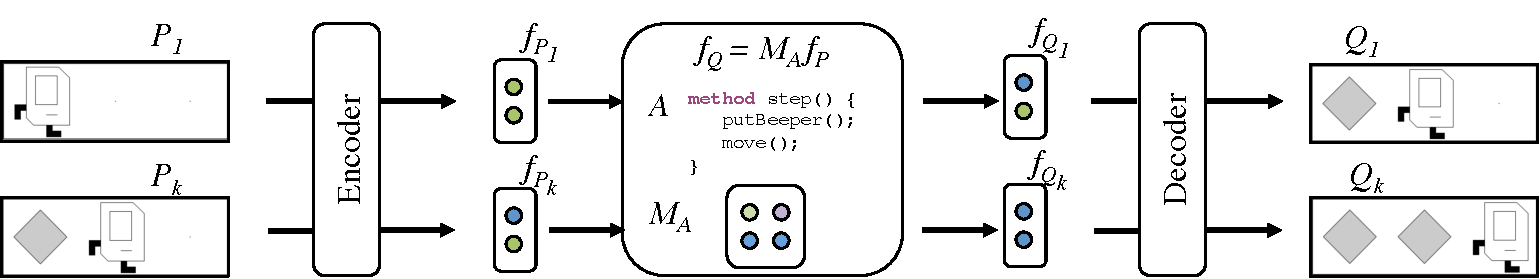
\includegraphics[width=1.0\textwidth]{img/overview}
\caption{
Diagram of the model for a program $A$ implementing a simple ``step forward'' behavior
in a small 1-dimensional gridworld. Two of the $k$ Hoare triples that correspond with $A$ are shown. Typical worlds are larger and programs are more complex.
}
\label{fig:hoare}

\end{figure*}
Our core problem is to represent a program as a point in a fixed-dimension real-valued space that can then be used directly as input for typical supervised learning algorithms.

While there are many dimensions that ``characterize'' a program including
aspects such as style or time/space complexity, we begin by 
first focussing on capturing the most basic aspect of a program --- its function.  While capturing the function of the program ignores
aspects that can be useful in application (such as giving
stylistic feedback in CS education), we discuss in later
sections how elements of style can be recaptured by modeling the
function of subprograms that correspond to each subtree of an AST.
Given a program $A$ (where we consider a program to generally be any executable code whether a full submission or a subtree of a submission), and a precondition $P$, we thus would
like to learn features of $A$ that are useful for predicting the outcome of running $A$ when $P$ holds.  In other words, we want to 
predict a postcondition $Q$ out of some space of possible postconditions. Without loss of generality we let $P$ and $Q$ be 
real-valued vectors encapsulating the ``state'' of the program (i.e., the values of all program variables)
at a particular time. For example, in a grid world, this vector would contain the location of the agent, the direction the agent is facing, the status of the board and whether the program has crashed. Figure \ref{fig:hoare} visualizes two preconditions, and the corresponding postconditions for a simple program. 

We propose to learn program features using a training set of $(P, A, Q)$-triples --- so-called \emph{Hoare triples}~\cite{hoare1969axiomatic}
obtained via historical runs of a collection of programs on a collection of preconditions.
%The dimensions
%of $P$ and $Q$ are assumed to be fixed across all instances in a training set.
We discuss the process by which such a dataset can be obtained  in Section~\ref{sec:data}. 
The main approach that we espouse in this paper is to simultaneously find an embedding of states and programs into feature space where pre and postconditions are points in this space and programs are mappings between them.

The simple way that we propose to relate preconditions to postconditions
is through a linear transformation.  Explicitly, given a
$(P, A, Q)$-triple, if $f_P$ and $f_Q$ are $m$-dimensional nonlinear feature
representations of the pre and postconditions $P$ and $Q$, respectively,
then we relate the embeddings via the equation
\begin{equation}\label{eqn:linearmap}
f_Q = M_A \cdot f_P.   
\end{equation}
We then take the $m\times m$ matrix of coefficients $M_A$
as our feature representation of the program $A$ and refer to it as
the \emph{program embedding matrix}. 
We will want to learn the mapping into feature space $f$ 
as well as the linear map $M_A$ such that 
this equality holds for all observed triples and can
generalize to predict postcondition $Q$ given $P$ and $A$.


At first blush, this linear relationship may seem too limiting
as programs are not linear nor continuous in general.  By learning a nonlinear embedding function $f$ for the pre and postcondition spaces,
however, we can capture a rich family of nonlinear relationships
much in the same way that kernel methods allow for nonlinear decision boundaries.

As described so far, there remain a number of modeling choices to be made. In the following, we elaborate further on how we model the
feature embeddings $f_P$, and $f_Q$ of the pre and postconditions, and how to model the program embedding matrix $M_A$.


\subsection{Neural network encoding and decoding of states}
We assume that preconditions have some base encoding as a $d$-dimensional vector, which we refer to as $P$.
For example, in image processing courses, the state space could simply be
the pixel encoding of an image, whereas
in the discrete gridworld-type programming problems that we use in our experiments, we might choose to encode the $(x,y)$-coordinate
and discretized heading of a robot using a concatenation of 
one-hot encodings. 
Similarly, we assume that there is a base encoding $Q$ of the postcondition.

We will focus our exposition in the remainder of our paper
on the case where the precondition space 
and postcondition spaces share a common base encoding.  This is particularly
appropriate to our experimental setting in which both the preconditions
and postconditions are representations of a gridworld.  In this case, we can use the same decoder parameters 
(i.e., $W^{dec}$ and $b^{dec}$) to decode both from precondition space and postcondition space
 --- a fact that we will exploit in the following section.  


Inspired by nonlinear autoencoders, we parameterize a mapping, called
the \emph{encoder} from 
precondition $P$ to a nonlinear $m$-dimensional
feature representation $f_P$.
As with traditional autoencoders, we use an affine mapping composed
with an elementwise nonlinearity:  
%Using $\tanh$ nonlinearities (as is done
%in our experiments), we would thus have:
\begin{equation}\label{eqn:encodeprecondition}
f_P =  \phi(W^{enc}\cdot P + b^{enc}),
\end{equation}
where $W^{enc}\in\reals^{m\times d}$, $b^{enc}\in \reals^m$,
and $\phi$ is an elementwise nonlinear function (such as $\tanh$).
At this point, we can use the representation
$f_P$ to decode or reconstruct the original precondition as 
a traditional autoencoder would do using:
\begin{equation}\label{eqn:decodeprecondition}
\hat{P} =  \psi (W^{dec}\cdot f_P + b^{dec}),
\end{equation}
where $W^{dec}\in\reals^{d\times m}$, $b^{dec}\in\reals^{d}$,
and $\psi$ is some (potentially different) elementwise 
nonlinear function.
Moreover, we can push the precondition
embedding $f_P$ through Equation~\ref{eqn:linearmap}, and decode the
postcondition embedding $f_Q=M_A\cdot f_P$.  This mapping which reconstructs
the postcondition $Q$, the \emph{decoder}, takes the form:

{
\begin{align}
\hat{Q} &= \psi (W^{dec}\cdot f_Q + b^{dec}), \label{eqn:decodepostcondition}\\
    &= \psi (W^{dec}\cdot M_A\cdot f_P + b^{dec}).
\end{align}
}

%Rather than being interpreted as a strict reconstruction of $Q$,
%the softmax function allows us to interpret $\hat{Q}$ as a probability
%distribution over the space of possible postconditions.
Figure~\ref{fig:hoare} diagrams our model on a simple program.
Note that it is possible to swap in alternative feature representations.
We have experimented with using a deep, stacked autoencoder however our results have
not shown these to help much in the context of our datasets.

\subsection{Nonparametric model of program embedding}\label{sec:nonparametric}
%Thus far, we have discussed encoder and decoder parameters for our model.
%What remains is a model for the program embedding matrix. 
To encode the program embedding matrix, we propose a simple
nonparametric model in which each program in the training set is associated
with its own embedding matrix.
Specifically, if the collection of unique programs
is $\{A_1,\dots,A_m\}$, then for each $A_i$, we will associate a matrix $M_i$.
The entire parameter set for our nonparametric
matrix model (henceforth abbreviated \emph{NPM}) is thus:
$\Theta=\{W^{dec}, W^{enc}, b^{enc}, b^{dec}\}\cup\{M_i\,:\,i=1,\dots,m\}$.

To learn the parameters, we minimize a sum of three terms: (1) a prediction loss
$\ell^{pred}$ which quantifies how well we can predict postcondition of a program 
given a precondition, (2) an autoencoding loss $\ell^{auto}$ which quantifies how good 
the encoder and decoder parameters are for reconstructing given preconditions, and (3) a regularization term $\mathcal{R}$.
Formally, given training triples $\{(P_i, A_i, Q_i)\}_{i=1}^n$,
we can minimize the following objective function:

{
\begin{align}
\begin{split}
L(\Theta) &=  \frac{1}{n} \sum_{i=1}^n 
                \ell^{pred}(Q_i, \hat{Q}_i(P_i, A_i; \Theta)) \\
        %\ell^{pred}(\Theta; Q_i, \hat{Q}_i, Pi, A_i)   \\
    &\;\;+  \frac{1}{n} \sum_{i=1}^n 
                    \ell^{auto}(P_i, \hat{P}_i(P_i, \Theta)) 
        %    \ell^{auto}(\Theta; Q_i, \hat{Q}_i, Pi, A_i) 
    + \frac{\lambda}{2}\mathcal{R}(\Theta), \label{eqn:objective}
  \end{split}
\end{align}
}

where
$\mathcal{R}$ is a regularization term on the parameters,
and $\lambda$ a regularization parameter.
In our experiments, we use $\mathcal{R}$ to penalize the sum of the $L_2$ norms of the
weight matrices (excluding the bias terms $b^{enc}$ and $b^{dec}$).

Any differentiable loss can conceptually be used for $\ell^{pred}$ and
$\ell^{auto}$.  For example,
when the top level predictions, $\hat{P}$ or $\hat{Q}$,
can be interpreted as probabilities (e.g., when $\phi$ is
the Softmax function), we use a cross-entropy loss function.



Informally speaking, one can think of our optimization problem (Equation~\ref{eqn:objective}) as trying to
find a good \emph{shared} representation of the state space ---
shared in the sense that 
even though programs are clearly not linear maps over the
original state space, the hope is that we can discover some 
nonlinear encoding of the pre and postconditions such that most
programs simultaneously 
``look'' linear in this new projected feature space.
As we empirically show in Section~\ref{sec:experiments}, such a representation
is indeed discoverable.

We run joint optimization using minibatch stochastic gradient 
descent without momentum, 
using ordinary backpropagation to calculate the gradient.
We use random search~\cite{bergstra2012random}
to optimize over hyperparameters (e.g, regularization parameters,
matrix dimensions, and minibatch size).
Learning rates are set using Adagrad~\cite{duchi2011adaptive}. We seed our parameters using a ``smart'' initialization 
in which we first learn an
autoencoder on the state space, and perform a vector-valued ridge
regression for each unique program
to extract a matrix mapping the features of the precondition
to the features of the postcondition.  The encoder and decoder parameters and the program matrices are then jointly optimized.


%\Jon{We initialize gradient descent
%by randomizing all parameters.  Does this belong here or at the top of %the paragraph?
%And just for parametric model.}

%The idea here is that we would like to learn a representation of the %pre and post conditions
%that's good for representing multiple programs
% simultaneously as linear maps.
% We can discuss how for a neural network autoencoder
% this is always possible (in terms of representational
% power) for a single program.
%I.E. We are finding shared structure amongst states
%and shared structure amongst the transformations.


%Thusly formulated, our model bears some resemblance to traditional
%autoencoders, particularly when the precondition and postcondition
%spaces are the same.


%Introduce the general idea of embedding a program
%as a fixed size representation.
%Need to account for inputs to capture
%functionality, so propose matrix representation.
%
%Introduce our model: Hoare triple embedding. Capture all Huare triples for a given piece of code.
%Explain encoder, decoder.  Discuss loss functions ---
%emphasize the point that we are training the 
%representation of the pre/post conditions with the
%representation of the transformation.

%Discuss the fact that when precondition space and
%postcondition space are the same (which is sometimes
%the case in educational programs), we can enforce loss
%at two points




%#Explain training.  Initialization via auto-encoders for states and %ridge
%regression.  Followed by joint training.
%We can say that we used adagrad.
%Our first goal is to learn an embedding which can capture the %functionality of any program or sub-program.


\subsection{Triple Extraction}\label{sec:triplets}
For a given program $S$ we extract Hoare triples by executing it on an exemplar set of unit tests. These tests span a variety of reasonable starting conditions. We instrument the execution of the program such that each time a subtree $A \subset S$ is executed, we record the value, $P$, of all variables before execution, and the value, $Q$, of all variables after execution and save the triple ($P$, $A$, $Q$). We run all programs on unit tests, collecting triples for \emph{all} subtrees. Doing so results in a large dataset $\{(P_i, A_i, Q_i)\}_{i=1}^n$ from which we collapse equivalent
triples.
In practice, some subtrees, especially the body of loops, generate a large (potentially infinite) number of triples. To prevent any subtree from having undue influence on our model we limit the number of triples for any subtree. 

Collecting triples on subtrees, as opposed to just collecting triples on complete programs, is critical since it allows us to learn embeddings not just for the root of a program AST but also for the constituent parts. As a result, we retain data on how a program was implemented, and not just on its overall functionality, which is important for student feedback as we discuss in the next section.
Collecting triples on subtrees also means we are able to optimize our embeddings with substantially more data.
%crucial for both the parametric and non-parametric program embeddings. In the non-parametric setting collecting subtree triples allows us to learn embeddings not just for the root of a program AST but also for the constituent parts.  For the parametric model, collecting triples on subtrees means we are able to train our embeddings with substantially more data. This is especially important as it provides training examples for nodes deeper ASTs with weights that are otherwise hard to learn by recursively back-propagated gradients.
%We share triples across identical subtrees.

\section{Feedback Propagation}\label{sec:feedback}
The result of jointly learning to embed states and 
a corpus of programs is a fixed dimensional, real-valued matrix $M_A$ for each subtree $A$ of any program in our corpus. These matrices can be cooperative with machine learning algorithms that can perform tasks beyond predicting what a program does. 
The central application in this paper is the force multiplication of teacher-provided feedback where an active learning algorithm interacts with human graders such that feedback is given to many more assignments than the grader annotates. We propose a two phase interaction. In the first phase, the algorithm selects a subset of exemplar programs for graders to apply a finite set of annotations. Then in the second phase, the algorithm uses the human provided annotations as supervised labels with which it can learn to predict feedback for unlabelled submissions. Each program is annotated with a set $H \subset L$ where $L$ is a discrete collection of $N$ possible annotations. The annotations are meant to cover a range of comments a grader could apply, including feedback on style, strategy and functionality. For each ungraded submission, we must then decide which of the $N$ labels to apply. As such, we view feedback propagation as $N$ binary classification tasks. 

%Ideally, feedback for programs in an educational setting would comment on both functionality and style. Students are learning not just how to write programs that solve tasks, but how to do so in an artful way. 
One way of propagating feedback would be to use the elements of the embedding matrix of the root of a program as features and then train a classifier to predict appropriate feedback for a given program.  However, the matrices we have learned for programs and their subtrees have been trained only to predict functionality.  Consequently, any two programs that are functionally indistinguishable would be given the same instructor feedback under this approach, ignoring any strategic or stylistic differences between the programs.
%This is problematic in the case where the model becomes too capable, %and are able to represent nodes just based on what they do and not the %way in which the code-phrase was implemented. This is clearly the case for the non-parametric program matrix model. 
%Only representing what a program does means that feedback pertaining to style or strategy cannot be predicted.


\subsection{Incorporating structure via
    recursive embedding}
To recapture the elements of program structure and style 
that are critical for student feedback, our approach to predict feedback uses
the embedding matrices learned for the NPM model, but incorporates
all constituent subtrees of a given AST.
%One could imagine multiple ways of predicting feedback given an abstract syntax tree where each node has a corresponding matrix representation of its observed hoare-triples. We propose that to propagate feedback we learn a model which recursively feeds-forward annotation information up the AST incorporating $M_l$ at each node $l$.
Specifically, using the embedding matrices learned in the NPM model
(which we henceforth denote as $M^{NPM}_A$ for a subtree $A$),
we now propose a new model
based on recursive neural networks (called the \emph{NPM-RNN} model)
in which
we parametrize a matrix $M_A$ in this new model
with an RNN whose
architecture follows the abstract syntax tree 
(similar to the way in which RNN architectures might take the form of a parse tree in an NLP 
setting~\cite{socher2013recursive}).

In our RNN based model, % which we denote the \emph{NPM-RNN model}, 
a subtree of the 
AST rooted at node $j$ is represented
by a matrix which is computed by combining (1) representations of subtrees rooted
at the children of $j$, and (2) the embedding matrix of the subtree
rooted at node $j$ learned via the NPM model.
By incorporating the embedding matrix from the NPM model, we are able to capture the function of every subtree in the AST.

Formally, we will assume each node is associated with some \emph{type}
in set $\mathcal{T}=\{\omega^1, \omega^2,\dots\}$.  Concretely, the type set might
be the collection of keywords or built-in functions that can be called from a program 
in the dataset, e.g., $\mathcal{T}=\{\mathbf{repeat}, \mathbf{while}, \mathbf{if}, \dots\}$.
A node with type $\omega$ is assumed to have a fixed number, $a_\omega$, of children in the AST --- 
for example, a $\mathbf{repeat}$ node has two children, with one child holding the body
of a repeat loop and the second representing the number of times the body is
to be repeated.   

The representation of node $j$ with type $\omega$ 
is then recursively computed in the NPM-RNN model via:

{
\begin{equation}\label{eqn:feedbackRnn}
a^{(j)} = \phi\left( \sum_{i=1}^{a_\omega} W_i^\omega \cdot a^{(c_i[j])} + b^\omega + \mu M^{NPM}_j \right),
\end{equation}
}

where: $\phi$ is a nonlinearity (such as $\tanh$), $c_i[j]$ indexes over
the $a_\omega$ children of node $j$, and $M^{NPM}_j$ is the program embedding matrix learned in the NPM model for the subtree rooted at node $j$.  We remind the reader that the activation $a^{(j)}$ at
each node is an $m\times m$ matrix.
Leaf nodes of type $\omega$
are simply associated with a single parameter matrix
$W^\omega$.


In the NPM-RNN model,
we have parameter matrices $W^\omega, b^\omega \in \reals^{m\times m}$ for each possible type 
$\omega \in \mathcal{T}$.
To train the parameters, we
first use the NPM model to compute the 
embedding matrix $M^{NPM}_j$ for each subtree. 
After fixing $M_j$,  we optimize (as with the NPM model)
with minibatch stochastic
gradient descent using backpropagation through structure~\cite{goller1996learning} to compute gradients.
Instead of optimizing for predicting postcondition,
for NPM-RNN, we optimize for each of the binary prediction tasks
that are used for feedback propagation given the vector embedding
at the root of a program. We used hyper-parameters learned in the RNN model optimization since feedback optimization is performed over few examples and without a holdout set.

%Feedback is then predicted using logistic regression off of the %activation of the root, and back-propagated. The parametric model is %already a RNN as such we can simply update the existing parameters.

%\subsection{Active learning}

Finally, feedback propagation has a natural active learning component: 
intelligently selecting submissions for human annotation 
can potentially save instructors significant time.
We find that in practice, running $k$-means on the learned embeddings,
and selecting the cluster centroids as the set of submissions to be annotated works well and leads to significant improvements in feedback propagation
over random subset selection. Surprisingly, having humans annotate the most common programs performs worse than the alternatives, which we
observe to be due to the fact that the most common submissions are all quite similar to one another.

%We experiment with selecting the most popular submissions, randomly %sampled programs, and using clustering. To select exemplar programs %using clustering we run $k$-means on the learned embeddings and select %the most central programs in our dataset.

%We evaluate embeddings both for their ability to propagate feedback given randomly selected graded solutions 
%and when the embeddings are used to choose which partial solutions are graded. 

\section{Datasets}\label{sec:data}

\begin{table}[t]
  \centering
  \ra{1.3}{
  \begin{tabular}{llll}
    \toprule
    
    \tabhead{Statistic} & $\Omega_1$ & $\Omega_1$ & $\Omega_1$  \\
    \midrule
    Num Students & $>$11 million & 2,710 & 2,710\\
    Unique Programs & 210,918 & 6,674 & 63,820\\
    Unique Subtrees & 311,198 & 15,550 & 198,918\\
    Unique Triples & 5,334,452& 476,502 & 4,211,150\\
    Unique States & 149 & 1,399 & 114,704 \\
    Unique Annotations & 15 & 12 & 14 \\
    \bottomrule
  \end{tabular}
  }
  \caption{Dataset summary. Programs are considered identical if they have equal ASTs. Unique states are different configurations of the gridworld which occur in student programs.}
  \label{tab:datasummary}
\end{table}

We evaluate our model on three assignments from two different courses, Code.org's Hour of Code (HOC) which has submissions from over 27 million students and Stanford’s Programming Methodology course, a first-term introductory programming course, which has collected submissions over many years from almost three thousand students. From these two classes, we look at three different assignments. As in many introductory programming courses, the first assignments have the students write standard programming control flow (if/else statements, loops, methods) but do not introduce user-defined variables. The programs for these assignments operate in maze worlds where an agent can move, turn, and test for conditions of its current location. In the Stanford assignments, agents can also put down and pick up beepers, 
making the language Turing complete.  Specifically, we study
the following three problems:

$\Omega_1$: The 18$\textsuperscript{th}$ problem in the Hour of Code (HOC). Students solve a task which requires an if/else block inside of a while loop, the most difficult concept in the Hour of Code.

$\Omega_2$: The first assignment in Stanford's course. Students program an agent to retrieve a beeper in a fixed world.

$\Omega_3$: The fourth assignment in Stanford's course. Students program an agent to find the midpoint of a world with unknown dimension. There are multiple  strategies for this problem and many require $O(n^2)$ operations where $n$ is the size of the world. The task is challenging even for those who already know how to program.

In addition to the final submission to any problem, from each student we also collect partial solutions as they progress from starter code to  final answer.  Table~\ref{tab:datasummary} summarizes the sizes of each of the datasets. For all three assignments studied, students take multiple steps to reach their final answer and as a result most programs in our datasets are intermediate solutions that are not responsive to unit tests that simply evaluate correctness. The code.org dataset is available at \url{code.org/research}.

For all assignments we have both functional and stylistic feedback based on  class rubrics which range from observations of solution strategy, to notes on code decomposition, and tests for correctness. The feedback is generated for all submissions (including partial solutions) via a complex script. The script analyzes both the program trees and the series of steps a student took to assign annotations. In general, a script, no matter how complex, does not provide perfect feedback. However the ability to recreate these complex annotations allows us to rigorously evaluate our methods. An algorithm that is able to propagate such feedback should also be able to propagate human quality labels.

\section{Results}\label{sec:experiments}
We rely on a few baselines against which to evaluate our methods,
but the main baseline that we compare to is a simplification of
the NPM-RNN model (which we will call, simply, \emph{RNN}) in which we
drop the program embedding terms $M_j$ from each node 
(cf. Eqn.~\ref{eqn:feedbackRnn}).  

The RNN model can be trained to predict postconditions
as well as to propagate feedback. It has much fewer parameters
than the NPM (and thus NPM-RNN) model
being a strictly parametric model, and is thus expected to 
have an advantage in smaller training set regimes.  On the other hand,
it is also a strictly less expressive model and so the question
is: how much does the expressive power of the NPM and NPM-RNN models
actually help in practice?  We address this question amongst others
using two tasks: predicting postcondition and propagating feedback.

\subsection{Prediction of postcondition}
To understand how much 
  functionality of a program
is captured in our embeddings, we evaluate the accuracy to which we can use the 
program embedding matrices learned by the NPM model
to predict postconditions --- note, however, that
we are not proposing to use the embeddings to predict post-conditions in practice.
We split our observed Hoare triples into training and  test sets and learn our NPM model using the training set. 
Then for each triple $(P, A, Q)$ in the test set we measure how well we can predict the postcondition $Q$ given the corresponding program $A$ and precondition $P$. We evaluate accuracy as the average number of state variables (e.g. row, column, orientation and  location of beepers) that are correctly predicted per triple, and
in addition to the RNN model, compare against the baseline method ``Common" where we select the most common postcondition for a given precondition observed in the training set. 
As our results in Table~\ref{tab:results1} show,
the NPM model achieves the best training accuracy
%is best able to overfit the entire dataset 
(with 98\%, 98\% and 94\% accuracy respectively, for the three problems). 
%and thus represent the observed hoare-triples. 
For the two simpler problems, the parametric (RNN) model achieves slightly better test accuracy, especially for problem $\Omega_2$ where the training set is much smaller. For the most complex programming problem, $\Omega_3$, however, the NPM model substantially outperforms other approaches.

\begin{table}[t]
  \centering
  \begin{tabular}{@{}llll}
     \toprule
        Algorithm & $\Omega_1$ & $\Omega_2$ & $\Omega_3$  \\
    \midrule
    NPM & 95\% (98\%)  & 87\% (98\%) & 81\% (94\%)  \\
    RNN & 96\% (97\%)  & 94\% (95\%) & 46\% (45\%)  \\
    Common & 58\%  &  51\% & 42\% \\
    \bottomrule
  \end{tabular}
  \caption{Test set postcondition prediction accuracy on 
  the three programming problems. Training set results in parentheses.}
  \label{tab:results1}
\end{table}


\subsection{Composability of program embeddings}
If we are to represent programs as matrices that act on
a feature space, then a natural desiderata is that they ``compose
well''.  That is, if program $C$ is functionally equivalent
to running program $B$ followed by program $A$, then it should
be the case that $M_C \approx M_B\cdot M_A$.  To evaluate the extent
to which our program embedding matrices are \emph{composable},
we use a corpus of 5000 programs that are composed of a subprogram $A$ followed by another subprogram $B$ (Compose-2). 
%This corpus captures naturally occuring compositions.
We then compare the accuracy of postcondition prediction
using the embedding of an entire program $M_C$ against the
product of embeddings $M_B\cdot M_A$.  
As Table~\ref{tab:results2} shows,
the accuracy using the NPM model for predicting  postcondition is 94\% when using the matrix for the root embedding.  Using the product of two embedding matrices, we see that accuracy does not fall dramatically, with a decoding accuracy of 92\%.
When we test programs that are composed of three subprograms, $A$ followed by $B$, then $C$ (Compose-3), we see 
accuracy drop only to 83\%. 



\begin{table}[t]
  \centering
  \begin{tabular}{@{}llllll}
     \toprule
     
         Test & Direct & NPM & NPM-0 & RNN & Common \\
          \midrule
    Compose-2 & 94\% & 92\% & 87\% & 42\% & 39\%\\
Compose-3 & 94\% & 83\% & 72\% & 28\% & 39\%\\
    \bottomrule
  \end{tabular}
  \caption{Evaluation of composability of  embedding matrices: Accuracy on 5k random triples with ASTs rooted at $\mathbf{block}$ nodes. NPM-0 does not jointly optimize. }
  \label{tab:results2}
\end{table}

By comparison, the embeddings computed using the 
RNN, a more constrained model, do not seem to satisfy
composability.  We also compare against NPM-0, which is the 
NPM model using just the weights set
by the smart initialization (see Section~\ref{sec:nonparametric}).  While NPM-0 outperforms the RNN,
the full nonparametric model (NPM) performs much better,
suggesting that the joint optimization (of state and program 
embeddings) allows us to learn
an embedding of the state space that is more amenable to composition.


\subsection{Prediction of Feedback}

\begin{figure*}[t]
\centering
\subfigure[]
{
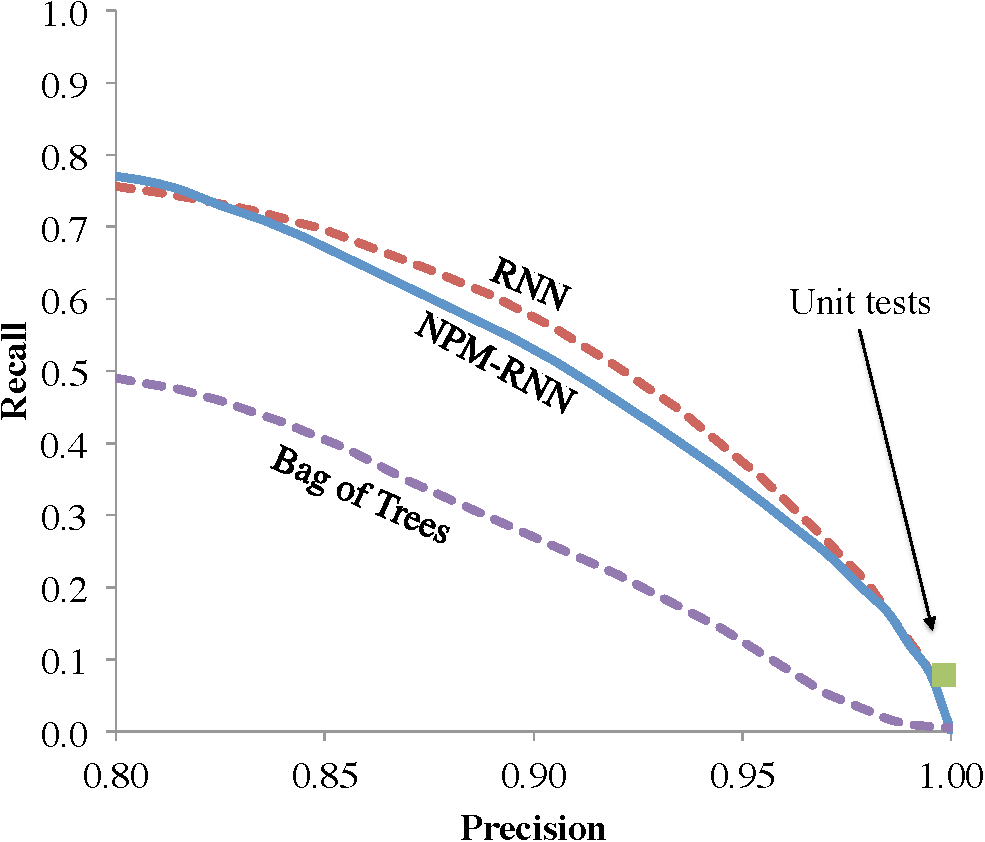
\includegraphics[width=0.3\textwidth]{img/force_mult_1}
\label{fig:fmHoc}
}
\subfigure[]
{
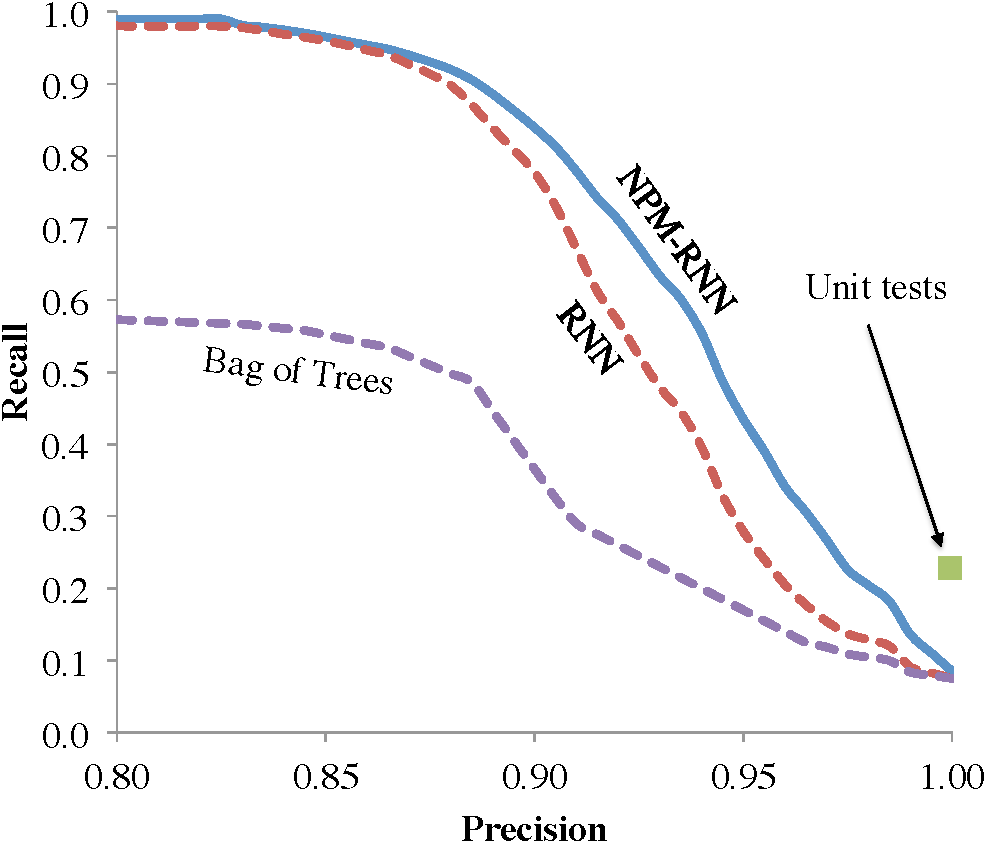
\includegraphics[width=0.3\textwidth]{img/force_mult_2}
\label{fig:fmNews}
}
\subfigure[]
{
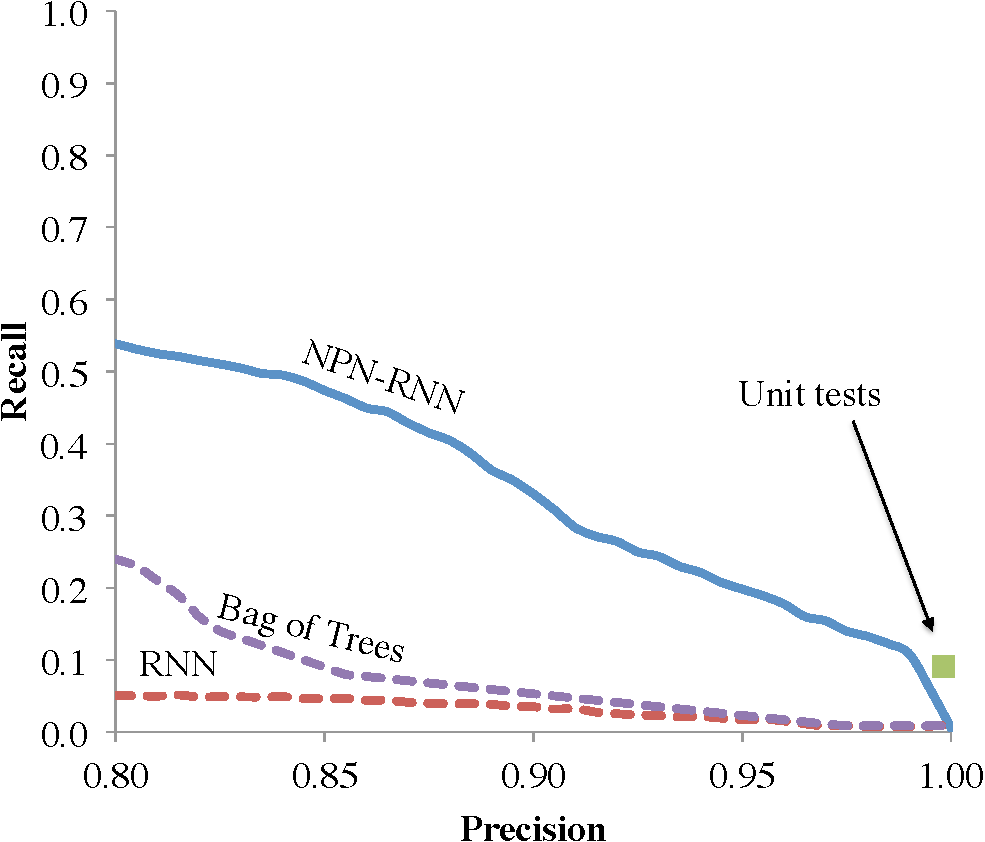
\includegraphics[width=0.3\textwidth]{img/force_mult_3}
\label{fig:fmMid}
}
\caption{
Recall of feedback propagation as a function of precision for three programming problems:
%Interplay between precision and the amount to which we can force multiply feedback for:
\subref{fig:fmHoc} $\Omega_1$,
 \subref{fig:fmNews} $\Omega_2$, and
  \subref{fig:fmMid} $\Omega_3$.  On each, we compare our NPM-RNN against the RNN
  method and two other baselines (bag of trees and unit tests).
 }
\label{fig:force}
\end{figure*}

We now use our program embedding matrices in the feedback propagation
application described in Section~\ref{sec:feedback}.  
The central question is: given a budget of $K$ human annotated programs (we set $K=500$), what fraction of 
unannotated programs can we propagate these annotations to using the labelled programs, and at what precision?  Alternatively, we are interested in the ``force multiplication factor'' --- the ratio of students who receive feedback via propagation to students to receive human feedback.
%In this experiment, we
%We ran force multiplication with a budget of $K$=500 human annotated programs. We can use the labelled programs and encodings to effectively propagate feedback. 

Figure~\ref{fig:force} visualizes recall and precision of our experiment on each of the three problems. The results translate to 214$\times$, 12$\times$ and 45$\times$ force multiplication factors of teacher effort for $\Omega_1$, $\Omega_2$ and $\Omega_3$ respectively while maintaining 90\% precision. The amount to which we can force multiply feedback depends both on the recall of our model and the size of the corpus to which we are propagating feedback. For example, though $\Omega_2$ had substantially higher recall than $\Omega_1$, in $\Omega_2$ the grading task was much smaller. There were only 6,700 unique programs to propagate feedback to, compared to $\Omega_1$ which had over 210,000. 
As with the previous experiment, we observe that 
for both $\Omega_1$ and $\Omega_2$, the NPM-RNN and RNN models perform similarly. However for $\Omega_3$, the NPM-RNN model substantially outperforms all alternatives.

In addition to the RNN, we compare our results to three other baselines: (1) Running unit tests, (2) a ``Bag-of-Trees'' approach and (3) $k$-nearest neighbor (KNN) with AST edit distances.  The unit tests unsurprisingly are perfect at recognizing correct solutions. However, since our dataset is largely composed of intermediate solutions and not final submissions (especially for $\Omega_1$ and $\Omega_3$), unit tests are not a particularly effective way to propagate annotations. 
%This is best expressed by the distribution of feedback shown in Figure~\ref{fig:whereWrong}, discussed further in the next paragraph.
The Bag-of-Trees approach, where we trained a Na\"{i}ve Bayes model to predict feedback conditioned on the set of subtrees in a program,
is useful
%we found the Naive Bayes probability of feedback, given the %collection of subtrees in a program 
%was notably useful 
for feedback propagation but we observe that it underperforms the embedding solutions on each problem. Moreover, we extended this baseline by amalgamating functionally equivalent code \cite{nguyen14}. Using equivalences found using similar amount of effort as in previous work, we are able to achieve 90\% precision with recall of 39\%, 48\% and 13\%, for the three problems respectively. While this improves the baseline, NPM-RNN obtains almost twice as much recall on all problems. Finally, we find KNN with AST edit distances to be computationally expensive to run and highly ineffective at propagating feedback --- calculating edit distance between all trees requires 20 billion comparisons for $\Omega_1$ and 1.5 billion comparisons for $\Omega_3$. Moreover, the highest precision achieved by KNN for $\Omega_3$ is only 43\% (note that the cut-off for the x-axis in Figure~\ref{fig:force} is 80\%) and at that precision only has a recall of 1.3\%. 

The feedback that we propagate covers a range of stylistic and functional annotations. To further understand the strengths and weaknesses of our solution, we explore the performance of the NPM-RNN model on each of the nine possible annotations for $\Omega_3$. As we see in Figure \ref{fig:whereWrong},
our model performs best on functional feedback with an average 44\% recall at 90\% precision, followed by strategic feedback and performs worst at propagating purely stylistic annotations with averages of 31\% and 8\% respectively.  Overall propagation for $\Omega_3$ is 33\% recall at 90\% precision. 


\begin{figure*}[t]
\centering
\subfigure[]
{
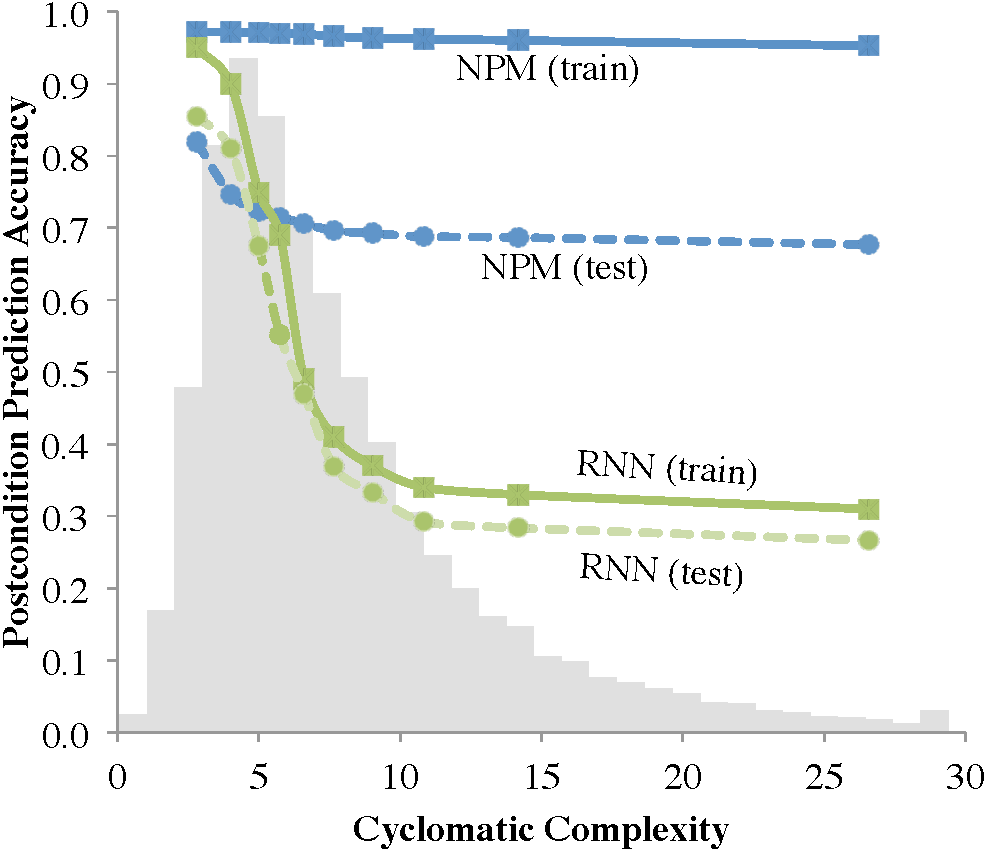
\includegraphics[width=0.29\textwidth]{img/prediction_acc_v_cyclomatic}
\label{fig:cycloPost}
}
\subfigure[]
{
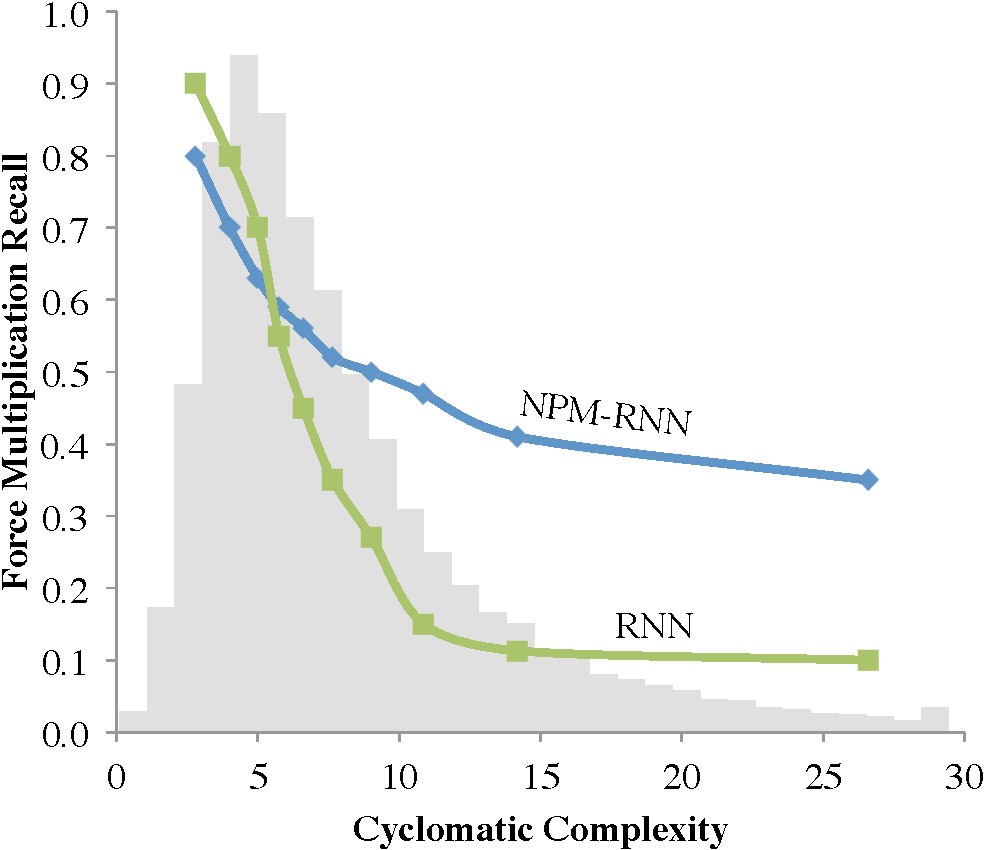
\includegraphics[width=0.29\textwidth]{img/forcemulti_v_cyclomatic}
\label{fig:cycloFm}
}
\subfigure[]
{
\raisebox{4mm}{
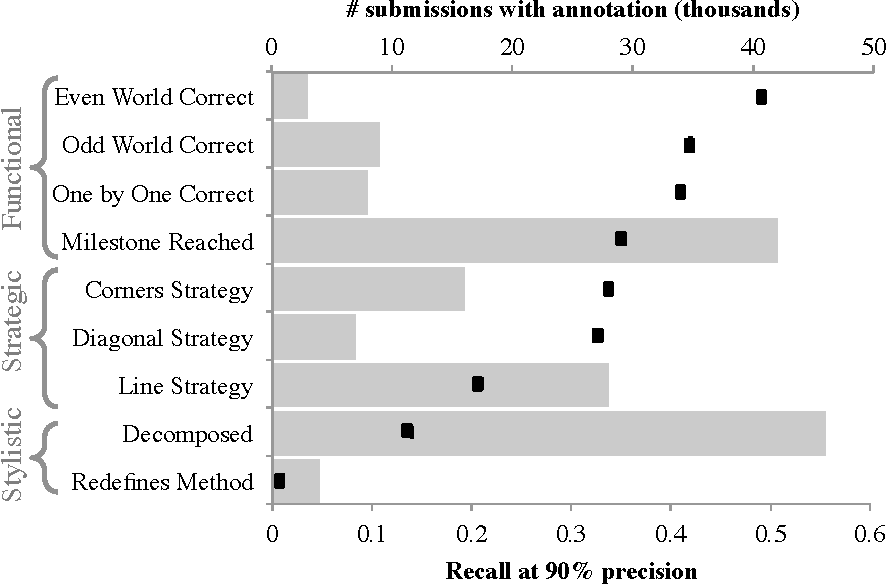
\includegraphics[width=0.33\textwidth]{img/force_mult_bystrategy}
}
\label{fig:whereWrong}
}
\caption{
\subref{fig:cycloPost} NPM and RNN postcondition prediction accuracy
as a function of cyclomatic complexity of submitted programs;
\subref{fig:cycloFm}
NPM-RNN and RNN
feedback propagation recall (at 90\% precision). Note that the ratio of human graded assignments to number of programs is much higher in this experiment than Figure~\ref{fig:force}; 
\subref{fig:whereWrong} A breakdown of the accuracy of the nonparametric model
by feedback type for $\Omega_3$ (black dots).  The gray bars histogram
the feedback types by frequency.
}
\label{fig:cyclomatic}
\end{figure*}


\subsection{Code complexity and performance}
The results from the above experiments are suggestive
that the nonparametric models perform better on more complex
code while the parametric (RNN) model performs better on simpler
code.  To dig deeper, we now look specifically into how our performance depends on the complexity of programs in our corpus
%We set out to better understand the nature of the matrices that we %learned and to do so devised a series of explorations. 
%Our first experiment was to understand how our ability to understand %programs, both predicting post conditions and propagating feedback %depended on the complexity of trees in our corpus. 
 --- a question that is also central to understanding how our models might apply to other assignments. We focus on submissions for $\Omega_3$, which cover a range of complexities, from simple programs to ones with over 50 decision points (loops and if statements). The distribution of \emph{cyclomatic complexity}~\cite{mccabe1976complexity}, a measure of code structure, reflects this wide range (shown in gray in Figures~\ref{fig:cycloPost},\subref{fig:cycloFm}). 
% We sort all submissions to $\Omega_3$ by cyclomatic complexity and bin them into ten groups of equal size. 
We first sort and bin all submissions to $\Omega_3$  by cyclomatic complexity into ten groups of equal size.
Figures~\ref{fig:cycloPost},\subref{fig:cycloFm} plot the results
of the postcondition prediction and force multiplication experiments run individually on these smaller bins (still using a holdout set, and a budget of 500 graded submissions).  
%The most striking result is the differences in performance for prediction of post-condition. 
While the RNN model performs better for simple programs (with cyclomatic complexity $\leq 6$), both train and test accuracies for the RNN degrade dramatically as programs become more complicated. On the other hand, while the NPM model overfits, 
it maintains steady (and better) performance in test accuracy 
as complexity increases. 
This pattern may help to explain our observations that the RNN is more accurate for force multiplying feedback on simple problems.


%A second experiment that we ran was to test how well our models were %able to represent program composition. If we assume that $f_Q =  M_A %\dot f_P$ and that $f_R = M_B \dot f_Q$ for two different programs %$A$ and $B$, it should hold that $f_R = M_b \dot M_A \dot f_P$. We %collected a corpus of five thousand programs that were composed of a subprogram $A$ followed by another subprogram $B$ (Compose-2). This corpus captures naturally occuring compositions. We than tested how well we were able to predict the postcondition of executing $A$ followed by $B$ on a given precondition, using their respective embeddings. The accuracy using the NP model for predicting the postcondition was 94\% when using the matrix for the root embedding. Using just $A$ and $B$ we could compute the postcondition with 92\% accuracy. When we tested programs that were composed of three subprograms, $A$ followed by $B$ followed by $C$ (Compose-3) accuracy dropped to 83\%. This ability to predict the result of composing programs was notably better using the NP embeddings than using the RNN embeddings. We also used this experiment to understand the utility of learning a joint model of matrix embeddings and state embeddings. We compared the accuracy of NP to the accuracy of NP-0, the same model just using its initialization which could be learned via ridge regression. Composition performance was notably worse for NP-0. This suggests that in the joint inference, we are able to learn an embedding of states that is more amenable to composition and thus is a more natural articulation of program functionality.



\section{Discussion}
In this paper we have presented a method for finding simultaneous embeddings of preconditions and postconditions into points in shared Euclidean space where a program can be viewed as a linear 
mapping between these points. 
These embeddings are predictive of the function of a program, and
as we have shown, can be applied to the the tasks of propagating teacher feedback. The courses we evaluate our model on are compelling case studies for different reasons. Tens of millions of students are expected to use Code.org next year,  meaning that the ability to autonomously provide feedback could impact an enormous number of people.  The Stanford course, though much smaller, highlights
the complexity of the code that our method can handle.
%We show the effectiveness of this model applied to the the tasks of propagating teacher feedback. The courses we test our experiment on are compelling case studies for different reasons. Code.org as tens of millions of students
%are expected to use the website next year meaning the ability to autonomously provide feedback could improve the educational experience of many students. The Stanford course, though a high quality curriculum is not taught outside of the university mainly because feedback cannot be delivered in a scaled way. However, while these are worthy applications the programs we analyzed were quite basic. In particular the data we looked at did not include user defined variables which made learning state space more straightforward. To incorporate user defined variables we would need to develop a more sophisticated state model. 

There remains much work towards making these embeddings more 
generally applicable, particularly for domains where we do not have
tens of thousands of submissions per problem or the programs are more complex. For settings where users can define their own variables it would be necessary to find a novel method for mapping program memory into vector space. An interesting
future direction might be to jointly find embeddings across multiple homeworks from the same course, and ultimately, to 
even learn  using arbitrary code outside of a classroom environment. To do so may require more expressive models. From the standpoint  of purely predicting  program output, the approaches described in this paper are not capable of representing arbitrary computation in the 
sense of the Church-Turing thesis.  However,
there has been recent progress in the deep learning community
towards models capable of simulating Turing machines~\cite{graves2014neural}. 
While this  ``Neural Turing Machines'' 
line of work approaches quite a different problem
than our own, we remark that such expressive
representations may indeed be important for statistical
reasoning with arbitrary code databases.
%The utility of embeddings for a corpus of student solutions is not limited to propagating feedback. Having a program representation that is enables general machine learning tasks for example predicting future struggles and even student dropout. Moreover, many courses, including the ones analyzed record not just a student's final solution but also the series of submissions a student took to get there. The task of discovering patterns in these trajectories could be better posed using euclidean embeddings of partial solutions.


For the time being, 
feature embeddings of code can at least be learned using
the massive online education
datasets that have only recently
become available.  And we believe that these features will
be useful in a variety of ways --- not just in propagating 
feedback, but also in tasks such as  predicting future struggles and even student dropout.

%Feature learning holds great promise for assessment of student assignments at scale. For many mediums (eg text, images etc), there are unsupervised learning algorithms that can transform them into a euclidean space, especially given the substantial structure in a corpus of students solving the same problem.

%Other avenues for future work include: joint inference of embedding spaces across assignments, and learning richer models for embeddings and feedback propagation. In this paper we modelled the relationship between Hoare-triples as $f(Q) = M_A \dot f(P)$. While this model was simple and effective one could imagine that it would also be reasonable to embed matrices using $f(Q) = g_A(f(P))$ where $g_A$ is a multi-layered feed-forward network with weights specific to program $A$. It would be harder to interpret the meaning of a program, but the same mapping could be expressed with many fewer parameters.



\section*{Acknowledgments} 
We would like to thank Kevin Murphy, John Mitchell, Vova Kim, Roland Angst, Steve Cooper and Justin Solomon for their critical feedback and useful discussions. We appreciate the generosity of the Code.Org team, especially Nan Li and Ellen Spertus, who providing data and support. Chris is supported by NSF-GRFP grant number DGE-114747.
% also 

\part{Alternative Ideas and Future Work}

\chapter{Crowd Source Feedback}

Based on a paper: Tuned Models of Peer Assessment in MOOCs \cite{piech2013tuned}\\ \emph{International Conference on Educational Data Mining 2013.}

\vspace{7mm}

\begin{figure}[h!]
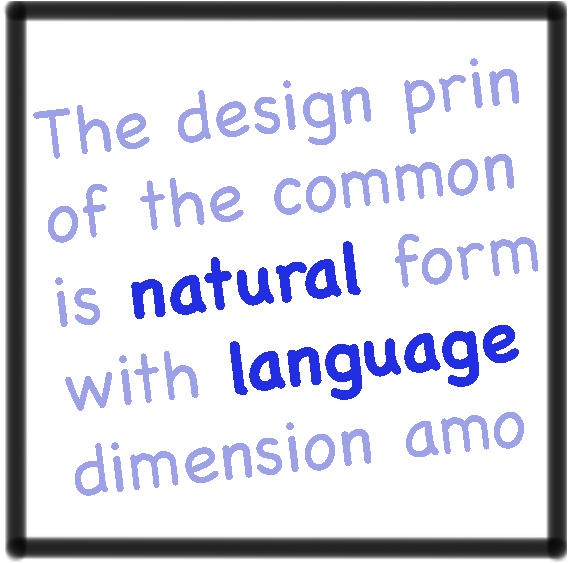
\includegraphics[width=0.2\textwidth]{img/assnType_5}
\end{figure}

\vspace{7mm}

Another angle into providing feedback at scale is to leverage the crowd of students to provide feedback to one another. Peer assessment --- which has been historically used 
for logistical, pedagogical, metacognitive, and affective benefits (\cite{sadler06})
%to improve student 
%involvement and expose learners to alternative solutions 
 --- 
could potentially be used in computer science classes. Because students have cognitive abilities that scale with the difficulty of the course, the ability of peers to provide feedback is generally independent of the richness of an assignment. Thus not only could peer grading be a way to provide feedback on the sort of programming assignments we have seen so far, it is also applicable to free form computer science projects.

In massive open online courses (MOOCs), peer grading serves as a critical tool for scaling the grading of complex, open-ended assignments to courses with tens or hundreds of thousands of students. But despite promising initial trials, it does not always deliver accurate results compared to human experts. In this chapter, we develop algorithms for improving peer grading accuracy on real data with 63,199 peer grades from Coursera's HCI course offerings --- the largest peer grading networks analysed to date. As a corrolary we relate grader biases and reliabilities to other student factors such as student engagement, performance as well as commenting style. We also show that our model can lead to more intelligent assignment of graders to gradees.

\begin{figure}
\begin{center}
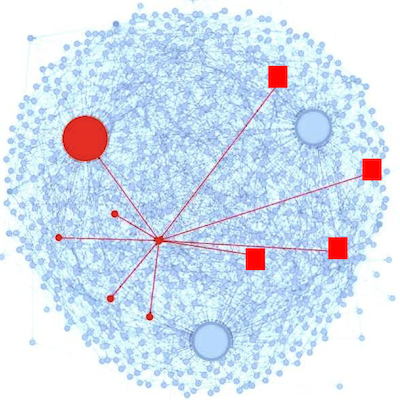
\includegraphics[width=.6\textwidth]{img/assn5GradingGraph_color}
\end{center}
\caption[Example peer grading network]{Peer-grading network: Each node is a learner with edges depicting
who graded whom. Node size represents the number of graders for that student.
The highlighted learner shown above graded five students (circular nodes)
and was in turn graded by four students (square nodes). }
%Assn 5 peer grading graph. Each node is a learner (size represents number of graders). One example learner is highlighted. She graded circle nodes and was graded by square nodes.}
\label{fig:gradingnetwork}
\end{figure}


Initial MOOC-scale peer grading experiments have shown
promise. A recent offering of an online Human Computer Interaction (HCI) course demonstrated that on average, student grades in a MOOC exhibit agreement with staff-given grades \cite{kulkarni13}. Despite their
initial successes, there remains much room for improvement. It was estimated that 43\% of student submissions in the HCI
course were given a grade that fell over 10 percentage points
from a corresponding staff grade, with some submissions up
to 70pp from staff given grades. Thus a critical challenge lies
in how to reliably obtain accurate grades from peers. 
%A long history of research into the application of statistical models to 
%peer assessment, exemplified by  Goldin et al.~\cite{goldin11,goldin12} suggests that we may be able to improve our accuracy by modeling at the very least grader bias.

In this chapter, we present the largest peer grading networks analysed to date with over $63,000$ peer grades. Our central contribution is to use this unprecedented volume of peer assessment data to extend the discourse on how to create an effective grading system. We formulate and evaluate  intuitive probabilistic peer grading models for estimating submission grades as well as grader biases and reliabilities, allowing ourselves to compensate for grader idiosyncrasies. Our methods improve upon the accuracy of baseline peer grading systems that simply use the median of peer grades by over $30\%$ in 
root mean squared error (RMSE).

In addition to achieving more accurate scoring for peer grading, we also show how fair scores
%(where each student gets a similar level of grade confidence)
(where our system arrives at a similar level of confidence about every student's grade)
can be achieved by maintaining estimates of uncertainty of a submission's grade.

Finally we demonstrate that grader related quantities in our statistical model such as bias and reliability
have much to say about other educationally relevant quantities. Specifically we explore summative influences: what variables correspond with a student being a better grader, and formative results: how peer grading affects future course participation. With the large amount of data available to us, we are able to perform detailed analyses of these relationships that would have been difficult to validate with smaller datasets.

Because peer grading is structurally similar in both MOOCs and traditional brick and mortar classrooms, these results shed light on best practices across both mediums. At the same time, our work helps to describe the unique dynamics of peer assessment in a very new setting --- one which may be part of a future with cheaper, more accessible education. 

\section{Datasets}\label{sec:datasets}
In this work, we use datasets collected from two 
consecutive Coursera offerings of Human Computer Interaction (HCI), taught by Stanford professor Scott Klemmer.
The HCI courses used a calibrated peer grading system~\cite{russell04} in order to assess weekly student submissions for
assignments which covered a number of different creative design tasks
for building a web site. Calibration required students to correctly assess a training submission before they were allowed
to grade other students' submissions. On every assignment,
each student evaluated five randomly selected submissions
(one of which was a ``ground truth'' submission, discussed below) based on a rubric, and in turn, was evaluated by four
classmates. The final score given to a submission was
determined as the median of the corresponding peer grades.\footnote{
Our description is somewhat of a simplification --- students also performed self-assessments and were given
the higher of the median and their self grade provided that the two were within five percentage points of each other.
We did not consider self assessments in this work.}
Peer grading was anonymized so that students could not see
who they were evaluating, or who their evaluators were.
See Kulkarni et al.~\cite{kulkarni13} for details of the peer grading system.

After the first offering (HCI1), the peer grading system was refined in several ways. Among other things, HCI2 featured a modified rubric that
addressed some of the shortcomings of the original peer grading scheme. Additionally, peer graders were divided into language groups
(English and Spanish) to address concerns of being graded
by a non-native speaker as well as the observed ``patriotic
grading effect''~\cite{kulkarni13}.  
Counting just those who submitted at least one assignment 
in the English offerings of the class, there were 3,607 students 
from the first offering (HCI 1) and 3,633 students
from the second offering (HCI 2).  These students came from diverse backgrounds
 (with a majority of students from outside of the United States). 
 Collectively, these 7,240 students from around the world 
created 13,972 submissions, receiving 63,199 peer grades in total. See Table~\ref{tab:datasets} for a summary of the dataset.
In our work, we used the data
from HCI2 as a hold out set. We formulated our models based only on exploratory experiments performed using the HCI1 dataset, testing on the second HCI
class only after having finalized our theories about which
models were useful.

\begin{table}[t!]
\caption[Tuned peer grading dataset summary]{Data Sets}
\begin{center}
\begin{tabular}{rcc}
\hline
 &  First HCI & Second HCI \\
\hline
Students  & 3,607  &  3,633\\
Assignments & 5  &  5\\
Submissions & 6,702 & 7,270\\
Peer Grades & 31,067  &  32,132\\
\hline
\end{tabular}
\end{center}
\label{tab:datasets}

\end{table}


The software for the peer grading framework
used by the HCI courses was designed to accommodate experimental validation of peer grading. A small number (3-5)
of submissions for each assignment were marked as ``ground
truth'' and were then graded by the course staff. Since there
were only a few ground truth submissions and each student
graded at least one per week, the ground truth submissions
were ``super-graded'' and had, on average, 160 assessments.
Of note, the students were not told that one of the submissions they were assigned to mark belonged to the ground truth set. For
example, Figure~\ref{fig:gradingnetwork} shows the network of gradee-grader relationships on Assignment 5 of HCI1, where the three super-graded ground truth submissions are clearly visible. %\Jon{Say why evaluation is nontrivial?}
\section{Probabilistic models of peer grading in MOOCs}
The ideal peer grading system for a MOOC should satisfy the following desiderata: it should (1) provide
highly reliable/accurate assessment, (2) allocate a balanced
and limited workload across students and course staff, (3)
be scalable to class sizes of tens or hundreds of thousands
of students, and (4) apply broadly to a diverse collection of
problem settings. 
In this section we discuss a number of ways to formulate a
probabilistic model of peer grading to address these desiderata. The models 
that we introduce allow for
us to algorithmically compensate for factors such as grader
biases and reliabilities while maintaining estimates of uncertainty in a principled way. 


Through our paper, we will use the following notation.
We refer to the collection of all submissions to a homework assignment as $U$, and specific submissions
indexed as $u\in U$.  We assume in this paper that each student corresponds to a unique homework submission
per assignment, and thus refer to students (users) and submissions interchangeably.
The collection of all graders is denoted by $G$, and specific graders
by $v\in G$.   Note that graders are themselves students with submissions.
Finally, we use the notation $v\rightarrow u$ to mean that grader $v$ grades submission $u$.  For example,
the set $\{u\,:\,v\rightarrow u\}$ refers to the collection of submissions graded by a single student $v$.

Our models assume the existence of the following quantities which are either observed or 
latent (unobserved) variables which we wish to estimate.
\begin{itemize}
\item {\bf True scores:}
We assume that every submission $u$ is associated with a \emph{true underlying
score}, denoted $s_u$, which is unobserved and to be estimated. 
\item {\bf Grader biases:}
Every grader $v$ is associated with a bias, $b_v\in \reals$.  These bias
variables reflect a grader's tendency to either inflate or deflate her assessment by a certain
number of percentage points.  
\item {\bf Grader reliabilities:}
We also model grader reliability, $\tau_v \in \reals^+$, reflecting how close on average
a grader's peer assessments tend to land near the corresponding submission's true score after having
corrected for bias.  In the models
below, $\tau_v$ will always refer to the \emph{precision}, or inverse variance of a normal distribution.
%\item {\bf Coupling factors:}
%We finally consider a \emph{coupling factor} $W$ which
%models the degree to which a grader's grade is correlated with the grades
%that he assesses as a grader. \Jon{not sure if this will appear in the final paper}
\item {\bf Observed grades:} 
Finally, $z^v_u\in \reals$ is the observable score given by grader $v$ to submission $u$.
The collection of all observed peer grades is denoted as  $Z=\{z^v_u\}$.
\end{itemize}
\begin{figure*}
\begin{center}
\subfigure[]{
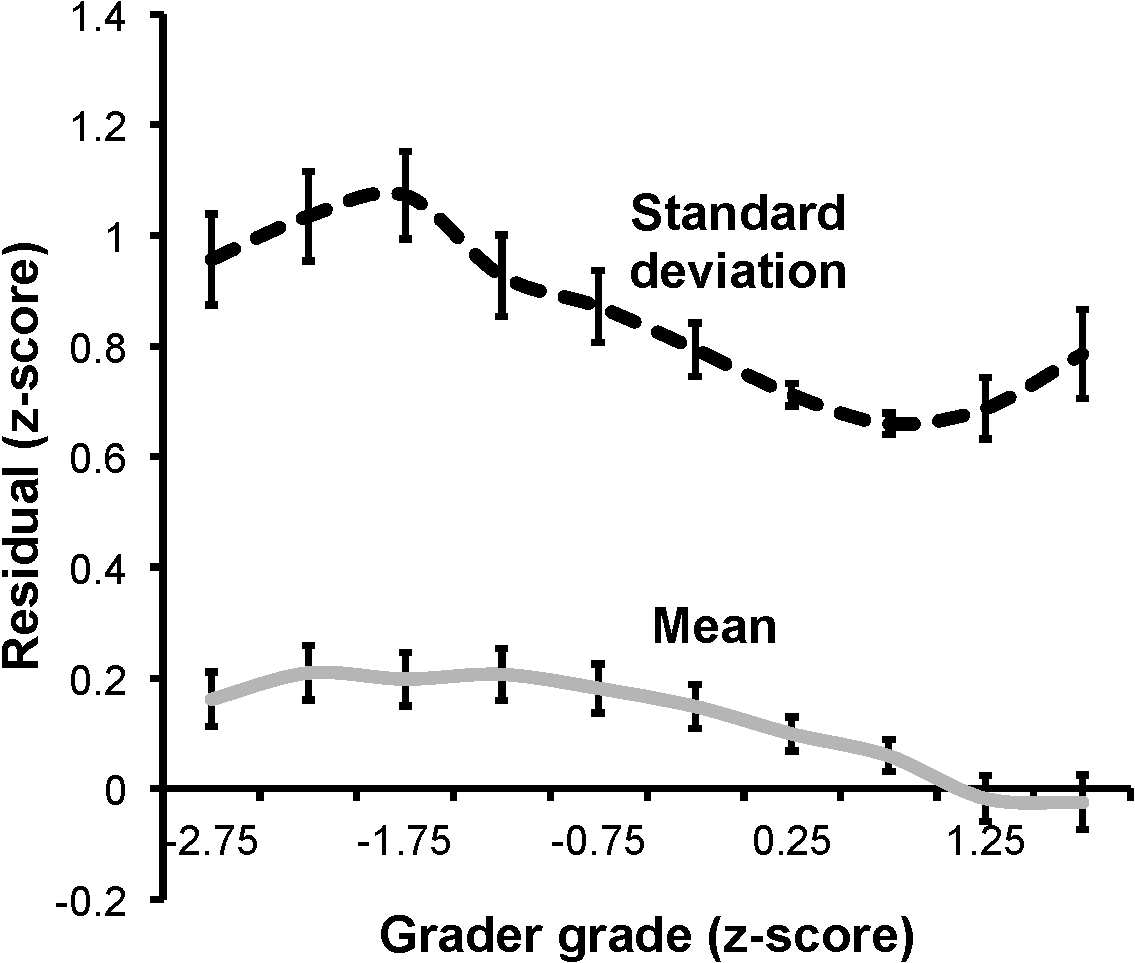
\includegraphics[width=.30\textwidth]{img/gradergrade_v_residual.pdf}
\label{fig:gradergrade_v_residual}
}\;\;
\subfigure[]{
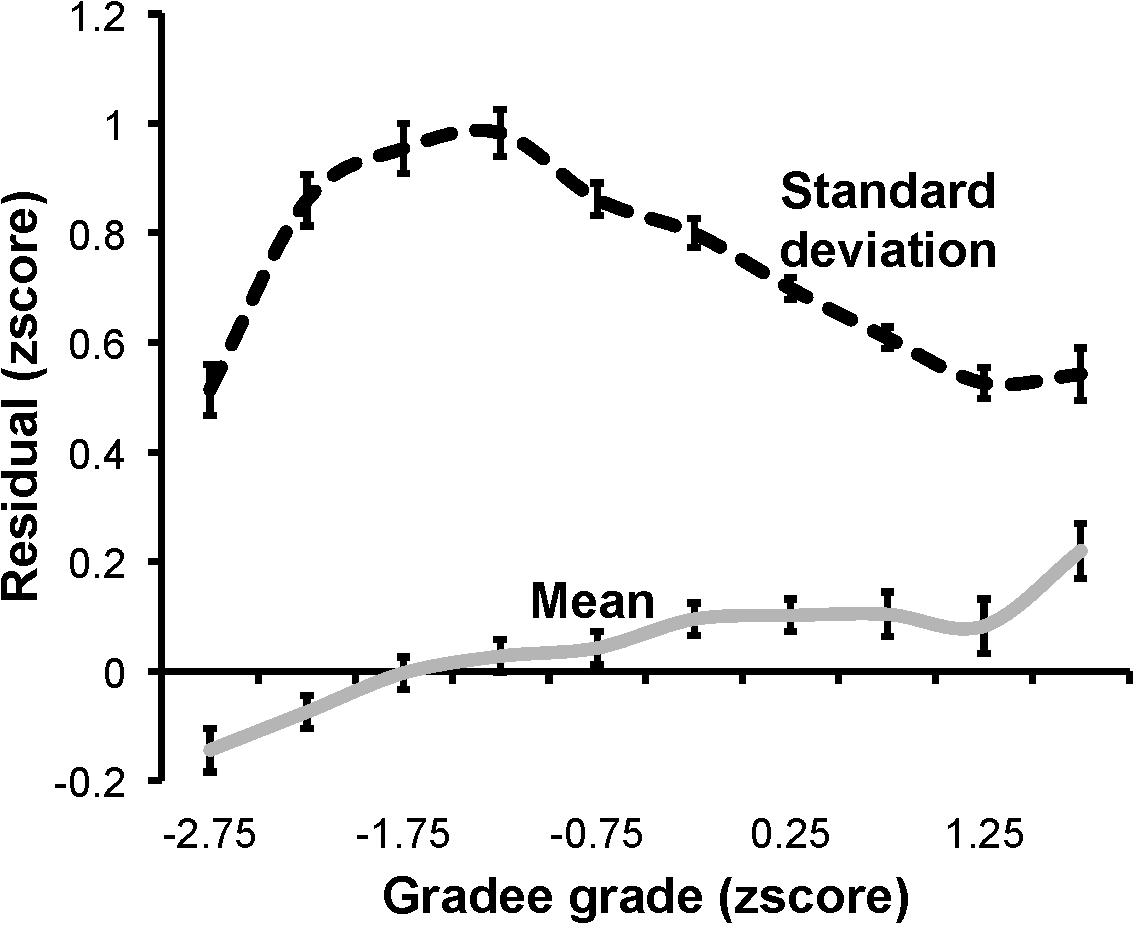
\includegraphics[width=.30\textwidth]{img/gradeegrade_v_residual.pdf}
\label{fig:gradeegrade_v_residual}
}\;\;
\subfigure[]{
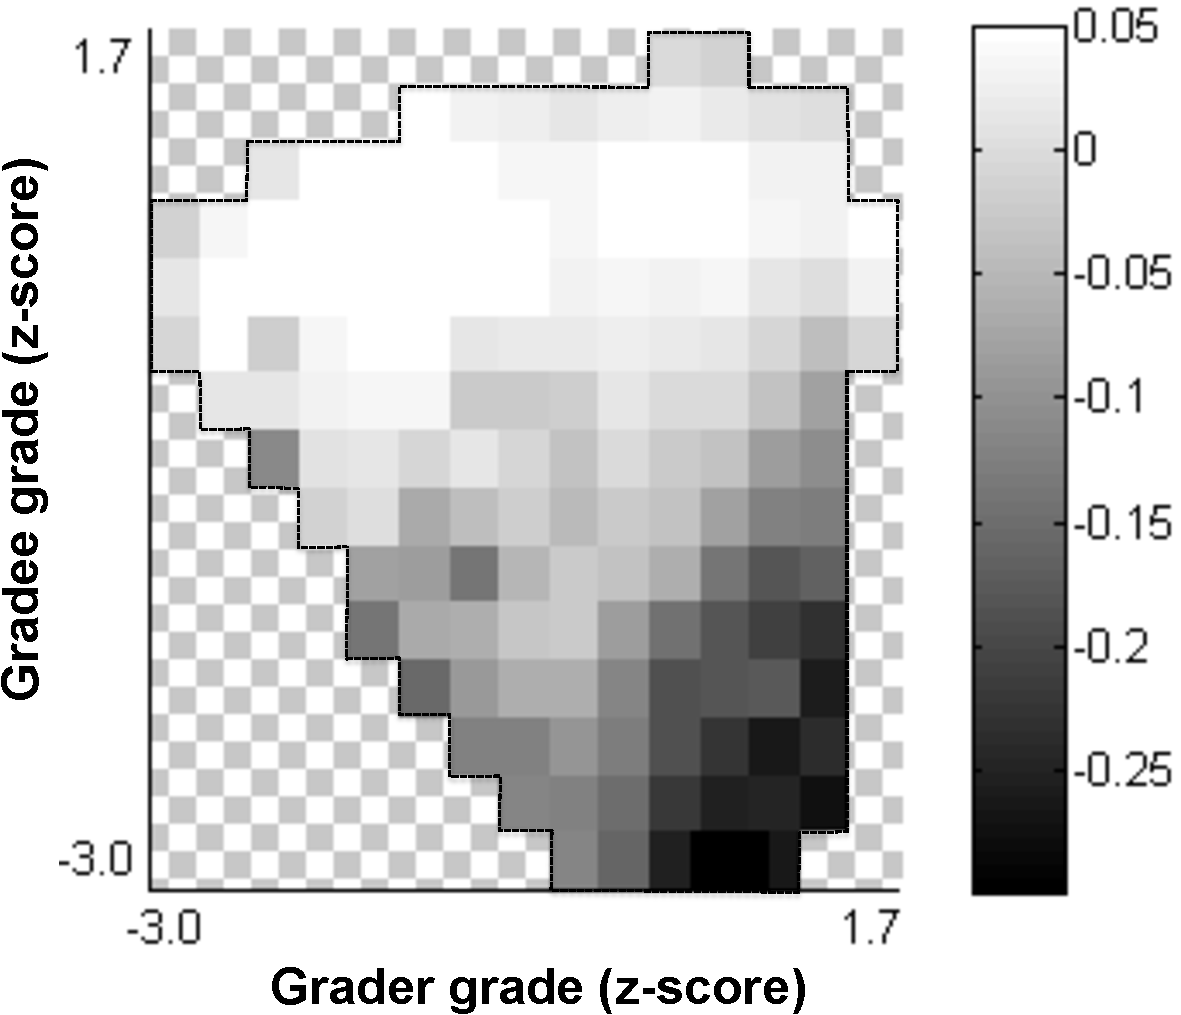
\includegraphics[width=.30\textwidth]{img/grader_v_gradeebias_transparent.pdf}
\label{fig:gradergradee}
}
\end{center}
\caption[Relationship between grades received and grades given]{%Relationship between grading performance  and
%homework performance of graders and gradees:
\subref{fig:gradergrade_v_residual} The relationship between a grader's homework performance (her grade)
and statistics (mean/standard deviation) of grading performance (residual from true grade).
\subref{fig:gradeegrade_v_residual} The relationship between a gradee's homework performance against statistics of assessments
for her submissions.
\subref{fig:gradergradee} Visualization of all three variables simultaneously, where intensity reflects
the mean residual $z$-score.  Empty boxes mean that there is not enough data available to compute a reliable estimate.
%We explored how grader scores and gradee scores impacted both the mean of a peer grades residual (bias) and the standard deviation (precision).
%color = mean residual z-score for each bucket
}
\label{fig:graders}
\end{figure*}

\subsection{Models}
Below we present, in order of increasing complexity, three statistical models that we have found to be particularly effective.

\paragraph{Model \PGone (Grader bias and reliability)}
%In our first model, we include grader biases and reliabilities.
Our first model, \PGone puts prior distributions over the latent variables and
assumes for example that while an individual grader's bias may be nonzero,
the average bias of many graders is zero.
Specifically, 

{\footnotesize
\begin{align*}
\mbox{(Reliability)}\; \tau_v &\sim  \mathcal{G}(\alpha_0,\,\beta_0) \;\mbox{for every grader $v$},\\
\mbox{(Bias)}\;b_v &\sim \mathcal{N}(0,\,1/\eta_0) \;\mbox{for every grader $v$},\\
\mbox{(True score)}\;s_u&\sim \mathcal{N}(\mu_0,\,1/\gamma_0)  \;\mbox{for every user $u$, and}\\
\mbox{(Observed score)}\;z^v_u &\sim \mathcal{N}( s_u + b_v,\, 1/\tau_v ), \\
       &\qquad \;\mbox{for every observed peer grade.} 
\end{align*}
}

$\mathcal{G}$ refers to a gamma distribution with fixed hyperparameters $\alpha_0$, $\beta_0$, while
$\eta_0$, and $\gamma_0$ are hyperparameters for the priors over biases and true scores, respectively.
In our experiments, we also consider a simplified version of
Model \PGone in which the reliability of every grader is fixed
to be the same value. We refer to this simpler model in which
only the grader biases are allowed to vary as \PGonebias. 

%We now describe two variations of Model \PGone which we have found to be useful.
%\Jon{probably should have a quick note on other potential ways to formulate this model
%and why they don't work as well}

\paragraph{Model \PGtwo (Temporal coherence)}
The priors for reliability and bias can play a particularly important role in the above model
due to the fact that we typically only have about 4-5 grades to estimate the bias and reliability
of each grader.  A simple way to obtain more data per grader %, however, 
is to leverage observations made about the grader from previous assignments.  To pose a model, we must understand the relationship
of a grader's bias and reliability at homework $T$ to that at homework $T'$.  Is it the same or does it change over time?

To answer this question, we examine the correlation between the estimated biases from Model \PGone using 
the HCI1 dataset (see Section~\ref{sec:datasets}). Between consecutive assignments, 
a grader's biases have a Pearson correlation of 0.33 which
represents a utilizable consistency. Grader reliability, on the other hand, has a low correlation.
We therefore posit Model \PGtwo which allows for grader biases
at homework $T$ to depend on those at homework $T-1$ (and implicitly, on all prior homeworks).   Specifically, Model \PGtwo assumes:


{\footnotesize\allowdisplaybreaks
\begin{align*}
\tau_v^{(T)} &\sim  \mathcal{G}(\alpha_0,\beta_0) \;\mbox{for every grader $v$},\\
b_v^{(T)} &\sim \mathcal{N}(b_v^{(T-1)},1/\omega_0) \;\mbox{for every grader $v$},\\
s_u^{(T)}&\sim \mathcal{N}(\mu_0,1/\gamma_0) \; \mbox{for every user $u$, and}\\
z^{v,(T)}_u &\sim \mathcal{N}( s_u^{(T)} + b_v^{(T)}, 1/\tau_v^{(T)} ), \\
       &\qquad \;\mbox{for every observed peer grade.} 
\end{align*}
}

%\Jon{I also forwarded bias posterior confidence values}
Model \PGtwo requires that we normalize grades across different homework assignments to a consistent scale. In our
experiments, for example, we have noticed that the set of grader
biases had different variances on different homework assignments. Using
a normalized score ($z$-score), however, allows us to propagate a student's underlying bias while remaining robust to assignment
artifacts.

Note that while a model which captures the dynamics of true scores and reliabilities across assignments can be similarly imagined,
we have focused only on the dynamics of bias for this work (which %, as we discuss in Section~\ref{sec:experiments}, contributes
contributes the most towards improved accuracy while still being equitable). 
%Moreover, we observed a particularly strong temporal correlation between student's grades (0.46 pearson coefficient) however, we decided that it might be %contentious if a student is not given a clean slate on each homework.
%\begin{figure}[t*]
%\begin{center}
%\subfigure[]{
%\fbox{\qquad\qquad}
%}
%\subfigure[]{
%\fbox{\qquad\qquad}
%}
%\end{center}
%\caption{Evolution of grader bias from homework to homework}
%\label{fig:biasevol}
%\end{figure}
%Write out a few versions of the model. (and in words what the assumptions are)
%\begin{itemize}
%\item Baseline model
%\item Model with reliability
%\item Model with bias and reliability
%\item Temporal model with bias
%\item Need to explain the "semi supervised thing"
%\end{itemize}

\paragraph{Model \PGthree (Coupled grader score and reliability)}
%One of the things that sets peer grading apart from crowdsourcing 
         %\Jon{crowdsourcing hasnt been mentioned yet. This might be a confusing reference} 
%is that the 
A unique aspect of peer grading is that graders are themselves
students with submissions being graded. %, whereas with typical crowdsourcing settings, there is a dichotomy between the labelers
%and the items being labeled.  
Consequently, it is of interest to understand and model the relationship between
one's grade and one's grading ability --- 
for example, knowing that a student
scored well on his assignment may be cause for placing more
trust in that student as a grader, and vice versa. 

In Figure~\ref{fig:graders}, we show
experiments exploring the relationships between the grader
specific latent variables. In particular, we observe
that high scoring students tend to be somewhat more reliable as graders (see details of the experiment in 
Section~\ref{sec:experiments}). Model \PGthree formalizes this
intuition by allowing the reliability of a grader to depend on
her own grade, and assumes the following:

{\footnotesize\allowdisplaybreaks
\begin{align*}
b_v &\sim \mathcal{N}(0,\,1/\eta_0) \;\mbox{for every grader $v$},\\
s_u&\sim \mathcal{N}(\mu_0,\,1/\gamma_0)  \;\mbox{for every user $u$, and}\\
z^v_u &\sim \mathcal{N}\left( s_u + b_v,\, \frac{1}{ \theta_1 s_v+ \theta_0 } \right),\\
       &\qquad  \;\mbox{for every observed peer grade.} 
\end{align*}
}

Note that Model \PGthree extends\PGone by introducing new dependencies, allowing us to use a student's submission
score to estimate her grading ability.
At the same time Model \PGthree is more constrained, forcing grader reliability to depend on a single parameter
instead of being allowed to vary arbitrarily, and thus prevents our model from overfitting.

\paragraph{Ethics and Incentives} 
%Predictions made by our probabilistic models can be used as
%scoring mechanisms in a MOOC by taking the score of a submission to
%be the model prediction instead of, for example, the median 
%of peer grades.
%However, 
If we are to use probabilistic inference to score students in a MOOC,
the end goal could not simply be to optimize for accuracy.
We must also consider fairness when it comes to deciding
what variables to include in the model. It might be tempting, for 
example, to include variables such as race, ethnicity and gender into a model for better accuracy, but almost everyone
would agree that these factors could not be fairly used within a
scoring mechanism even if they improved prediction accuracy. Another 
example might be to model the temporal coherence of student grades (we observe a particularly strong
temporal correlation between students' grades --- with 0.46 Pearson
coefficient --- of consecutive homework assignments). But incorporating this temporal coherence for students scores
into a scoring mechanism would
not allow for students to be given a ``clean slate'' on each
homework.

Model \PGthree allows for the inferred true score of a submission
to depend on graders' scores, which may seem contentious,
but the dependence is weak, only affecting the influence by
a particular grader on the final prediction, which is desirable. Interestingly, using the more complex scoring mechanism from Model \PGthree may 
in fact incentivize for good
grading. In particular, a student's grade is influenced by
how closely her assessments as a grader match those of other
graders who graded the same assignments. Consequently, by
allowing for student grades to depend on their performance
as graders, Model \PGthree used as a scoring mechanism may
incentive students to put more effort into grading.

\subsection{Inference and evaluation.}
Given a probabilistic model of peer grading such as those discussed above, 
we would like to infer the values of the unobserved variables such as the  true score of 
every submission, or the bias and reliability of each student as a grader.
Inference can be framed as the problem of computing the posterior distribution over the 
latent variables conditioned on all observed peer grades (e.g., $P(\{s_u\}_{u\in U}, \{b_v\}_{v\in G}, \{\tau_v\}_{v\in G}  \;|\; Z)$).
% \\
%&\propto \prod P(s_u; \gamma_0)\cdot \prod P(b_v; \eta) \cdot P(\tau_v; \alpha,\beta) \prod_{z^v_u\in Z} P(z^v_u | s_u,b_v,\tau_v).
%\end{align*}
%}

Computing this posterior is nontrivial, since all of the variables are correlated 
with each other.  For example, having good estimates of the biases of all of the graders to submission $u$ ($\{b_v: v\rightarrow u\}$)
would allow us to better estimate $u$'s true score, $s_u$.  However to estimate each bias $b_v$, we would have to have good estimates of the true scores of \emph{all} of the submissions graded
by $v$ ($\{s_u:v \rightarrow u\}$).
We must therefore reason circularly, in that --- if we knew
every submission's true scores, we would be able to easily compute posterior distributions
over grader biases (and reliabilities), but in order to estimate these biases, we must know
the true score of each submission.  

To address this apparent chicken and egg problem, we turn to simple approximate inference methods. 
In the experiments reported in Section~\ref{sec:experiments}, we use Gibbs sampling~\cite{geman84}, which produces
a collection of samples from the (approximate) desired posterior distribution. These samples can then be used to estimate various 
quantities of interest. For example, given
samples $s^1_u, s^2_u,\dots, s^T_u$ from the posterior distribution over 
the true score of submission $u$, we estimate the true score as: $\hat{s}_u \equiv \frac{1}{T} \sum_{t=1}^T s^t_u$. 
We can also use the samples to quantify the uncertainty of our prediction by estimating the variance of the samples from the
posterior, which we use in Section~\ref{sec:experiments} when we examine peer
grading efficiency. Note that while the ordinary Gibbs sampling algorithm can be performed in ``closed form'' for Models
\PGonebias, \PGone and \PGtwo, Model \PGthree requires numerical approximation due to the coupling of a submission's true
score $s_u$ with that of its grader, $s_v$. 
We discuss details in the Appendix.\footnote{See accompanying appendix at \url{www.stanford.edu/~cpiech/bio/papers/appendices/edm13_appendix.pdf}}  
Visually we observe rapid mixing for our Gibbs chains, and in the experiments shown in Section~\ref{sec:experiments}, we use
800 iterations of Gibbs sampling, discarding the initial 80 burn-in samples. 


%We show the Gibbs sampling approximate inference
%algorithm for a simplified version of Model \PGone (with constant reliability for all graders) in Algorithm~\ref{alg:gibbs}, 
%which alternates between two steps.  First it simulates the true score of submission $u$ by averaging the bias corrected peer grades
%and adding noise.  Then using the just-simulated true scores, it simulates the bias of each grader $v$ by averaging
%the difference between grades given by $v$ and corresponding true grades (and adding appropriate noise).
%By repeating the algorithm for many time steps and discarding the initial $B$ samples, we obtain samples
%from the desired (approximate) posterior distribution, from which we can estimate the quantities of interest, such
%as true grades, or grader bias.  For example, if we obtain samples $s^1_u, s^2_u,\dots, s^T_u$, from Gibbs sampling,
%then an estimate of the true score of submission $u$ is simply $\hat{s}_u \equiv \frac{1}{T} \sum_{t=1}^T s^t_u$.  
%We can also use the samples to quantify the uncertainty of our prediction by estimating posterior variance as:
%\begin{equation}\label{eqn:posteriorvariance}
%\var(s_u) \equiv \frac{1}{T-1} \sum_{t=1}^T (s^t_u - \hat{s}_u)^2,
%\end{equation}
%which will be useful in Section~\ref{sec:experiments} when we examine peer grading efficiency.

Expectation-maximization (EM) is alternative approximate inference approach, where we treat the true scores and grader biases as parameters
and then use an iterative coordinate descent based algorithm to obtain point estimates of parameters.  
In practice, we find that both the Gibbs and EM approaches behave
similarly.  In general EM has the advantage of being significantly faster while obtaining posterior credible intervals is more natural using Gibbs. On the peer grading dataset the two methods produce analogous results. For example, \PGone with Gibbs and EM have RMSE scores of 5.42 and 5.43 on the first dataset respectively and with Gibbs running in roughly 5 minutes and EM running in 7 seconds.
We refer the reader to the appendix for the full algorithmic details of Gibbs as well as EM.


\begin{table*}
\caption[Tuned peer grading accuracy]{Comparison of models on the two HCI courses}
\centering\footnotesize
\ra{1.3}
\begin{tabular}{@{}rcccccccccccc@{}}
\toprule[1.5pt]
& \multicolumn{5}{c}{HCI 1} & \phantom{abc}& \multicolumn{5}{c}{HCI 2} \\
\cmidrule{2-6} \cmidrule{8-12} 
& Baseline & \PGonebias & \PGone & \PGtwo & \PGthree &&                                    Baseline & \PGonebias & \PGone & \PGtwo & \PGthree  \\ \midrule
RMSE & 7.95 & 5.42 & 5.40 & 5.40 & {\bf 5.30}                  && 6.43 & 4.84 & 4.81 & 4.75 & {\bf 4.73} \\
\% Within 5pp &  51& 69& 69& {\bf 71} & 70                     && 59& 72& 73& 73 & {\bf 74} \\
\% Within 10pp & 81& 92& 94& 94& {\bf 95}               && 88& 96& 96& {\bf 97} & {\bf 97} \\
Mean Std & 7.23& 5.00& 4.96& 4.92& {\bf 4.77}           && 6.19& 4.57& {\bf 4.52} & 4.53 & {\bf 4.52} \\
Worst Grade & -43& -34& {\bf -30} & -32& {\bf -30}             && -36& -26& -26& {\bf -25} & -26\\
\bottomrule[1.5pt]
\end{tabular}
\label{tab:results}
\end{table*}

\paragraph{Evaluation}
To measure peer grading accuracy, we repeatedly simulate
what score would have been assigned to each ground truth
submission had it been peer graded. Our evaluation of how
well we would have graded a single ground truth submission
uses a two step methodology (based on the evaluation method of~\cite{kulkarni13}): (1) We run inference using
all of our data, except the peer grades of the ground truth
submission being evaluated. This gives us an estimate of each grader's biases and reliabilities as well as model
priors that were independent of the submission being evaluated. 
(2) We run simulations where we sampled four student
assessments randomly from the pool of peer grades for the
ground truth submission, estimate the submission's
grade using the sample of assessments and recorde the
residual between our estimated grade and the ``true'' grade.
For each ground truth submission we run 3000 such simulations, from which we report the RMSE, the number of simulations which fell
within five, and ten percentage points of the true score, the
average standard deviation of the errors over each ground
truth and the worst misgrade that the simulations produced.

An interesting issue is whether one should consider the ``true''
grade of a ground truth submission to be the score given by
the staff, or the consensus from the hundreds of students
that assessed the submission. For our datasets, we believe
that the discrepancy between staff grade and student consensus typically results from ambiguities in the rubric and
elect to use the mean of the student consensus on a ground
truth submission as the true grade. One interesting observation that came from our exploration: peer graders in our
datasets have a tendency to grade towards the mean, inflating
grades for low-scoring submissions and deflating grades for
high-scoring submissions. % \Jon{show a plot?}
 We remark that
while our experiments were run in an ``unsupervised'' fashion, it would be reasonable to use staff grades
in the training process in order to encourage the model to
place more trust in students who consistently grade like the
instructors.

We compare each of our probabilistic models to the grade
estimation algorithm used on Coursera's platform. In the
baseline model, the score given to students is the median of
the four peer grades they received. Specifically, the baseline
estimation does not take into account individual grader's
biases and reliabilities. Nor does it incorporate prior knowledge about the distribution of true grades. 

\section{Experimental results}\label{sec:experiments}


\begin{figure*}
\begin{center}
\subfigure[]
{
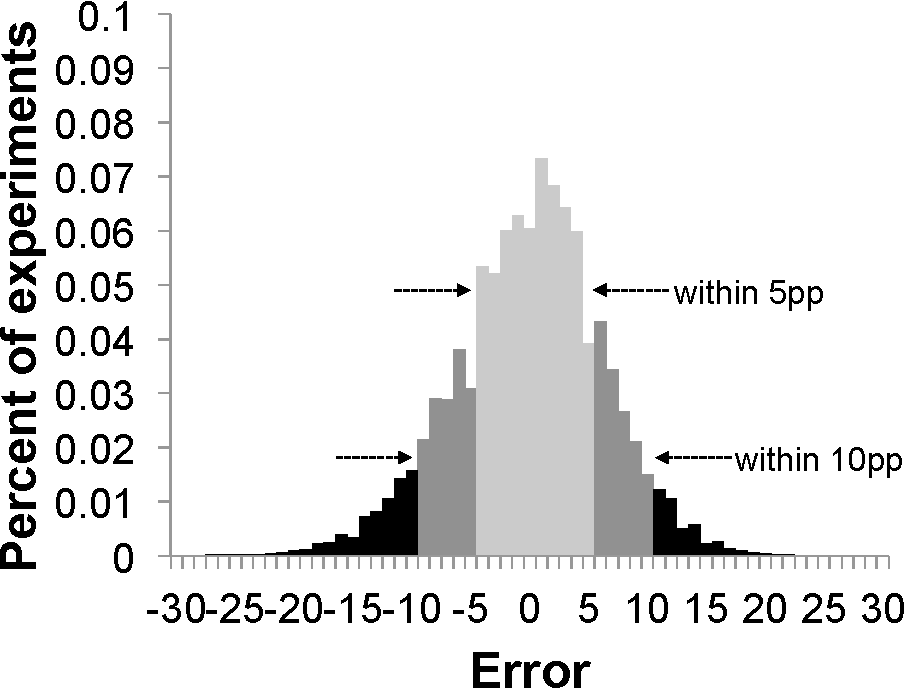
\includegraphics[width=.44\textwidth]{img/baseline.pdf}
\label{fig:baseline}
}
\subfigure[]
{
\includegraphics[width=.44\textwidth]{img/histogram.pdf}
\label{fig:improved}
}
\end{center}
\caption[How the histogram of errors changes]{
\subref{fig:baseline} Histogram of errors made using the baseline (median) scoring mechanism. 
 \subref{fig:improved} Histogram of errors using \PGthree.  
 }
\label{tab:predacc}

\end{figure*}

\subsection{Accuracy of reweighted peer grading}
Using probabilistic models leads to substantially higher grading accuracy. In our experiments we are able to reduce the
RMS error on our prediction of the ground truth grade by
33\% from 7.95 to 5.30. Similarly, on the second offering of
the course we were able to reduce error by 31\% from 6.43
to 4.73. For the second offering, this means that the number of students who received grades within 10 percentage
points (pp) of their grade increased from 88\% to 97\%. Figures~\ref{fig:baseline},~\ref{fig:improved} show the effect of using Model~\PGthree
as a scoring mechanism on the histogram of grading errors and Table~\ref{tab:results} shows the
complete results for each model. Due to course improvements, we observe that students
in HCI2 were significantly more consistent as graders compared to students in HCI1. However, we remark that every
one of our models run on HCI1 outperforms the baseline
grading system run on HCI2 with respect to every metric,
indicating that the best gains in peer grading are likely to
come from both an improved class design as well as statistical modeling.

Our results show that Models \PGthree (with coupled grader score and
reliability) and \PGtwo (with temporal coherence) yield the best results,
with Model \PGthree outperforming the other models with respect to most metrics.
But the single change that provides the
most significant gains in accuracy is obtained by estimating each grader's bias (Model \PGonebias). This simple
model is responsible for 95\% of our reduction in RMSE.
The other changes 
all contribute comparatively smaller improvements
to a more accurate model.

Our evaluation setup also allows us to test how accurate we would have been, had we had more than four grades per student. If the class had increased the number of grades that each student received to five (instead of four), our model could reduce RMSE error on the first and second offering of HCI to 4.19 and 4.36  respectively. 


Surprisingly while modeling grader bias is particularly effective, modeling grader precision does little to improve our
performance. To dig deeper into this result we test our
model on a synthetic dataset --- one generated exactly from
Model \PGone . When using this synthetic data with only
four grades per student it is difficult for the model to
correctly estimate grader reliability. Modeling variance for
each grader only seems to have a notable impact when students grade many assignments 
(more than 10). This experiment also suggests why \PGthree is more useful than \PGone .
Though \PGone contains more expressive power
than \PGthree, estimating only two parameters for grader reliability ($\theta_0$ and $\theta_1$) is more statistically tractable with only
four grades per student than estimating a reliability, $\tau_v$, for
each grader. 
%\Jon{Is there any way for us to attach numbers
%to this paragraph?}

\subsection{Fairness and efficiency in peer grading}
One of the advantages of using a probabilistic model for peer grading is
that we can obtain a belief distribution over grades (as opposed to a single score) for each student. These distributions give us a natural way of calculating how confident the model is when it predicts a grade for a student.
 %If these confidence results can be trusted, confidence values 
 The fact that the confidence results can be trusted
 open up the possibility of a more equitable allocation of graders. For example, at a given point midway through the peer grading process, our model may be highly confident
in its prediction for a given student's score, but very unsure in its prediction for another student. In this situation, to ensure that each student
gets fair access to quality feedback, we could reassign graders
to gradees such that submissions which have low-confidence
scores are given to more and/or better graders.

The first step towards more fair allocation of grades is to ask ourselves: how accurate are our
estimates of confidence?
For example, we would like to know how to interpret what it means in practice when our Bayesian
model is 90\% confident that its prediction of a learner's true score is within 10pp of the actual true score.

To better understand our confidence estimates, we run the following experiment: We first performed a large number of
peer grading simulations on ground truth. From each
simulation we calculate how confident our model is that
the grade it predict for the ground truth submission is
within 5\%, 7\%, and 10\%, of the true score, respectively. 
%We then sorted the predictions into confidence ranges. 
We then bin the estimated confidences into ranges 0-5\%, 5-10\%, etc.
%After collecting enough (>5,000)  predictions for all confidence ranges, 
After collecting over 5000 predictions per range, 
we test the pass rate of each range. For example, suppose we select four assessments of the same ground truth submission in a simulation. If our model reports a 72\% confidence --- based on those four assessments --- that our predicted grade is within 5pp
of the true score, we
add that estimate to the set of predictions in the 70\% to 75\%
confidence range. When we test this confidence range the example prediction ``passes'' if its estimate is in fact within 5pp of the ground truth score.

\begin{figure*}
\begin{center}
\subfigure[]
{
\includegraphics[width=.4\textwidth]{img/confidenceplot.pdf}
\label{fig:confidence}
}
\subfigure[]
{
\includegraphics[width=.36\textwidth]{img/piechart90.pdf}
\label{fig:piechart}
}
\end{center}
\caption[Model confidence vs accuracy]{
 \subref{fig:confidence}  A comparison of model confidence ($x$-axis) and actual success rate of predictions ($y$-axis), where
 being above the diagonal (dark bars) is better.
 \subref{fig:piechart} Number of submissions for which our model can declare ``confidence''
 after $K$ rounds of grading.
 }
\label{tab:predacc}

\end{figure*}

One worry is that our model might be overconfident about
its predictions even when wrong. However the results, shown in Figure~\ref{fig:confidence}, demonstrate
that our confidence estimates are on the conservative side ---
for example over 95\% of the time that our model claims it is between 90 and 95\% confident of a prediction, the model's estimate is correct. 

Since we have reason to believe that our confidence values are accurate, we can employ our posterior belief distributions to better allocate grades.  To understand how much benefit we could get out of improved grade allocation, we estimate at what point in the grading process we were confident about each submission's score. For each homework assignment, we simulate grading taking place in rounds. In the first round, we only include the first grade submitted by each grader (which may have been a ground truth grade). In the second round, we included the first two, etc. For each round we run our model using the corresponding subset of grades and count the number of submissions  for which we are over 90\% confident that our predicted grades were within 10pp of the student's true grade. 

After only two rounds of grading we are highly confident in our estimated grade for 15\% of submissions (this generally means that the submission has a grade close to the assignment mean, and has two similar grades from graders). Figure~\ref{fig:piechart} shows how the set of confident submissions grows over the grading rounds. Our experiment demonstrates a clear opportunity for grades to be reallocated as well as a pressing need for some submissions to get more grades. For 54\% of students, after all rounds, we are still unsure of their submission's true score.

\subsection{Graders in the context of the MOOC}
\begin{figure*}[t!]
\begin{center}
\subfigure[]{
\raisebox{3mm}{
\includegraphics[width=.44\textwidth]{img/time_v_residual.pdf}
}
\label{fig:time_v_residual}
}
\subfigure[]{
\includegraphics[width=.44\textwidth]{img/comments_v_residual.pdf}
\label{fig:comments}
}
\end{center}
\caption[Insight into peer graders]{
\subref{fig:time_v_residual}  Grader consistency (measured using standard deviation of grading residual) as
a function of time spent grading.
\subref{fig:comments} Commenting style (length of comment and sentiment polarity) as a function of grading residual.
}
\end{figure*}

Applying probabilistic models to peer grading networks allows us to increase our grade accuracy and better allocate
what submissions students should grade. Another product
of our work is an assignment --- with a belief distribution --- for a true score, grader bias and grader reliability
for each student. We can use this large dataset to derive
new understanding about peer grading as both a formative
and summative assessment. We focus our investigation on
two questions, (1) what factors influence  how well a student
grades? and (2) how does grading ability affect future class
performance in a MOOC?

\paragraph{Influential factors for grader ability} 
To explore what
factors influence how well a student grades we compare
grading residual (how far off a grader's score is from our
model estimated true score) to: time spent grading, grader grade, and gradee grade. 

Time spent grading shows a particularly interesting trend
(Figure~\ref{fig:time_v_residual}). As hypothesized, students that ``snap grade''
their peers' work (the students whose time spent grading has
a $z$-score of less than -0.30), are both unreliable (the
variance of their residuals is over 1 standard deviation
away from the gradee's true score) and tend to slightly
inflate grades. More surprising is that over the tens of
thousands of grades, there is a ``sweet spot'' of time spent
grading. Students who grade assessments with
a time that has a $z$-score of around -0.25 have significantly
lower residual standard deviations (with $p$-value < 0.001, diff = 0.3 standard
deviations) than students who take a long time to grade
(i.e., time spent grading has a $z$-score > -0.20). This sweet
spot is only visible when we look at normalized grading
times. For most assignments in the HCI class, the sweet
spot corresponds to around 20 minutes grading. This may reflect both that with any less time a grader does 
not have enough of a chance to fully examine her gradee's work, and that 
a long grading session may mean that the grader had trouble understanding 
some facet of the submission. % she is assessing.

Examining the relationship between grader grade, gradee
grade and how they affect the residual also shows a set of
notable trends. Graders that score higher on assignments
have close to monotonically decreasing biases (Figure~\ref{fig:gradergrade_v_residual}).
Getting a better grade on the homework in general makes
students more reliable graders; with the notable exception
that the students that get the best grades (+1.75 $z$-score)
are not as accurate as the students who do very well (+.75
$z$-score, $p$ = 0.04). The superlative submissions --- both the
best and the worst --- are the easiest to grade, and the submissions which are one standard deviation below the mean
are the hardest (Figure~\ref{fig:gradeegrade_v_residual}). Finally, our results show
that students are least biased when grading peers with
similar score (Figure~\ref{fig:gradergradee}). The best students significantly
downgrade the worst submissions and the worst students
notably inflate the best submissions.

In addition to numerical scores, graders were asked to provide feedback in the form of
free form text comments to their gradees. In order to understand the relationship between
grading performance and commenting style, we compare
grading residual against the comment length as well as sentiment polarity of the comment (Figure~\ref{fig:comments}).
To measure the polarity of a comment, we use the sentiment analysis
word list from~\cite{nielsen11} and implement a simple sentiment analyzer that returns a (normalized)
polarity score (positive or negative) %normalized score
proportional to the sum of word valences over the comment.
For both comment length and polarity, we filter out all non-English words.
We observe that comments that correspond to larger negative residuals are typically significantly longer,
suggesting perhaps that students write more about the weaknesses of a submission than strong points.
That being said, we observe that overall, the comments mostly range in polarity from neutral
to quite positive, suggesting that rather than being highly negative to some submissions,
many students make an effort to be balanced in their comments to peers.

\paragraph{Grader ability and future performance}
We also tested what signal grading ability has with predicting future participation.
Based on the theory that the best graders are
intrinsically motivated, we hypothesized that being a reliable grader would add a different dimension of information
to a student's engagement which we should be able to use to
better predict future engagement. We tested this hypothesis
by constructing a classification task in which we predict
whether a student would participate in the next assignment
(or conversely which students would ``drop out''). In addition to the student's grade, we experimented with including
grader bias and reliability as features in a linear classifier.
Our results (Figure~\ref{fig:roc}) show that including grader bias and
reliability improved our predictive ability by 5pp from an
area under the curve (AUC) score of 0.93 to an AUC of 0.98.
Properties about how a student grades, captures a dimension of their engagement which is missed by their assignment grade.

\begin{figure}[h]
\begin{center}

\includegraphics[width=.44\textwidth]{img/roc.pdf}
\label{fig:roc}
\end{center}
\caption[Predicting future class participation using peer grading]{ROC curve comparing performance (with linear SVM) at predicting future class participation given
a student's grade, bias, reliability or all three.
}
\end{figure}

\section{Related work}\label{sec:relatedwork}
The statistical models we present in this paper can be seen as part of a long tradition of models which have been proposed for the purposes of aggregating information from noisy human labelers or workers.
Many of these works adapt classical item-response theory (IRT) models~\cite{baker01} to the problem of
``grading without an answer key'' and appear in the literature from educational aptitude testing~\cite{johnson96,rogers10,mislevy99}, to
cultural anthropology~\cite{batchelder88,karabatsos03}, and more recently to HCI in the context of human computation and crowdsourcing~\cite{whitehill09}.
In educational testing, for example, Johnson~\cite{johnson96} and Rogers et al.~\cite{rogers10}
propose models for combining human judgements of essays.  %In contrast with peer grading,
These papers analyze \emph{dedicated human graders} who each evaluated hundreds
of essays, allowing for a rich model to be fitted on a per-grader basis.  In contrast, with peer
grading in MOOCs, each student only assesses a handful of assignments, necessitating more constrained models.



%You can bid on papers in the peer review process, specify keywords
%             and there are different topics that people have different expertises on,
%             whereas in peer grading, on some level, expertise is more one-dimensional
%      Grading an assignment is also likely to be less subjective than peer 
%             grading and numerical scores are likely to be more reliable (in some cases anyway).
%There is also citation link structure that is commonly drawn upon in suggesting
%                    peer reviewers.  But this is not applicable in MOOCs.
%What is good about this literature however is that they have focused
%             much effort on the actual (combinatorial) assignment problem.


%Our discussion has focused primarily on the peer grading system used in the 
%HCI course described by Kulkarni et al.~\cite{kulkarni13}.
%The results suggest that the shortcomings of peer grading for MOOCs are not fundamentally
%insurmountable and that by leveraging statistical tools appropriately we may be able to
%positively impact student experiences.


In a recent paper, and in a setting perhaps most similar to our
own, Goldin et al.~\cite{goldin11,ashley11,goldin12} use Bayesian models for peer grading in a smaller scale classroom setting. As in our
own work,~\cite{goldin12} posits a grader bias, and in fact incorporates
rubric-specific biases, but does not consider many of the
issues raised here such as grading task reallocation or the
relationship between grader bias and student engagement,
for example.

One of the central themes of the crowdsourcing literature, that of balancing label accuracy against labor cost, is one which MOOC peer grading 
systems must contend with as well.
In such problems, one typically receives a number of noisy labels (for example in an image tagging task)
and the challenge lies in (1) resolving the ``correct'' label (often discrete, but sometimes continuous) 
and (2) deciding whether to hire more labelers for a given task.  
Explosion of interest in recent years has led to widespread applications of crowdsourcing~\cite{bachrach12,kamar12}.
For example in image annotation, Whitehill et al.~\cite{whitehill09} present a method similar to our
own in which they model discrete ``true image labels'' as well as labeler accuracy.
While our work draws from the crowdsourcing literature, the problem of peer grading is unique in several ways. For example,
the fact that the graders are also gradees in peer grading is
quite different from typical crowdsourcing settings in which there is a dichotomy between the labelers
and the items being labeled, and motivates different models (such as Model \PGthree). In crowdsourcing applications,
 the end goal often lies in determining the true labels rather than to understand anything
about the labelers themselves, whereas in peer grading, as we have shown, the insights that we can glean about the
graders have educational value.
%whereas with typical crowdsourcing settings, there is a dichotomy between the labelers
%and the items being labeled.  


A similar problem to peer-grading is the paper assignment problem for the peer review process in academic conferences.  
While related in that the central challenge of both problems involves fusing disparate human opinions about open-ended creative work,
many of the specific challenges are distinct.
For one, side information plays a much larger role in peer review, where conference chairs typically
rely heavily on personal or elicited knowledge of reviewer expertise or citation link structure to assign reviewer roles~\cite{charlin11}.
Peer grading on the other hand seems less sensitive to personal preferences, where a single submission should be equally
well graded by a large fraction of students in the course.

%\begin{itemize}
%\item Our models are related in some ways to the old
%IRT models from education (do some citations)
%\item Many papers adapted IRT and are about how to "grade without an answer key".
%These have appeared in the educational aptitude testing 
%and social sciences literatures
%as well as the HCI literature more recently in the context of human computing
%and crowdsourcing.
%      \begin{itemize}
%      \item These models were adapted in the Social sciences (cite batchelder)
%      to model ``cultural knowledge'' as things that many people agree upon.
%      \item In education, they have been used to automatically grade things
%      such as essays. Cite Johnson, and Rogers et al.
%             \begin{itemize}
%             \item Valen Johnson's paper is similar to us to about model 3.
%                    He goes further by binning "continuous scores" into ordinal discrete scores
%                    where judges are allowed to have different binning schemes
%             \item Rogers is a follow up on Johnson's paper using GPs but it doesn't do much
%                    better.
%             \item some differences with this setting (in MOOCS, the graders are students
%                    themselves with varying levels of expertise)
%             \end{itemize}
%      \item In crowdsourcing we often receive noisy labels (for example in an
%      image tagging task) and need to (1) resolve the "correct" label, and
%      decide whether to hire more people. Cite Kamar et al, whitehill et al, Bachrach et al
%             \begin{itemize}
%             \item Many of these papers focus on agreement on a boolean or discrete labels
%             because many labeling tasks in crowdsourcing tasks are discrete in nature.
%             \item Whitehill is in particular very similar to our model in graphical model
%                    structure.  They model labeler accuracy (though not reliability).  They 
%                    have a "task difficulty" parameter which we don't model.  They use EM. 
%             \end{itemize}
       %\end{itemize}
%\item Another family of literature has looked into paper assignments for peer reviewing.
%\item While very related in spirit, some of the challenges are distinct.
%      \begin{itemize}
%      \item You can bid on papers in the peer review process, specify keywords
%             and there are different topics that people have different expertises on,
%             whereas in peer grading, on some level, expertise is more one-dimensional
%      \item Grading an assignment is also likely to be less subjective than peer 
%             grading and numerical scores are likely to be more reliable (in some cases anyway).
%      \item There is also citation link structure that is commonly drawn upon in suggesting
%                    peer reviewers.  But this is not applicable in MOOCs.
%      \item What is good about this literature however is that they have focused
%             much effort on the actual (combinatorial) assignment problem.
%      \item Cite Charlin et al, Mimno et al?, Dumais et al?
%      \end{itemize}
%\item Most recently Chinmay's paper discussed peer grading in the context of MOOCs.
%They described the system implemented in the HCI course taught by Scott Klemmer
%from Stanford which used the Coursera platform.  Grading was decided using a median 
%      of grades.
%\item There are also the models of Goldin~\cite{goldin11,goldin12}, which are similar in spirit and
%model peer grading. 
%\end{itemize}




\section{Discussion and Future work}
Our paper presents methods for making large scale peer
grading systems more dependable, accurate, and efficient.
In particular, we show that there is much to be gained
by maintaining estimates of grader specific quantities such
as bias and reliability. In addition to improving peer grading
accuracy by up to 30\%, these quantities give a unique insight
into peer grading as a formative and summative assessment.

There remain a number of issues to be addressed in future
work. We have considered the problem of determining which
submissions need to be allocated additional graders. However, deciding which grader is best for evaluating a particular
submission is an open problem whose solution could depend on
a number of variables, from the writing styles of the grader
and gradee to their respective cultural or linguistic backgrounds, a particularly important issue for the global scale
course rosters that arise in MOOCS.

Another issue arises from our study of the biases from graders
who do not spend adequate time on grading. Incentivizing these students to provide careful and high quality
feedback to their peers is a question of paramount importance for open-access courses. Using model \PGthree for scoring, as we discussed, makes
a student's score dependent on grading performance, and
may be one way to build a justified, incentive directly into the scoring mechanism. Understanding this and other scoring rules
from a game theoretical perspective remains for future work. 

Finally, it is not clear how to present scores which are calculated by a complicated peer grading model to a students. While this communication
might be easy when a student's final grade is simply set
to be the mean or median of peer grades, does each student need to know the inner workings of
a more sophisticated statistical backend? Students may be unhappy with the lack of transparency in
grading mechanisms, or on the other hand might feel more satisfied with their overall grade.

As MOOCs become more widespread, the need for reliable
grading and feedback for open ended assignments becomes
ever more critical. The most scalable solution that has been
shown to be effective is peer grading. By addressing the
shortcomings of current peer grading systems, we hope that
students everywhere can get more from peer grading and
consequently, more from their free online, open access educational experience.
%Future work ideas:
%\begin{itemize}
%\item Modeling the rubric.
%\item How to report the grading scheme to students
%\item Applications to different classes --- some problems have a correct answer but are difficult to automate,
%while other problems may not have correct answers.
%\item incentive compatibility and game theory, badges for ``best grader'', etc.
%\item How to communicate grades to students.
%\item For global scale MOOCs, understanding the effect of culture and background becomes a significant issue.
%\end{itemize}

%\begin{itemize}
%\item Summarize main contributions.
%\end{itemize}


\chapter{Conclusions}
Thats all folks.

\bibliographystyle{alpha}
\bibliography{references} 

\end{document}
